% !TeX program = luatex

% !TEX encoding = UTF-8


\RequirePackage{luatex85}%

\documentclass{wg21}

\title{Conversions from ranges to containers}
\docnumber{P1206R6}
\audience{LWG}
\author{Corentin Jabot}{corentin.jabot@gmail.com}
\authortwo{Eric Niebler}{eric.niebler@gmail.com}
\authorthree{Casey Carter}{casey@carter.net}

\begin{document}
\maketitle

\section{Abstract}

We propose facilities to make constructing containers from ranges more convenient.

\section{Revisions}

\subsection*{Revision 6}
\begin{itemize}
    \item At LEWG's request, rename \tcode{push_front_range} and \tcode{push_back_range} to \tcode{prepend_range} and \tcode{append_range} respectively.
    (\tcode{push_range} in containers adaptors is not renamed!)
\end{itemize}


\subsection*{Revision 5}
\begin{itemize}
    \item Add \tcode{push_back_range} and \tcode{push_front_range} methods at SG9 request
    \item Fix some wording issues
    \item Add notes on performance + benchmarks
\end{itemize}

\subsection*{Revision 4}
\begin{itemize}
    \item Add \tcode{from_range_t} and methods taking ranges to most containers
    \item Improve the wording of \tcode{ranges::to}
    \item \tcode{ranges::to} calls reserve when possible
    \item Rewrite the motivation
\end{itemize}

\subsection*{Revision 3}
\begin{itemize}
    \item Add support for \tcode{from_range_t}
    \item Add support for nested containers
    \item Remove syntax without parenthesis
\end{itemize}

\subsection*{Revision 2}
\begin{itemize}
    \item Remove the implicit const removal when converting an associative container to a container of pairs
    \item Use CTAD to determine the value type of the returned container
    \item Attempt at wording
\end{itemize}

\subsection*{Revision 1}
\begin{itemize}
    \item Split out the proposed constructors for string view and span into separate papers (\cite{P1391} and \cite{P1394} respectively)
    \item Use a function based approach rather than adding a constructor to standard containers, as it proved unworkable.
\end{itemize}


\section{Overview}

We propose 2 facilites to make it easier to construct container and from ranges:

\begin{itemize}
\item \tcode{ranges::to} a function that can materialize any range as a container, including non-standard containers, and recursive containers
\item tagged constructors, \tcode{insert} and \tcode{assign} methods for standard containers and string types.
\end{itemize}


We propose that all the following syntaxes be valid constructs.
The examples are meant to illustrate the interface's capabilities - the primary use case for it is to materialize views, even if copying from one container type to another is possible.

\begin{colorblock}
auto l = std::views::iota(1, 10);

// create a vector with the elements of l
auto vec = ranges::to<std::vector<int>>(l); // or vector{std::from_range, l};

//Specify an allocator
auto b = ranges::to<std::vector<int, Alloc>>(l, alloc); // or vector{std::from_range, l, alloc};

//deducing value_type
auto c = ranges::to<std::vector>(l);

// explicit conversion int -> long
auto d = ranges::to<std::vector<long>>(l);


//Supports converting associative container to sequence containers
auto f = ranges::to<vector>(m);

//Supports converting sequence containers to associative ones
auto g = ranges::to<map>(f);

//Pipe syntaxe
auto g = l | ranges::view::take(42) | ranges::to<std::vector>();

//Pipe syntax with allocator
auto h = l | ranges::view::take(42) | ranges::to<std::vector>(alloc);

//The pipe syntax also support specifying the type and conversions
auto i = l | ranges::view::take(42) | ranges::to<std::vector<long>>();

// Nested ranges
std::list<std::forward_list<int>> lst = {{0, 1, 2, 3}, {4, 5, 6, 7}};
auto vec1 = ranges::to<std::vector<std::vector<int>>>(lst);
auto vec2 = ranges::to<std::vector<std::deque<double>>>(lst);

\end{colorblock}


\section{Tony tables}
\begin{center}
\begin{tabular}{l|l}
Before & After\\ \hline
\begin{minipage}[t]{0.5\textwidth}
\begin{colorblock}
std::list<int> lst = /*...*/;
std::vector<int> vec
    {std::begin(lst), std::end(lst)};
\end{colorblock}
\end{minipage}
&
\begin{minipage}[t]{0.5\textwidth}
\begin{colorblock}
std::vector<int> vec = lst | ranges::to<std::vector>();
\end{colorblock}
\end{minipage}
\\\\ \hline

\begin{minipage}[t]{0.5\textwidth}
\begin{colorblock}
auto view = ranges::iota(42);
vector <
  iter_value_t<
    iterator_t<decltype(view)>
  >
> vec;
if constexpr(SizedRanged<decltype(view)>) {
  vec.reserve(ranges::size(view)));
}
ranges::copy(view, std::back_inserter(vec));
\end{colorblock}
\end{minipage}
&
\begin{minipage}[t]{0.5\textwidth}
\begin{colorblock}
auto vec = ranges::iota(0, 42)
    | ranges::to<std::vector>();
\end{colorblock}
\end{minipage}
\\\\ \hline


\begin{minipage}[t]{0.5\textwidth}
\begin{colorblock}
std::map<int, widget> map = get_widgets_map();
std::vector<
  typename decltype(map)::value_type
> vec;
vec.reserve(map.size());
ranges::move(map, std::back_inserter(vec));
\end{colorblock}
\end{minipage}
&
\begin{minipage}[t]{0.5\textwidth}
\begin{colorblock}
auto vec = get_widgets_map()
          | ranges::to<vector>();
\end{colorblock}
\end{minipage}
\\\\ \hline

\end{tabular}
\end{center}


\section{Design Notes}

\tcode{from_range} is declared as an instance of a tag_type \tcode{from_range_t} in \tcode{std}.

\subsection{\tcode{ranges::to}}

\tcode{ranges::to<C>(r, args)} returns an instance \tcode{c} of \tcode{C} constructed by the first valid method among the following:
\begin{itemize}
    \item Construct \tcode{c} from r
    \item Construct \tcode{c} from r using the tagged ranged constructor (\tcode{from_range_t})
    \item Construct \tcode{c} from the pair of iterators \tcode{ranges::begin(r), ranges::end(r)}
    \item Construct \tcode{c}, then insert each element of \tcode{r} at the end of \tcode{c}.
    \item If \tcode{C} is a \tcode{range} whose value type is itself a \tcode{range} (and is not a \tcode{view}), and \tcode{r}'s value type is also a \tcode{range}, the application of \tcode{to<range_value_t<C>>} for each element of \tcode{r} is inserted
    at the end of c.
\end{itemize}

Any additional arguments passed to \tcode{to} are forwarded as the last parameters of the constructor, in order to support allocators.
This also allow passing comparators, hasher, etc to containers when applicable.

\subsection{Containers range constructors and methods}

For any constructor or methods taking a pair of \tcode{InputIterator}s in containers (with the exception of \tcode{regex} and \tcode{filesystem::path}), a similar method, suffixed with \tcode{_range} is added taking a range instead.

In addition, by SG9 request. \tcode{push_front_range} and \tcode{push_back_range} are added when an equivalent \tcode{push_front}
or \tcode{push_back} exists.

\textbf{\tcode{prepend_range} and \tcode{append_range} both preserve the order of elements.}
Notably, \tcode{prepend_range} does not reverse the order of the elements in the inserted range.
Both because we think this would be surprising for most people and because it would require \tcode{bidirectional_range},
which would make it less useful. It is possible to use \tcode{reverse_view} to reverse the elements of the inserted range,
which seems like the natural way to express that intent.


All added constructors are tagged with \tcode{from_range_t}. Methods that may be ambiguous are suffixed with \tcode{_range}.

The container's value type must be explicitly constructible from the reference type of the \tcode{input_range} \tcode{Range}.

The following methods and constructors are added to all sequence containers (\tcode{vector, deque, list, forward_list}):

\begin{itemize}
    \item \tcode{Container(from_range_t, Range, const Allocator\& = \{\});}
    \item \tcode{iterator insert_range(const_iterator position, Range\&\&);} (\tcode{insert_after_range} in \tcode{forward_list})
\end{itemize}

\tcode{vector}, \tcode{deque}, \tcode{list}, \tcode{vector} gain:
\begin{itemize}
    \item \tcode{void append_range(Range\&\&);}
\end{itemize}

\tcode{deque}, \tcode{forward_list}, \tcode{list} gain:
\begin{itemize}
    \item \tcode{void prepend_range(Range\&\&);}
\end{itemize}


\tcode{basic_string} gains:

\begin{itemize}
\item \tcode{basic_string(from_range_t, Range, const Allocator\& = \{\});}
\item \tcode{iterator insert_range(const_iterator position, Range\&\&);}
\item \tcode{basic_string\& assign_range(Range\&\&);}
\item \tcode{basic_string\& replace_range(const_iterator, const_iterator, Range\&\&);}
\item \tcode{basic_string\& append_range(Range\&\&);}
\item \tcode{void append_range(Range\&\&);}
\end{itemize}

The following methods and constructors are added to associative containers (\tcode{set, multiset, map, multimap})

\begin{itemize}
    \item \tcode{Container(from_range_t, Range, const Compare\& = \{\}, const Allocator\& = \{\});}
    \item \tcode{void insert_range(Range\&\&);}
\end{itemize}

The following methods and constructors are added to unordered containers (\tcode{unordered_set, unordered_multiset, unordered_map, unordered_multimap}):

\begin{itemize}
    \item \tcode{Container(from_range_t, Range, size_t n = /**/, const hasher\& = \{\}, const key_equal\& =\{\}, const Allocator\& = \{\});}
    \item \tcode{Container(from_range_t, Range, size_t n, const Allocator\&);}
    \item \tcode{Container(from_range_t, Range, size_t n, const hasher\&, const Allocator\&);}
    \item \tcode{void insert_range(Range\&\&);}.
\end{itemize}

\tcode{priority_queue} gains:

\begin{itemize}
    \item \tcode{priority_queue(from_range_t, Range, const Compare\& = \{\});}
    \item \tcode{priority_queue(from_range_t, Range, const Compare, const Alloc\&);}
    \item \tcode{priority_queue(from_range_t, Range, const Alloc\&);}
    \item \tcode{void push_range(Range\&\&);}.
\end{itemize}

\tcode{stack} and \tcode{queue} gain:

\begin{itemize}
   \item \tcode{Container(from_range_t, Range);}
   \item \tcode{Container(from_range_t, Range, const Alloc\&);}
   \item \tcode{void push_range(Range\&\&);}.
\end{itemize}


\textbf{Note that for \tcode{stack, queue, priority_queue}, \tcode{push_range} do not requires an equivalent \tcode{append_range}
method to exists}.

For every constructor, a deduction guide is added.


\section{Considerations}


\subsection{Why do we need this?}

Containers do not have containers constructors, so

\begin{colorblock}
vector v = views::iota(0, 10);
\end{colorblock}

is currently not valid syntax.

They do have a constructors taking a pair of iterators.
So, it would theorically be possible to write:

\begin{colorblock}
auto view = views::iota(0, 10);
vector<int> v(ranges::begin(view), ranges::end(view));
\end{colorblock}

Which is more cumbersome. But that isn't enough! Containers expect the same types for both iterators - they do not support sentinels.
A solution would be to write:
\begin{colorblock}
auto view = views::iota(0, 10) | views::commom;
vector<int> v(ranges::begin(view), ranges::end(view));
\end{colorblock}

And that still does not always work. `Cpp17Iterators` requiered by containers can have slightly different semantics.
Namely, `input_iterator` may not be copyable. So the following does not work:

\begin{colorblock}
std::generator<std::pair<int, string>> f() {
   co_yield {0, "Hello"};
   co_yield {1, "World"};
}
auto view = f(); // attempts to use views::common here would be ill-formed
map<int, std::string> v(ranges::begin(view), ranges::end(view));
\end{colorblock}

Instead, one has to insert each element manually.

This is sufficiently complex and error-prone approach that multiple blog posts and stackoverflow questions address it:

\begin{itemize}
\item \href{https://timur.audio/how-to-make-a-container-from-a-c20-range}{How to make a container from a C++20 range}
\item \href{https://stackoverflow.com/questions/59452296/will-we-be-able-to-construct-containers-with-views-in-c20}{Will we be able to construct containers with views in C++20?}
\item \href{https://stackoverflow.com/questions/62043660/range-concept-and-containers-constructors}{Range concept and containers constructors}
\item \href{https://stackoverflow.com/questions/62043660/range-concept-and-containers-constructors}{Initializing std::vector with ranges library}
\end{itemize}

\subsection{Why do we need a tag / different method names ?}

Ambiguities can arise in 2 cases. Using different methods resolves these ambiguities.

\subsubsection{CTAD}

Consider the following code:

\begin{colorblock}
std::list<int> l;
std::vector v{l};
\end{colorblock}

Should \tcode{v} be \tcode{std::vector<int>} or \tcode{std::vector<std::list<int>>} ?
It is currently equivalent to the latter!
Adding a tag solves this issue(although one needs to remember using a tag!).

\subsubsection{Ambiguous conversions}

There are other issues is with \tcode{vector<any>}.

\begin{colorblock}
std::list<any> l;
std::vector<any> v;
v.insert(l);
\end{colorblock}

Does that insert a range of any or a single any?
Using a different name resolves this ambiguity.

\tcode{assign} always takes a range or count + value, so it does not suffer this ambiguity.

\subsection{Do we need both approaches?}
Both approaches are complementary. \tcode{ranges::to} works with non-standard containers and supports constructing containers of containers.
Tagged constructors offer an opportunity for containers to provide a more efficient implementation.
For example, many containers do not have a \tcode{reserve} method.
\tcode{ranges::to} uses the tagged constructor when available.
As such, tagged constructors offer a customization mechanism to opt-in into ranges::to and could be extended to things that are not containers.

\tcode{ranges::to} does not replace the proposed \tcode{insert_range} and \tcode{assign_range} methods.

While we recommend pursuing both approaches, it is essential to make sure \tcode{ranges::to} is part of C++23 as it is a critical missing piece of
ranges. The two approaches can easily be split off if necessary.

\subsection{Performance Consideration}

In many cases, a container can implement range construction more efficiently than ranges can,
notably, because it has access to the initialized memory.

We can demonstrate that by comparing 3 scenarios:

\textbf{Iterator construction}
\begin{colorblock}
    auto c = range | views::common;
    std::vector<T> v(c.begin(), c.end());
\end{colorblock}

\textbf{reserve + copy (similar to ranges::to in the absence of tags)}
\begin{colorblock}
    std::vector<T*> v;
    v.reserve(std::ranges::distance(range));
    std::ranges::copy(range, std::back_inserter(v));
\end{colorblock}

\textbf{using \tcode{from_range}}
\begin{colorblock}
    std::vector vector(std::ranges::from_range, range);
\end{colorblock}

Barry Revzin tested different scenarios and reported the following numbers:

\textbf{A} A random access, sized, common range of prvalue char const* (so, an input range in C++17) constructing a vector<string>.

\textbf{B} A random access, non-sized, non-common range of lvalue string (so, a forward range in C++17) constructing a vector<string>

\textbf{C} A random access, sized, common range of prvalue char const* constructing a vector<char const*> (so, the individual element construction is very cheap).

\begin{tabular}{|c|c|c|c|}
    \hline
    &  iterators constructor & reserve + copy &  \tcode{from_range_t} constructor\\
    \hline
    A & 90.9µs & 57.0µs & 52.3µs  \\
    \hline
    B & 79.4µs  & 69.7µs &67.9µs \\
    \hline
    C & 3.7µs & 4.8µs & 1.8µs\\
    \hline
\end{tabular}

I've reproduced scenarios A\&C on \href{https://quick-bench.com/q/Vlt2DSLpXejPNR-L-Dx_kOfImnk}{QuickBench}

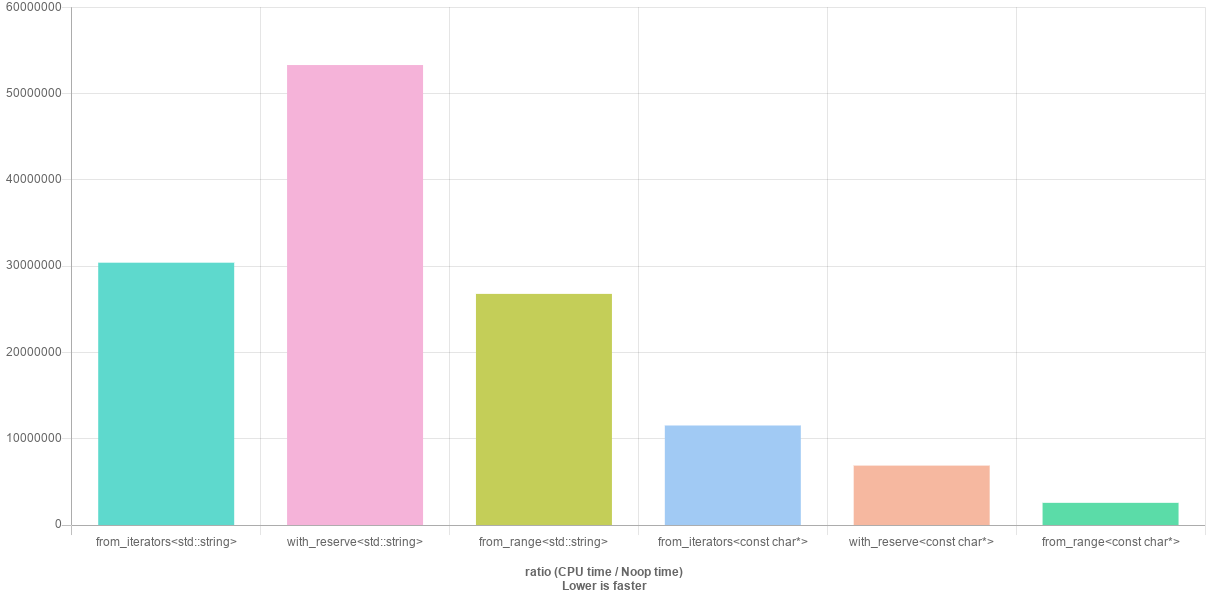
\includegraphics[width=\textwidth]{P1206_bench_a}
% https://quick-bench.com/q/aWpqVs5RODKoKJ0HPEBbslEn1Ds

In both scenarios, the \tcode{from_range} constructor performs significantly
better than both the iterator pair constructor and the reserve + copy method employed by \tcode{ranges::to}

Because \tcode{ranges::to} will call a tag constructor when there is one, it show the same difference.

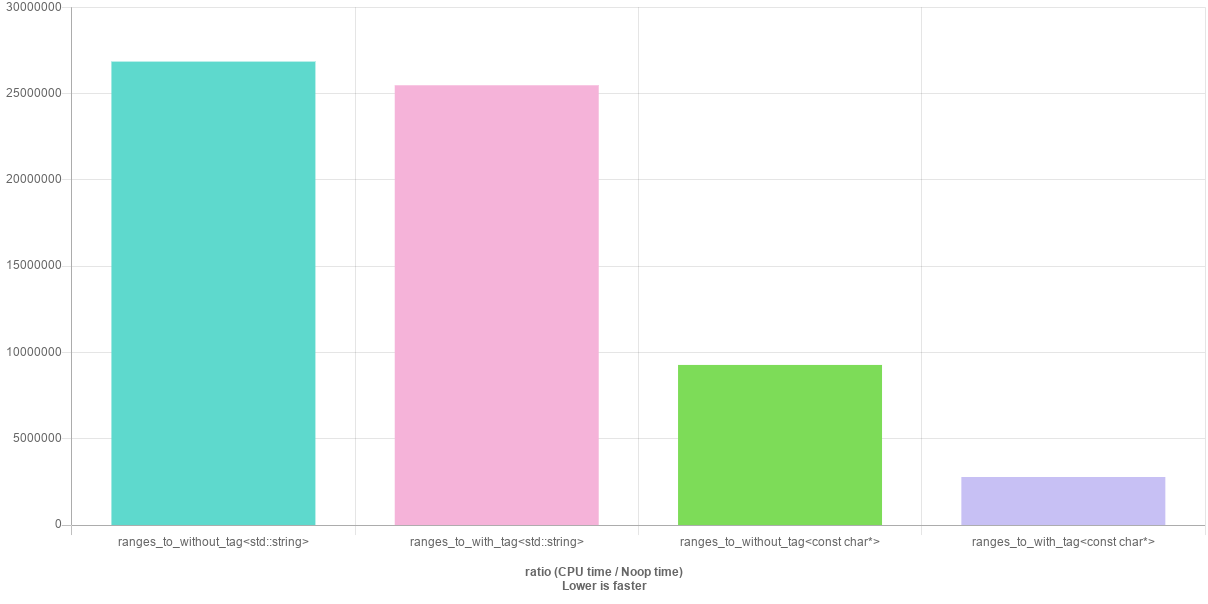
\includegraphics[width=\textwidth]{P1206_bench_b}

\href{https://quick-bench.com/q/sGkLaZF8I-d0-EOJETmAtVKKk9k}{{QuickBench}}



\subsection{Do we need iterator/sentinel pair constructors as well?}


The new standard library algorithms in the `std::ranges` namespace all provide multiple overloads taking both a range and an iterator/sentinel pair. This raises the question: should our new constructors provide a "range" overload (only), an iterator/sentinel pair overload (only), or both?

The second case (an iterator/sentinel pair only) is easily dismissed. There exist ranges which model \tcode{sized_range}, but whose iterators/sentinels do not model \tcode{sized_sentinel_for} - the canonical example being \tcode{std::list}. With such types, a constructor call like

\begin{colorblock}
std::list<int> list = get_list();
std::vector<int> vec(std::from_range, list); // copy into vector
\end{colorblock}

would know the size of the list and would therefore be able to allocate the required vector size upfront. On the other hand, a hypothetical call to

\begin{colorblock}
std::list<int> list = get_list();
std::vector<int> vec(std::from_range, list.begin(), list.end());
\end{colorblock}

cannot know the size of the input range upfront, and so would need two passes over the data.

We are thus left to decide whether to provide an iterator/sentinel constructor in addition to a "range" constructor. In the authors' opinion, this would be redundant. In cases where we do have separate iterator and sentinel objects that we wish to pass to a container constructor, we can do so using `subrange`, as in

\begin{colorblock}
std::vector vec(std::from_range, subrange(my_iter, my_sentinel));
\end{colorblock}

Furthermore, it is intended that users should be able to opt-in to \tcode{ranges::to} support for their own container classes by providing constructors which take \tcode{from_range_t} as their first argument. Adding iterator/sentinel constructors in addition to "range" constructors means more work for users to adhere to the protocol, and no doubt risks confusion about whether one, either, or both are required.

\subsection{\placeholder{reservable-container} concept}

The exposition only \placeholder{reservable-container} concepts checks for
\begin{itemize}
    \item \tcode{reserve}
    \item \tcode{max_size}
    \item \tcode{capacity}
\end{itemize}

which is consistent with ranges-v3. This serves multiple purposes:

\begin{itemize}
\item Avoid calling \tcode{reserve} on unordered containers and others entities that have a reserve method with different
semantics
\item Allow implementations to check that we are not trying to reserve more than max size
\end{itemize}


\section{Implementation Experience}

Implementations of \tcode{ranges::to} are available in \cite{Range V3}, \cite{cmcstl2} and on Github \cite{rangesnext}.
The tagged ranges constructors, insert methods and other range-taking container members fuctions have \textbf{not} been
implemented.

\section{Related Paper and future work}

Future work is needed to allow constructing \tcode{std::array} from \EXPO{tiny-ranges}.
This paper also do not proposes modifications of \tcode{path}(the author is not familiar with it enough) and \tcode{regex} (whose fate is in the balance).

\section{Previous polls}


\begin{quoteblock}
SG9 POLL: All range-based member functions should end with "_range" (e.g. assign_range, insert_range, append_range) except for the constructors which take tags.

\begin{tabular}{|c|c|c|c|c|}
\hline
F & N & A\\
\hline
7 & 1 & 0 \\
\hline
\end{tabular}
\end{quoteblock}

\begin{quoteblock}
SG9 POLL: We would like to add push_back_range, push_front_range to the relevant containers in the paper

\begin{tabular}{|c|c|c|c|c|}
    \hline
    F & N & A\\
    \hline
    6 & 3 & 0 \\
    \hline
\end{tabular}
\end{quoteblock}

\begin{quoteblock}
SG9 POLL: We approve the direction and design of D1206r4 with the recommended changes, and recommend forwarding it to LEWG

\begin{tabular}{|c|c|c|c|c|}
    \hline
    F & N & A\\
    \hline
    9 & 0 & 0 \\
    \hline
\end{tabular}
\end{quoteblock}


\section{Proposed wording}

Wording is relative to \cite{N4885}.


\rSec1[containers]{Containers}
\rSec1[container.requirements]{Container requirements}
\rSec2[container.requirements.general]{General container requirements}

\begin{itemize}
\item
\tcode{T} is
\defnx{\oldconcept{EmplaceConstructible} into \tcode{X} from \tcode{args}}
{\oldconceptname{EmplaceConstructible} into X from args@\oldconcept{EmplaceConstructible} into \tcode{X} from \tcode{args}},
for zero
or more arguments \tcode{args}, means that the following expression is well-formed:
\begin{codeblock}
    allocator_traits<A>::construct(m, p, args)
\end{codeblock}

\item
\tcode{T} is
\defnx{\oldconcept{Erasable} from \tcode{X}}
{\oldconceptname{Erasable} from X@\oldconcept{Erasable} from \tcode{X}}
means that the following expression is well-formed:
\begin{codeblock}
    allocator_traits<A>::destroy(m, p)
\end{codeblock}


\begin{note}
A container calls \tcode{allocator_traits<A>::construct(m, p, args)}
to construct an element at \tcode{p} using \tcode{args},
with \tcode{m == get_allocator()}.
The default \tcode{construct} in \tcode{allocator} will
call \tcode{::new((void*)p) T(args)},
but specialized allocators can choose a different definition.
\end{note}

\begin{addedblock}
    The following exposition-only concept is used in the definition of containers
\begin{codeblock}
template<class R, class T>
concept @\placeholdernc{range-compatible-with-container-range-construction}@ = // \expos
       ranges::input_range<R> &&
       convertible_to<range_reference_t<R>, T> &&
       constructible_from<T, ranges::range_reference_t<R>>;
\end{codeblock}
\end{addedblock}

\end{itemize}


\rSec2[sequence.reqmts]{Sequence containers}



In Tables [tab:container.seq.req]
and [tab:container.seq.opt],
\begin{itemize}
    \item
    \tcode{X} denotes a sequence container class,
    \item
    \tcode{a} denotes a value of type \tcode{X} containing elements of type \tcode{T},
    \item
    \tcode{u} denotes the name of a variable being declared,
    \item
    \tcode{A} denotes \tcode{X::allocator_type} if
    the \grammarterm{qualified-id} \tcode{X::allocator_type} is valid and denotes a
    type\iref{temp.deduct} and
    \tcode{allocator<T>} if it doesn't,
    \item
    \tcode{i} and \tcode{j}
    denote iterators that meet the \oldconcept{InputIterator} requirements
    and refer to elements implicitly convertible to \tcode{value_type},
    \item
    \tcode{[i, j)} denotes a valid range,
    \begin{addedblock}
        \item\tcode{range} denotes a value of type \tcode{R} such that
        \begin{itemize}
            \item \tcode{R} models \tcode{ranges::input_range},
            \item \tcode{is_constructible_v<T, ranges::range_reference_t<R>>} is \tcode{true}
        \end{itemize}
    \end{addedblock}
    \item
    \tcode{il} designates an object of type \tcode{initializer_list<value_type>},
    \item
    \tcode{n} denotes a value of type \tcode{X::size_type},
    \item
    \tcode{p} denotes a valid constant iterator to \tcode{a},
    \item
    \tcode{q} denotes a valid dereferenceable constant iterator to \tcode{a},
    \item
    \tcode{[q1, q2)} denotes a valid range of constant iterators in \tcode{a},
    \item
    \tcode{t} denotes an lvalue or a const rvalue of \tcode{X::value_type}, and
    \item
    \tcode{rv} denotes a non-const rvalue of \tcode{X::value_type}.
    \item
    \tcode{Args} denotes a template parameter pack;
    \item
    \tcode{args} denotes a function parameter pack with the pattern \tcode{Args\&\&}.
\end{itemize}

\pnum
The complexities of the expressions are sequence dependent.

\begin{libreqtab3}
    {Sequence container requirements (in addition to container)}
    {container.seq.req}
    \\ \topline
    \lhdr{Expression}       &   \chdr{Return type}  &   \rhdr{Assertion/note}       \\
    &                       &   \rhdr{pre-/post-condition}   \\ \capsep
    \endfirsthead
    \continuedcaption\\
    \hline
    \lhdr{Expression}       &   \chdr{Return type}  &   \rhdr{Assertion/note}       \\
    &                       &   \rhdr{pre-/post-condition}   \\ \capsep
    \endhead
    \tcode{X(n, t)}\br
    \tcode{X u(n, t);}   &
    &
    \expects \tcode{T} is
    \oldconcept{CopyInsertable} into \tcode{X}.\br
    \ensures \tcode{distance(begin(), end()) == n}\br
    \effects Constructs a sequence container with \tcode{n} copies of \tcode{t}  \\ \rowsep

    \tcode{X(i, j)}\br
    \tcode{X u(i, j);}   &
    &
    \expects \tcode{T} is \oldconcept{EmplaceConstructible} into \tcode{X} from \tcode{*i}.
    For \tcode{vector}, if the iterator does
    not meet the \oldconcept{\-Forward\-Iterator} requirements\iref{forward.iterators}, \tcode{T}
    is also
    \oldconcept{MoveInsertable} into \tcode{X}.\br
    \ensures \tcode{distance(begin(), end()) ==}
    \tcode{distance(i, j)}\br
    \effects Constructs a sequence container equal to the range \tcode{[i, j)}.
    Each iterator in the range \range{i}{j} is dereferenced exactly once. \\ \rowsep

    \tcode{\added{X(from_range, range)}}    &
    &
    \begin{addedblock}
    \expects \tcode{T} is \oldconcept{EmplaceConstructible} into \tcode{X} from \tcode{range_reference_t<R>}.
    For \tcode{vector}, if \tcode{R} models neither \libconcept{sized_range}\iref{range.sized}
    nor \libconcept{forward_range}\iref{range.refinements},
    \tcode{T} is also \oldconcept{MoveInsertable} into \tcode{X}.
    \effects Constructs a sequence container equal to the range \tcode{range}.
    Each iterator in the range \tcode{range} is dereferenced exactly once.

    \ensures \tcode{distance(begin(), end()) == ranges::distance(range)}\br
    \end{addedblock}  \\ \rowsep

    \tcode{X(il)}      &
    &
    Equivalent to \tcode{X(il.begin(), il.end())} \\ \rowsep

    \tcode{a = il}     &
    \tcode{X\&}               &
    \expects \tcode{T} is
    \oldconcept{CopyInsertable} into \tcode{X}
    and \oldconcept{CopyAssignable}.\br
    \effects Assigns the range \range{il.begin()}{il.end()} into \tcode{a}. All existing
    elements of \tcode{a} are either assigned to or destroyed.\br
    \returns\ \tcode{*this}.
    \\ \rowsep

    \tcode{a.emplace(p, args)}  &
    \tcode{iterator}            &
    \expects \tcode{T} is \oldconcept{EmplaceConstructible} into \tcode{X} from \tcode{args}. For \tcode{vector} and \tcode{deque},
    \tcode{T} is also
    \oldconcept{MoveInsertable} into \tcode{X} and \oldconcept{MoveAssignable}.\br
    \effects Inserts an object of type \tcode{T} constructed with
    \tcode{std::forward<\brk{}Args\brk{}>(\brk{}args)...} before \tcode{p}.
    \\ \rowsep

    \tcode{a.insert(p,t)}   &
    \tcode{iterator}       &
    \expects \tcode{T} is
    \oldconcept{CopyInsertable} into \tcode{X}. For \tcode{vector} and \tcode{deque},
    \tcode{T} is also \oldconcept{CopyAssignable}.\br
    \effects\ Inserts a copy of \tcode{t} before \tcode{p}. \\ \rowsep

    \tcode{a.insert(p,rv)}   &
    \tcode{iterator}       &
    \expects \tcode{T} is
    \oldconcept{MoveInsertable} into \tcode{X}. For \tcode{vector} and \tcode{deque},
    \tcode{T} is also \oldconcept{MoveAssignable}.\br
    \effects\ Inserts a copy of \tcode{rv} before \tcode{p}. \\ \rowsep

    \tcode{a.insert(p,n,t)}     &
    \tcode{iterator}               &
    \expects \tcode{T} is
    \oldconcept{CopyInsertable} into \tcode{X}
    and \oldconcept{CopyAssignable}.\br
    \effects Inserts \tcode{n} copies of \tcode{t} before \tcode{p}. \\ \rowsep

    \tcode{a.insert(p,i,j)}    &
    \tcode{iterator}           &
    \expects \tcode{T} is \oldconcept{EmplaceConstructible} into \tcode{X} from \tcode{*i}.
    For \tcode{vector} and \tcode{deque}, \tcode{T} is also
    \oldconcept{MoveInsertable} into \tcode{X}, \oldconcept{MoveConstructible}, \oldconcept{MoveAssignable},
    and swappable\iref{swappable.requirements}.
    Neither \tcode{i} nor \tcode{j} are iterators into \tcode{a}.\br
    \effects Inserts copies of elements in \tcode{[i, j)} before \tcode{p}.
    Each iterator in the range \range{i}{j} shall be dereferenced exactly once.  \\ \rowsep

    \tcode{\added{a.insert_range(p, range)}}    &
    \added{\tcode{iterator}} &
    \begin{addedblock}
        \expects For \tcode{vector} and \tcode{deque}, \tcode{range_reference_t<R>} is
        \oldconcept{MoveInsertable} into \tcode{X}, \oldconcept{MoveConstructible}, \oldconcept{MoveAssignable},
        and swappable\iref{swappable.requirements}.
        \tcode{range} and \tcode{*this} do not overlap.\br
        \effects Inserts copies of elements in \tcode{range} before \tcode{p}.
        Each iterator in the range \tcode{range} shall be dereferenced exactly once.
    \end{addedblock}  \\ \rowsep

    \tcode{X(il)}      &
    &
    Equivalent to \tcode{X(il.begin(), il.end())} \\ \rowsep

    \tcode{a.insert(p, il)}  &
    \tcode{iterator}            &
    \tcode{a.insert(p, il.begin(), il.end())}.  \\ \rowsep

    \tcode{a.erase(q)}  &
    \tcode{iterator}   &
    \expects For \tcode{vector} and \tcode{deque},
    \tcode{T} is \oldconcept{MoveAssignable}.\br
    \effects\ Erases the element pointed to by \tcode{q}. \\ \rowsep

    \tcode{a.erase(q1,q2)}  &
    \tcode{iterator}   &
    \expects For \tcode{vector} and \tcode{deque},
    \tcode{T} is \oldconcept{MoveAssignable}.\br
    \effects\ Erases the elements in the range \tcode{[q1, q2)}.  \\ \rowsep

    \tcode{a.clear()}   &
    \tcode{void}       &
    \effects Destroys all elements in \tcode{a}. Invalidates all references, pointers, and
    iterators referring to the elements of \tcode{a} and may invalidate the past-the-end iterator.\br
    \ensures \tcode{a.empty()} is \tcode{true}.\br
    \complexity Linear.      \\ \rowsep

    \tcode{a.assign(i,j)}   &
    \tcode{void}           &
    \expects \tcode{T} is \oldconcept{EmplaceConstructible} into \tcode{X} from \tcode{*i}
    and assignable from \tcode{*i}. For \tcode{vector}, if the iterator does not
    meet the forward iterator requirements\iref{forward.iterators}, \tcode{T}
    is also
    \oldconcept{MoveInsertable} into \tcode{X}.
    Neither \tcode{i} nor \tcode{j} are iterators into \tcode{a}.\br
    \effects
    Replaces elements in \tcode{a} with a copy of \tcode{[i, j)}.
    Invalidates all references, pointers and iterators
    referring to the elements of \tcode{a}.
    For \tcode{vector} and \tcode{deque},
    also invalidates the past-the-end iterator.
    Each iterator in the range \range{i}{j} shall be dereferenced exactly once.  \\ \rowsep

    \tcode{\added{a.assign_range(p, range)}}    &
    \added{\tcode{void}} &
    \begin{addedblock}
        \expects \tcode{range} and \tcode{*this} do not overlap.\br
         \effects
        Replaces elements in \tcode{a} with a copy of each element in \tcode{range}.
        Invalidates all references, pointers and iterators
        referring to the elements of \tcode{a}.
        For \tcode{vector} and \tcode{deque},
        also invalidates the past-the-end iterator.
        Each iterator in the range \tcode{range} shall be dereferenced exactly once.
    \end{addedblock}  \\ \rowsep



    \tcode{a.assign(il)}    &
    \tcode{void}          &
    \tcode{a.assign(il.begin(), il.end())}. \\ \rowsep

    \tcode{a.assign(n,t)}   &
    \tcode{void}           &
    \expects \tcode{T} is
    \oldconcept{CopyInsertable} into \tcode{X}
    and \oldconcept{CopyAssignable}.
    \tcode{t} is not a reference into \tcode{a}.\br
    \effects Replaces elements in \tcode{a} with \tcode{n} copies of \tcode{t}.
    Invalidates all references, pointers and iterators
    referring to the elements of \tcode{a}.
    For \tcode{vector} and \tcode{deque},
    also invalidates the past-the-end iterator.  \\
\end{libreqtab3}

\pnum
The iterator returned from
\tcode{a.insert(p, t)}
points to the copy of
\tcode{t}
inserted into
\tcode{a}.

\pnum
The iterator returned from \tcode{a.insert(p, rv)} points to the copy of \tcode{rv}
inserted into \tcode{a}.

\pnum
The iterator returned from \tcode{a.insert(p, n, t)} points to the copy of the first
element inserted into \tcode{a}, or \tcode{p} if \tcode{n == 0}.

\pnum
The iterator returned from \tcode{a.insert(p, i, j)} points to the copy of the first
element inserted into \tcode{a}, or \tcode{p} if \tcode{i == j}.

\begin{addedblock}
\pnum
The iterator returned from \tcode{a.insert_range(p, range)} points to the copy of the first
element inserted into \tcode{a}, or \tcode{p} if \tcode{ranges::empty(range)}.

\end{addedblock}

\pnum
The iterator returned from \tcode{a.insert(p, il)} points to the copy of the first
element inserted into \tcode{a}, or \tcode{p} if \tcode{il} is empty.

\pnum
The iterator returned from \tcode{a.emplace(p, args)} points to the new element
constructed from \tcode{args} into \tcode{a}.

\pnum
The iterator returned from
\tcode{a.erase(q)}
points to the element immediately following
\tcode{q}
prior to the element being erased.
If no such element exists,
\tcode{a.end()}
is returned.

\pnum
The iterator returned by
\tcode{a.erase(q1, q2)}
points to the element pointed to by
\tcode{q2}
prior to any elements being erased.
If no such element exists,
\tcode{a.end()}
is returned.

\pnum
For every sequence container defined in this Clause and in \ref{strings}:
\begin{itemize}
    \item If the constructor
    \begin{codeblock}
        template<class InputIterator>
        X(InputIterator first, InputIterator last,
        const allocator_type& alloc = allocator_type());
    \end{codeblock}
    is called with a type \tcode{InputIterator} that does not qualify as an input
    iterator, then the constructor
    shall not participate in overload resolution.

    \item If the member functions of the forms:
    \begin{codeblock}
        template<class InputIterator>
        @\placeholdernc{return-type}@ @\placeholdernc{F}@(const_iterator p,
        InputIterator first, InputIterator last);       // such as \tcode{insert}

        template<class InputIterator>
        @\placeholdernc{return-type}@ @\placeholdernc{F}@(InputIterator first, InputIterator last);       // such as \tcode{append}, \tcode{assign}

        template<class InputIterator>
        @\placeholdernc{return-type}@ @\placeholdernc{F}@(const_iterator i1, const_iterator i2,
        InputIterator first, InputIterator last);       // such as \tcode{replace}
    \end{codeblock}
    are called with a type \tcode{InputIterator} that does not qualify as an input
    iterator, then these functions
    shall not participate in overload resolution.

    \item A deduction guide for a sequence container shall not participate in overload resolution
    if it has an \tcode{InputIterator} template parameter and a type that does not
    qualify as an input iterator is deduced for that parameter,
    or if it has an \tcode{Allocator} template parameter and a type that does not
    qualify as an allocator is deduced for that parameter.
\end{itemize}

\pnum
\tref{container.seq.opt} lists operations
that are provided for some types of
sequence containers but not others.
An implementation shall provide
these operations for all container types shown in the ``container''
column, and shall implement them so as to take amortized constant
time.

\begin{libreqtab4a}
    {Optional sequence container operations}
    {container.seq.opt}
    \\ \topline
    \lhdr{Expression}       &   \chdr{Return type}  &   \chdr{Operational semantics}       &   \rhdr{Container}    \\ \capsep
    \endfirsthead
    \continuedcaption\\
    \hline
    \lhdr{Expression}       &   \chdr{Return type}  &   \chdr{Operational semantics}       &   \rhdr{Container}    \\ \capsep
    \endhead

    \tcode{a.front()}       &
    \tcode{reference; const_reference} for constant \tcode{a}    &
    \tcode{*a.begin()}     &
    \tcode{basic_string},
    \tcode{array},
    \tcode{deque},
    \tcode{forward_list},
    \tcode{list},
    \tcode{vector}
    \\ \rowsep

    \tcode{a.back()}        &
    \tcode{reference; const_reference} for constant \tcode{a}    &
    \tcode{\{ auto tmp = a.end();}\br
    \tcode{    --tmp;}\br
    \tcode{    return *tmp; \}}    &
    \tcode{basic_string},
    \tcode{array},
    \tcode{deque},
    \tcode{list},
    \tcode{vector}
    \\ \rowsep

    \tcode{a.emplace_\-front(args)}      &
    \tcode{reference}                &
    \effects Prepends an object of type \tcode{T} constructed with \tcode{std::forward<\brk{}Args\brk{}>(\brk{}args)...}.\br
    \expects \tcode{T} is \oldconcept{EmplaceConstructible} into \tcode{X} from \tcode{args}.\br
    \returns \tcode{a.front()}.  &
    \tcode{deque},
    \tcode{forward_list},
    \tcode{list}
    \\ \rowsep

    \tcode{a.emplace_\-back(args)}      &
    \tcode{reference}                &
    \effects Appends an object of type \tcode{T} constructed with \tcode{std::forward<\brk{}Args\brk{}>(\brk{}args)...}.\br
    \expects \tcode{T} is \oldconcept{EmplaceConstructible} into \tcode{X} from \tcode{args}. For \tcode{vector}, \tcode{T}
    is also
    \oldconcept{MoveInsertable} into \tcode{X}.
    \returns \tcode{a.back()}.  &
    \tcode{deque},
    \tcode{list},
    \tcode{vector}
    \\ \rowsep

    \tcode{a.push_front(t)} &
    \keyword{void}          &
    \effects Prepends a copy of \tcode{t}.\br
    \expects \tcode{T} is
    \oldconcept{CopyInsertable} into \tcode{X}.
    &
    \tcode{deque},
    \tcode{forward_list},
    \tcode{list}
    \\ \rowsep


    \tcode{a.push_front(rv)} &
    \keyword{void}          &
    \effects Prepends a copy of \tcode{rv}.\br
    \expects \tcode{T} is
    \oldconcept{MoveInsertable} into \tcode{X}.
    &
    \tcode{deque},
    \tcode{forward_list},
    \tcode{list}
    \\ \rowsep


    \begin{addedblock}\tcode{a.prepend_range(range)}\end{addedblock} &
    \added{\keyword{void}}          &
    \begin{addedblock}
        \effects \effects Inserts copies of elements in \tcode{range} before \tcode{begin()}.
        Each iterator in the range \tcode{range} shall be dereferenced exactly once. The order of elements in \tcode{range}
        is not reversed.
        \expects \tcode{T} is
        \oldconcept{CopyInsertable} into \tcode{X}.
    \end{addedblock}
    &
    \added{
        \tcode{deque},
        \tcode{forward_list},
        \tcode{list}}
    \\ \rowsep


    \tcode{a.push_back(t)} &
    \keyword{void}          &
    \effects Appends a copy of \tcode{t}.\br
    \expects \tcode{T} is
    \oldconcept{CopyInsertable} into \tcode{X}.
    &
    \tcode{basic_string},
    \tcode{deque},
    \tcode{list},
    \tcode{vector}
    \\ \rowsep

    \tcode{a.push_back(rv)} &
    \keyword{void}          &
    \effects Appends a copy of \tcode{rv}.\br
    \expects \tcode{T} is
    \oldconcept{MoveInsertable} into \tcode{X}.
    &
    \tcode{basic_string},
    \tcode{deque},
    \tcode{list},
    \tcode{vector}
    \\ \rowsep


    \begin{addedblock}\tcode{a.append_range(range)}\end{addedblock} &
    \added{\keyword{void}}          &
    \begin{addedblock}
        \effects \effects Inserts copies of elements in \tcode{range} before \tcode{end()}.
        Each iterator in the range \tcode{range} shall be dereferenced exactly once.
        \expects \tcode{T} is
        \oldconcept{CopyInsertable} into \tcode{X}.
    \end{addedblock}
    &
    \added{
        \tcode{basic\char`_string},
        \tcode{deque},
        \tcode{list},
        \tcode{vector}}
    \\ \rowsep

    \tcode{a.pop_front()}      &
    \keyword{void}               &
    \effects Destroys the first element.\br
    \expects \tcode{a.empty()} is \tcode{false}. &
    \tcode{deque},
    \tcode{forward_list},
    \tcode{list}
    \\ \rowsep

    \tcode{a.pop_back()}       &
    \keyword{void}               &
    \effects Destroys the last element.\br
    \expects \tcode{a.empty()} is \tcode{false}. &
    \tcode{basic_string},
    \tcode{deque},
    \tcode{list},
    \tcode{vector}
    \\ \rowsep

    \tcode{a[n]}                &
    \tcode{reference; const_reference} for constant \tcode{a}    &
    \tcode{*(a.begin() + n)}   &
    \tcode{basic_string},
    \tcode{array},
    \tcode{deque},
    \tcode{vector}
    \\ \rowsep

    \tcode{a.at(n)}             &
    \tcode{reference; const_reference} for constant \tcode{a}    &
    \tcode{*(a.begin() + n)}   &
    \tcode{basic_string},
    \tcode{array},
    \tcode{deque},
    \tcode{vector}
    \\

\end{libreqtab4a}

\pnum
The member function
\tcode{at()}
provides bounds-checked access to container elements.
\tcode{at()}
throws
\tcode{out_of_range}
if
\tcode{n >= a.size()}.



\rSec2[associative.reqmts]{Associative containers}

\rSec3[associative.reqmts.general]{General}

\pnum
Associative containers provide fast retrieval of data based on keys.
The library provides four basic kinds of associative containers:
\tcode{set},
\tcode{multiset},
\tcode{map}
and
\tcode{multimap}.

\pnum
Each associative container is parameterized on
\tcode{Key}
and an ordering relation
\tcode{Compare}
that induces a strict weak ordering\iref{alg.sorting} on
elements of
\tcode{Key}.
In addition,
\tcode{map}
and
\tcode{multimap}
associate an arbitrary \term{mapped type}
\tcode{T}
with the
\tcode{Key}.
The object of type
\tcode{Compare}
is called the
\term{comparison object}
of a container.

\pnum
The phrase ``equivalence of keys'' means the equivalence relation imposed by the
comparison object.
That is, two keys
\tcode{k1}
and
\tcode{k2}
are considered to be equivalent if for the
comparison object
\tcode{comp},
\tcode{comp(k1, k2) == false \&\& comp(k2, k1) == false}.
\begin{note}
    This is not necessarily the same as the result of \tcode{k1 == k2}.
\end{note}
For any two keys
\tcode{k1}
and
\tcode{k2}
in the same container, calling
\tcode{comp(k1, k2)}
shall always return the same value.

\pnum
An associative container supports \term{unique keys} if it may contain at
most one element for each key. Otherwise, it supports \term{equivalent keys}.
The \tcode{set} and \tcode{map} classes support unique keys; the \tcode{multiset}
and \tcode{multimap} classes support equivalent keys.
For \tcode{multiset} and \tcode{multimap},
\tcode{insert}, \tcode{emplace}, and \tcode{erase} preserve the relative ordering
of equivalent elements.

\pnum
For \tcode{set} and \tcode{multiset} the value type is the same as the key type.
For \tcode{map} and \tcode{multimap} it is equal to \tcode{pair<const Key, T>}.

\pnum
\tcode{iterator}
of an associative container is of the bidirectional iterator category.
For associative containers where the value type is the same as the key type, both
\tcode{iterator}
and
\tcode{const_iterator}
are constant iterators. It is unspecified whether or not
\tcode{iterator}
and
\tcode{const_iterator}
are the same type.
\begin{note}
    \tcode{iterator} and \tcode{const_iterator} have identical semantics in this case, and \tcode{iterator} is convertible to \tcode{const_iterator}. Users can avoid violating the one-definition rule by always using \tcode{const_iterator} in their function parameter lists.
\end{note}

\pnum
The associative containers meet all the requirements of Allocator-aware
containers\iref{container.requirements.general}, except that for
\tcode{map} and \tcode{multimap}, the requirements placed on \tcode{value_type}
in \tref{container.alloc.req} apply instead to \tcode{key_type}
and \tcode{mapped_type}.
\begin{note}
    For example, in some cases \tcode{key_type} and \tcode{mapped_type}
    are required to be \oldconcept{CopyAssignable} even though the associated
    \tcode{value_type}, \tcode{pair<const key_type, mapped_type>}, is not
    \oldconcept{CopyAssignable}.
\end{note}

\pnum
In \tref{container.assoc.req},
\begin{itemize}
    \item
    \tcode{X} denotes an associative container class,
    \item
    \tcode{a} denotes a value of type \tcode{X},
    \item
    \tcode{a2} denotes a value of a type with nodes compatible with type
    \tcode{X} (\tref{container.node.compat}),
    \item
    \tcode{b} denotes a possibly \tcode{const} value of type \tcode{X},
    \item
    \tcode{u} denotes the name of a variable being declared,
    \item
    \tcode{a_uniq} denotes a value of type \tcode{X}
    when \tcode{X} supports unique keys,
    \item
    \tcode{a_eq} denotes a value of type \tcode{X}
    when \tcode{X} supports multiple keys,
    \item
    \tcode{a_tran} denotes a possibly \tcode{const} value of type \tcode{X}
    when the \grammarterm{qualified-id}
    \tcode{X::key_compare::is_transpa\-rent} is valid
    and denotes a type\iref{temp.deduct},
    \item
    \tcode{i} and \tcode{j}
    meet the \oldconcept{InputIterator} requirements and refer to elements
    implicitly convertible to
    \tcode{value_type},
    \item
    \range{i}{j} denotes a valid range,
    \begin{addedblock}
        \item\tcode{range} denotes a value of type \tcode{R} such that
        \begin{itemize}
            \item \tcode{R} models \tcode{ranges::input_range}.
            \item \tcode{is_constructible<typename X::value_type, ranges::range_reference_t<R>>} is \tcode{true}.
        \end{itemize}
    \end{addedblock}
    \item
    \tcode{p} denotes a valid constant iterator to \tcode{a},
    \item
    \tcode{q} denotes a valid dereferenceable constant iterator to \tcode{a},
    \item
    \tcode{r} denotes a valid dereferenceable iterator to \tcode{a},
    \item
    \tcode{[q1, q2)} denotes a valid range of constant iterators in \tcode{a},
    \item
    \tcode{il} designates an object of type \tcode{initializer_list<value_type>},
    \item
    \tcode{t} denotes a value of type \tcode{X::value_type},
    \item
    \tcode{k} denotes a value of type \tcode{X::key_type}, and
    \item
    \tcode{c} denotes a possibly \tcode{const} value of type \tcode{X::key_compare};
    \item
    \tcode{kl} is a value such that \tcode{a} is partitioned\iref{alg.sorting}
    with respect to \tcode{c(r, kl)}, with \tcode{r} the key value of \tcode{e}
    and \tcode{e} in \tcode{a};
    \item
    \tcode{ku} is a value such that \tcode{a} is partitioned with respect to
    \tcode{!c(ku, r)};
    \item
    \tcode{ke} is a value such that \tcode{a} is partitioned with respect to
    \tcode{c(r, ke)} and \tcode{!c(ke, r)}, with \tcode{c(r, ke)} implying
    \tcode{!c(ke, r)}.
    \item
    \tcode{A} denotes the storage allocator used by \tcode{X}, if any, or \tcode{allocator<X::value_type>} otherwise,
    \item
    \tcode{m} denotes an allocator of a type convertible to \tcode{A},
    and \tcode{nh} denotes a non-const rvalue of type \tcode{X::node_type}.
\end{itemize}

% Local command to index names as members of all ordered containers.
\newcommand{\indexordmem}[1]{%
    \indexlibrary{\idxcode{#1}!ordered associative containers}%
    \indexlibrary{\idxcode{set}!\idxcode{#1}}%
    \indexlibrary{\idxcode{map}!\idxcode{#1}}%
    \indexlibrary{\idxcode{multiset}!\idxcode{#1}}%
    \indexlibrary{\idxcode{multimap}!\idxcode{#1}}%
}

\begin{libreqtab4b}
    {Associative container requirements (in addition to container)}
    {container.assoc.req}
    \\ \topline
    \lhdr{Expression}       &   \chdr{Return type}  &   \chdr{Assertion/note}       &   \rhdr{Complexity}   \\
    &                       &   \chdr{pre-/post-condition}   &                       \\ \capsep
    \endfirsthead
    \continuedcaption\\
    \hline
    \lhdr{Expression}       &   \chdr{Return type}  &   \chdr{Assertion/note}       &   \rhdr{Complexity}   \\
    &                       &   \chdr{pre-/post-condition}   &                       \\ \capsep
    \endhead

    \tcode{X(i,j,c)}\br
    \tcode{X~u(i,j,c);}     &
    &
    \expects \tcode{value_type} is \oldconcept{EmplaceConstructible} into \tcode{X} from \tcode{*i}.\br
    \effects\ Constructs an empty container and inserts elements from the
    range \tcode{[i, j)} into it; uses \tcode{c} as a comparison object. &
    $N \log N$ in general, where $N$ has the value \tcode{distance(i, j)};
    linear if \tcode{[i, j)} is sorted with \tcode{value_comp()} \\ \rowsep

    \tcode{X(i,j)}\br\tcode{X~u(i,j);}    &
    &
    \expects \tcode{key_compare} meets the \oldconcept{DefaultConstructible} requirements.
    \tcode{value_type} is \oldconcept{EmplaceConstructible} into \tcode{X} from \tcode{*i}.\br
    \effects\ Same as above, but uses \tcode{Compare()} as a comparison object.  &
    same as above                      \\ \rowsep


    \tcode{\added{X(from_range, range, c)}}    &
    &
    \begin{addedblock}
        \effects Constructs an empty container and insert each element from \tcode{range} into it.
        Uses C as the comparison object.
    \end{addedblock}  &
    \begin{addedblock}
        $N \log N$ in general, where $N$ has the value \tcode{ranges::distance(range)};
        linear if \tcode{range} is sorted with \tcode{value_comp()}
    \end{addedblock}

         \\ \rowsep

    \tcode{\added{X(from_range, range)}}    &
    &
    \begin{addedblock}
        \expects \tcode{key_compare} meets the \oldconcept{DefaultConstructible} requirements.
        \effects Constructs an empty container and insert each element from \tcode{range} into it.
        Uses Compare() as the comparison object.
    \end{addedblock}
     &
     \begin{addedblock}
     same as above
     \end{addedblock}
      \\ \rowsep

    \tcode{X(il)}            &
    &
    same as \tcode{X(il.begin(), il.end())}  &
    same as \tcode{X(il.begin(), il.end())}  \\ \rowsep

    \tcode{X(il,c)}          &
    &
    same as \tcode{X(il.begin(), il.end(), c)}  &
    same as \tcode{X(il.begin(), il.end(), c)}  \\ \rowsep

    \tcode{a = il}     &
    \tcode{X\&}               &
    \expects \tcode{value_type} is
    \oldconcept{CopyInsertable} into \tcode{X}
    and \oldconcept{CopyAssignable}.\br
    \effects Assigns the range \range{il.begin()}{il.end()} into \tcode{a}. All
    existing elements of \tcode{a} are either assigned to or destroyed. &
    $N \log N$ in general, where $N$ has the value \tcode{il.size() + a.size()};
    linear if \range{il.begin()}{il.end()} is sorted with \tcode{value_comp()}
    \\ \rowsep

    \tcode{a.\brk{}insert(\brk{}i, j)}          &
    \tcode{void}                   &
    \expects \tcode{value_type} is \oldconcept{EmplaceConstructible} into \tcode{X} from \tcode{*i}.
    Neither \tcode{i} nor \tcode{j} are iterators into \tcode{a}.\br
    \effects Inserts each element from the range \range{i}{j} if and only if there
    is no element with key equivalent to the key of that element in containers
    with unique keys; always inserts that element in containers with equivalent keys.  &
    $N \log (\tcode{a.size()} + N)$, where $N$ has the value \tcode{distance(i, j)} \\ \rowsep


   \added{\tcode{a.insert\char`_range(range)}}         &
   \linebreak \tcode{void}                   &
   \begin{addedblock}
   \expects \tcode{value_type} is \oldconcept{EmplaceConstructible} into \tcode{X} from \tcode{range_reference_t<R>}.
   Neither \tcode{range} and \tcode{a} do not overlap.\br
   \effects Inserts each element from \tcode{range} if and only if there
   is no element with key equivalent to the key of that element in containers
   with unique keys; always inserts that element in containers with equivalent keys.
   \end{addedblock}  &
   \begin{addedblock}
   $N \log (\tcode{a.size()} + N)$, where $N$ has the value \tcode{ranges::distance(range)}
   \end{addedblock} \\ \rowsep


\end{libreqtab4b}

\pnum
The \tcode{insert}\added{, \tcode{insert\char`_range}} and \tcode{emplace} members shall not affect the validity of
iterators and references to the container,
and the \tcode{erase} members shall invalidate only iterators and
references to the erased elements.

\pnum
The \tcode{extract} members invalidate only iterators to the removed element;
pointers and references to the removed element remain valid. However, accessing
the element through such pointers and references while the element is owned by
a \tcode{node_type} is undefined behavior. References and pointers to an element
obtained while it is owned by a \tcode{node_type} are invalidated if the element
is successfully inserted.

\pnum
The fundamental property of iterators of associative containers is that they iterate through the containers
in the non-descending order of keys where non-descending is defined by the comparison that was used to
construct them.
For any two dereferenceable iterators
\tcode{i}
and
\tcode{j}
such that distance from
\tcode{i}
to
\tcode{j}
is positive, the following condition holds:

\begin{codeblock}
    value_comp(*j, *i) == false
\end{codeblock}

\pnum
For associative containers with unique keys the stronger condition holds:

\begin{codeblock}
    value_comp(*i, *j) != false
\end{codeblock}

\pnum
When an associative container is constructed by passing a comparison object the
container shall not store a pointer or reference to the passed object,
even if that object is passed by reference.
When an associative container is copied, through either a copy constructor
or an assignment operator,
the target container shall then use the comparison object from the container
being copied,
as if that comparison object had been passed to the target container in
its constructor.

\pnum
The member function templates
\tcode{find}, \tcode{count}, \tcode{contains},
\tcode{lower_bound}, \tcode{upper_bound}, and \tcode{equal_range}
shall not participate in overload resolution unless
the \grammarterm{qualified-id} \tcode{Compare::is_transparent} is valid
and denotes a type\iref{temp.deduct}.

\pnum
A deduction guide for an associative container shall not participate in overload resolution
if any of the following are true:
\begin{itemize}
    \item It has an \tcode{InputIterator} template parameter
    and a type that does not qualify as an input iterator is deduced for that parameter.

    \item It has an \tcode{Allocator} template parameter
    and a type that does not qualify as an allocator is deduced for that parameter.

    \item It has a \tcode{Compare} template parameter
    and a type that qualifies as an allocator is deduced for that parameter.
\end{itemize}


\rSec3[unord.req.general]{General}

// ...

\pnum
\indextext{unordered associative containers}%
\indextext{unordered associative containers!requirements}%
\indextext{requirements!unordered associative container}%
\indextext{unordered associative containers!unique keys}%
\indextext{unordered associative containers!equivalent keys}%
\indextext{requirements!container}%
In \tref{container.hash.req},
\begin{itemize}
    \item
    \tcode{X} denotes an unordered associative container class,
    \item
    \tcode{a} denotes a value of type \tcode{X},
    \item
    \tcode{a2} denotes a value of a type with nodes compatible
    with type \tcode{X} (\tref{container.node.compat}),
    \item
    \tcode{b} denotes a possibly const value of type \tcode{X},
    \item
    \tcode{a_uniq} denotes a value of type \tcode{X}
    when \tcode{X} supports unique keys,
    \item
    \tcode{a_eq} denotes a value of type \tcode{X}
    when \tcode{X} supports equivalent keys,
    \item
    \tcode{a_tran} denotes a possibly const value of type \tcode{X}
    when the \grammarterm{qualified-id}s
    \tcode{X::key_equal::is_transparent} and
    \tcode{X::hasher::is_transparent}
    are both valid and denote types\iref{temp.deduct},
    \item
    \tcode{i} and \tcode{j} denote input iterators
    that refer to \tcode{value_type},
    \item
    \tcode{[i, j)} denotes a valid range,
    \begin{addedblock}
    \item\tcode{range} denotes a value of type \tcode{R} such that
    \begin{itemize}
        \item \tcode{R} models \tcode{ranges::input_range}.
        \item \tcode{is_constructible<value_type, ranges::range_reference_t<R>>} is \tcode{true}.
    \end{itemize}
    \end{addedblock}
    \item
    \tcode{p} and \tcode{q2} denote valid constant iterators to \tcode{a},
    \item
    \tcode{q} and \tcode{q1} denote
    valid dereferenceable constant iterators to \tcode{a},
    \item
    \tcode{r} denotes a valid dereferenceable iterator to \tcode{a},
    \item
    \tcode{[q1, q2)} denotes a valid range in \tcode{a},
    \item
    \tcode{il} denotes a value of type \tcode{initializer_list<value_type>},
    \item
    \tcode{t} denotes a value of type \tcode{X::value_type},
    \item
    \tcode{k} denotes a value of type \tcode{key_type},
    \item
    \tcode{hf} denotes a possibly const value of type \tcode{hasher},
    \item
    \tcode{eq} denotes a possibly const value of type \tcode{key_equal},
    \item
    \tcode{ke} is a value such that
    \begin{itemize}
        \item \tcode{eq(r1, ke) == eq(ke, r1)}
        \item \tcode{hf(r1) == hf(ke)} if \tcode{eq(r1, ke)} is \tcode{true}, and
        \item \tcode{(eq(r1, ke) \&\& eq(r1, r2)) == eq(r2, ke)}
    \end{itemize}
    where \tcode{r1} and \tcode{r2} are keys of elements in \tcode{a_tran},
    \item
    \tcode{n} denotes a value of type \tcode{size_type},
    \item
    \tcode{z} denotes a value of type \tcode{float}, and
    \item
    \tcode{nh} denotes a non-const rvalue of type \tcode{X::node_type}.
\end{itemize}

% Local command to index names as members of all unordered containers.
\newcommand{\indexunordmem}[1]{%
    \indexlibrary{\idxcode{#1}!unordered associative containers}%
    \indexlibrary{\idxcode{unordered_set}!\idxcode{#1}}%
    \indexlibrary{\idxcode{unordered_map}!\idxcode{#1}}%
    \indexlibrary{\idxcode{unordered_multiset}!\idxcode{#1}}%
    \indexlibrary{\idxcode{unordered_multimap}!\idxcode{#1}}%
}

\begin{libreqtab4d}
    {Unordered associative container requirements (in addition to container)}
    {container.hash.req}
    \\ \topline
    \lhdr{Expression} & \chdr{Return type}   & \chdr{Assertion/note}      & \rhdr{Complexity} \\
    &                      & \chdr{pre-/post-condition} & \\ \capsep
    \endfirsthead
    \continuedcaption\\
    \hline
    \lhdr{Expression} & \chdr{Return type}   & \chdr{Assertion/note}      & \rhdr{Complexity} \\
    &                      & \chdr{pre-/post-condition} & \\ \capsep
    \endhead
    %%

    \tcode{X(i, j, n, hf, eq)}\br \tcode{X a(i, j, n, hf, eq);}
    &   \tcode{X}
    &   \expects \tcode{value_type} is \oldconcept{EmplaceConstructible} into \tcode{X} from \tcode{*i}.\br
    \effects\ Constructs an empty container with at least \tcode{n} buckets,
    using \tcode{hf} as the hash function and \tcode{eq} as the key
    equality predicate, and inserts elements from \tcode{[i, j)} into it.
    &   Average case \bigoh{N} ($N$ is \tcode{distance(i, j)}), worst case
    \bigoh{N^2}
    \\ \rowsep
    %
    \tcode{X(i, j, n, hf)}\br \tcode{X a(i, j, n, hf);}
    &   \tcode{X}
    &   \expects \tcode{key_equal} meets the \oldconcept{DefaultConstructible} requirements.
    \tcode{value_type} is \oldconcept{EmplaceConstructible} into \tcode{X} from \tcode{*i}.\br
    \effects\ Constructs an empty container with at least \tcode{n} buckets,
    using \tcode{hf} as the hash function and \tcode{key_equal()} as the key
    equality predicate, and inserts elements from \tcode{[i, j)} into it.
    &   Average case \bigoh{N} ($N$ is \tcode{distance(i, j)}), worst case
    \bigoh{N^2}
    \\ \rowsep
    %
    \tcode{X(i, j, n)}\br \tcode{X a(i, j, n);}
    &   \tcode{X}
    &   \expects \tcode{hasher} and \tcode{key_equal} meet the \oldconcept{DefaultConstructible} requirements.
    \tcode{value_type} is \oldconcept{EmplaceConstructible} into \tcode{X} from \tcode{*i}.\br
    \effects\ Constructs an empty container with at least \tcode{n} buckets,
    using \tcode{hasher()} as the hash function and \tcode{key_equal()}
    as the key equality predicate, and inserts elements from \tcode{[i, j)}
    into it.
    &   Average case \bigoh{N} ($N$ is \tcode{distance(i, j)}), worst case
    \bigoh{N^2}
    \\ \rowsep
    %
    \tcode{X(i, j)}\br \tcode{X a(i, j);}
    &   \tcode{X}
    &   \expects \tcode{hasher} and \tcode{key_equal} meet the \oldconcept{DefaultConstructible} requirements.
    \tcode{value_type} is \oldconcept{EmplaceConstructible} into \tcode{X} from \tcode{*i}.\br
    \effects\ Constructs an empty container with an unspecified number of
    buckets, using \tcode{hasher()} as the hash function and
    \tcode{key_equal()} as the key equality predicate, and inserts elements
    from \tcode{[i, j)} into it.
    &   Average case \bigoh{N} ($N$ is \tcode{distance(i, j)}), worst case
    \bigoh{N^2}
    \\ \rowsep


    %% -----

    \begin{addedblock}
    \tcode{X(from_range, range, n, hf, eq)}\br \tcode{X a(from_range, range, n, hf, eq);}
    \end{addedblock}
    &
    \begin{addedblock}
    \tcode{X}
    \end{addedblock}
    &
    \begin{addedblock}
    \expects \tcode{value_type} is \oldconcept{EmplaceConstructible} into \tcode{X} from \tcode{range_reference_t<R>}.\br
    \effects\ Constructs an empty container with at least \tcode{n} buckets,
    using \tcode{hf} as the hash function and \tcode{eq} as the key
    equality predicate, and inserts each element from \tcode{range} into it.
    \end{addedblock}
    &
    \begin{addedblock}
    Average case \bigoh{N} ($N$ is \tcode{ranges::distance(range)}), worst case
    \bigoh{N^2}
    \end{addedblock}
    \\ \rowsep
    %
    \begin{addedblock}
    \tcode{X(from_range, range, n, hf)}\br \tcode{X a(from_range, range, n, hf);}
    \end{addedblock}
    &
    \begin{addedblock}
        \tcode{X}
    \end{addedblock}
    &
    \begin{addedblock}
    \expects \tcode{key_equal} meets the \oldconcept{DefaultConstructible} requirements.
    \tcode{value_type} is \oldconcept{EmplaceConstructible} into \tcode{X} from \tcode{range_reference_t<R>}.\br
    \effects\ Constructs an empty container with at least \tcode{n} buckets,
    using \tcode{hf} as the hash function and \tcode{key_equal()} as the key
    equality predicate, and inserts elements from \tcode{range} into it.
    \end{addedblock}
    &
    \begin{addedblock}
    Average case \bigoh{N} ($N$ is \tcode{distance(range)}), worst case
    \bigoh{N^2}
    \end{addedblock}
    \\ \rowsep
    %
    \begin{addedblock}
    \tcode{X(from_range, range, n)}\br \tcode{X a(from_range, range, n);} \end{addedblock}
    &
    \begin{addedblock} \tcode{X} \end{addedblock}
    &
    \begin{addedblock}
    \expects \tcode{hasher} and \tcode{key_equal} meet the \oldconcept{DefaultConstructible} requirements.
    \tcode{value_type} is \oldconcept{EmplaceConstructible} into \tcode{X} from  \tcode{range_reference_t<R>}.\br
    \effects\ Constructs an empty container with at least \tcode{n} buckets,
    using \tcode{hasher()} as the hash function and \tcode{key_equal()}
    as the key equality predicate, and inserts elements from \tcode{range}
    into it.
    \end{addedblock}
    &
    \begin{addedblock}
    Average case \bigoh{N} ($N$ is \tcode{ranges::distance(range)}), worst case
    \bigoh{N^2}
    \end{addedblock}
    \\ \rowsep
    %
    \begin{addedblock}
    \tcode{X(from_range, range)}\br \tcode{X a(from_range, range);}
    \end{addedblock}
    &

    \begin{addedblock} \tcode{X} \end{addedblock}
    &
    \begin{addedblock}
    \expects \tcode{hasher} and \tcode{key_equal} meet the \oldconcept{DefaultConstructible} requirements.
    \tcode{value_type} is \oldconcept{EmplaceConstructible} into \tcode{X} from  \tcode{range_reference_t<R>}.\br
    \effects\ Constructs an empty container with an unspecified number of
    buckets, using \tcode{hasher()} as the hash function and
    \tcode{key_equal()} as the key equality predicate, and inserts elements
    from \tcode{range} into it.
    \end{addedblock}
    &
    \begin{addedblock}
    Average case \bigoh{N} ($N$ is \tcode{ranges::distance(range)}), worst case
    \bigoh{N^2}
    \end{addedblock}
    \\ \rowsep

    %% -----






    %
    \tcode{X(il)}
    &   \tcode{X}
    &   Same as \tcode{X(il.begin(), il.end())}.
    &   Same as \tcode{X(il.begin(),} \tcode{il.end())}.
    \\ \rowsep
    %

    \indexunordmem{insert}%
    \tcode{a_uniq.insert(t)}
    &   \tcode{pair<iterator, bool>}
    &   \expects If \tcode{t} is a non-const rvalue, \tcode{value_type} is
    \oldconcept{MoveInsertable} into \tcode{X}; otherwise, \tcode{value_type} is
    \oldconcept{CopyInsertable} into \tcode{X}.\br
    \effects\ Inserts \tcode{t} if and only if there is no element in the container
    with key equivalent to the key of \tcode{t}.  The \tcode{bool}
    component of the returned pair indicates whether the insertion
    takes place, and the \tcode{iterator} component points to the element
    with key equivalent to the key of \tcode{t}.%
    &   Average case \bigoh{1}, worst case \bigoh{\tcode{a_uniq.}\br\tcode{size()}}.
    \\ \rowsep
    %
    \tcode{a_eq.insert(t)}
    &   \tcode{iterator}
    &   \expects If \tcode{t} is a non-const rvalue, \tcode{value_type} is
    \oldconcept{MoveInsertable} into \tcode{X}; otherwise, \tcode{value_type} is
    \oldconcept{CopyInsertable} into \tcode{X}.\br
    \effects\ Inserts \tcode{t}, and returns an iterator pointing to the newly
    inserted element.
    &   Average case \bigoh{1}, worst case \bigoh{\tcode{a_eq.}\br\tcode{size()}}.
    \\ \rowsep
    %
    \tcode{a.insert(p, t)}
    &   \tcode{iterator}
    &   \expects If \tcode{t} is a non-const rvalue, \tcode{value_type} is
    \oldconcept{MoveInsertable} into \tcode{X}; otherwise, \tcode{value_type} is
    \oldconcept{CopyInsertable} into \tcode{X}.\br
    \effects Equivalent to \tcode{a.insert(t)}.  Return value is an iterator pointing
    to the element with the key equivalent to that of \tcode{t}.  The
    iterator \tcode{p} is a hint pointing to where the search should
    start.  Implementations are permitted to ignore the hint.%
    &   Average case \bigoh{1}, worst case \bigoh{\tcode{a.size()}}.
    \\ \rowsep
    %
    \tcode{a.insert(i, j)}
    &   \tcode{void}
    &   \expects \tcode{value_type} is \oldconcept{EmplaceConstructible} into \tcode{X} from \tcode{*i}.
    Neither \tcode{i} nor \tcode{j} are iterators into \tcode{a}.\br
    \effects Equivalent to \tcode{a.insert(t)} for each element in \tcode{[i,j)}.%
    &   Average case \bigoh{N}, where $N$ is \tcode{distance(i, j)},
    worst case \bigoh{N(\tcode{a.size()}\brk{}+\brk{}1)}.
    \\ \rowsep


    \added{\tcode{a.insert\char`_range(range)}}
    &   \linebreak \added{\tcode{void}}
    &
    \begin{addedblock}
    \expects \tcode{value_type} is \oldconcept{EmplaceConstructible} into \tcode{X} from \tcode{range_reference_t<R>}.
    \tcode{range} and \tcode{a} are not overlapping.\br
    \effects Equivalent to \tcode{a.insert(t)} for each element in \tcode{range}.%
    \end{addedblock}
    &
    \begin{addedblock}
    Average case \bigoh{N}, where $N$ is \tcode{ranges::distance(range)},
    worst case \bigoh{N(\tcode{a.size()}\brk{}+\brk{}1)}.
    \end{addedblock}
    \\ \rowsep

    %
    \tcode{a.insert(il)}
    &   \tcode{void}
    &   Same as \tcode{a.insert(il.begin(), il.end())}.
    &   Same as \tcode{a.insert(} \tcode{il.begin(),} \tcode{il.end())}.
    \\ \rowsep
    %

\end{libreqtab4d}
\pnum
Two unordered containers \tcode{a} and \tcode{b} compare equal if
\tcode{a.size() == b.size()} and, for every equivalent-key group
\range{Ea1}{Ea2} obtained from \tcode{a.equal_range(Ea1)}, there exists an
equivalent-key group \range{Eb1}{Eb2} obtained from \tcode{b.equal_range(Ea1)},
such that
\tcode{is_permutation(Ea1, Ea2, Eb1, Eb2)} returns \tcode{true}. For
\tcode{unordered_set} and \tcode{unordered_map}, the complexity of
\tcode{operator==} (i.e., the number of calls to the \tcode{==} operator
of the \tcode{value_type}, to the predicate returned by \tcode{key_eq()},
and to the hasher returned by \tcode{hash_function()}) is proportional to
$N$ in the average case and to $N^2$ in the worst case, where $N$ is
\tcode{a.size()}. For \tcode{unordered_multiset} and \tcode{unordered_multimap},
the complexity of \tcode{operator==} is proportional to $\sum E_i^2$
in the average case and to $N^2$ in the worst case, where $N$ is \tcode{a.size()},
and $E_i$ is the size of the $i^\text{th}$ equivalent-key group in \tcode{a}.
However, if the respective elements of each corresponding pair of
equivalent-key groups $Ea_i$ and $Eb_i$ are arranged in the same order
(as is commonly the case, e.g., if \tcode{a} and \tcode{b} are unmodified copies
of the same container), then the average-case complexity for
\tcode{unordered_multiset} and \tcode{unordered_multimap} becomes
proportional to $N$ (but worst-case complexity remains \bigoh{N^2}, e.g., for
a pathologically bad hash function). The behavior of a program that uses
\tcode{operator==} or \tcode{operator!=} on unordered containers is undefined
unless the \tcode{Pred} function object has
the same behavior for both containers and the equality comparison function
for \tcode{Key} is a refinement
\begin{footnote}
    Equality comparison is a refinement
    of partitioning if no two objects that
    compare equal fall into different partitions.
\end{footnote}
of the partition into equivalent-key groups produced by \tcode{Pred}.

\pnum
\indextext{unordered associative containers!iterators}%
The iterator types \tcode{iterator} and \tcode{const_iterator} of
an unordered associative container are of at least the forward iterator
category.  For unordered associative containers where the key type and
value type are the same, both \tcode{iterator} and
\tcode{const_iterator} are constant iterators.

\pnum
\indextext{unordered associative containers!iterator invalidation}%
The \tcode{insert}\added{, \tcode{insert\char`_range}} and \tcode{emplace} members shall not affect the validity of references to
container elements, but may invalidate all iterators to the
container.  The \tcode{erase} members shall invalidate only iterators and
references to the erased elements, and preserve the relative order of the
elements that are not erased.

\pnum
\indextext{unordered associative containers!iterator invalidation}%
\indextext{unordered associative containers!requirements}%
The \tcode{insert} \added{,\tcode{insert\char`_range} }and \tcode{emplace} members shall not affect the validity of iterators if
\tcode{(N+n) <= z * B}, where \tcode{N} is the number of elements in
the container prior to the insert operation, \tcode{n} is the
number of elements inserted, \tcode{B} is the container's bucket count, and
\tcode{z} is the container's maximum load factor.



\rSec2[deque]{Class template \tcode{deque}}

\rSec3[deque.overview]{Overview}
\begin{codeblock}
namespace std {
    template<class T, class Allocator = allocator<T>>
    class deque {
        public:

        // \ref{deque.cons}, construct/copy/destroy
        deque() : deque(Allocator()) { }
        explicit deque(const Allocator&);
        explicit deque(size_type n, const Allocator& = Allocator());
        deque(size_type n, const T& value, const Allocator& = Allocator());
        template<class InputIterator>
        deque(InputIterator first, InputIterator last, const Allocator& = Allocator());
        @\added{template<\placeholder{range-compatible-with-container-range-construction<T>} R>}@
        @\added{deque(from_range_t, R\&\& range, const Allocator\& = Allocator());}@
        deque(const deque& x);
        deque(deque&&);
        deque(const deque&, const Allocator&);
        deque(deque&&, const Allocator&);
        deque(initializer_list<T>, const Allocator& = Allocator());

        ~deque();
        deque& operator=(const deque& x);
        deque& operator=(deque&& x)
        noexcept(allocator_traits<Allocator>::is_always_equal::value);
        deque& operator=(initializer_list<T>);
        template<class InputIterator>
        void assign(InputIterator first, InputIterator last);
        @\added{template<\placeholder{range-compatible-with-container-range-construction<T>} R>}@
        @\added{void assign_range(R\&\& range);}@
        void assign(size_type n, const T& t);
        void assign(initializer_list<T>);
        allocator_type get_allocator() const noexcept;
        //...

        void push_front(const T& x);
        void push_front(T&& x);
        @\added{template<\placeholder{range-compatible-with-container-range-construction<T>} R>}@
        @\added{void prepend_range(R\&\& range);}@
        void push_back(const T& x);
        void push_back(T&& x);
        @\added{template<\placeholder{range-compatible-with-container-range-construction<T>} R>}@
        @\added{void append_range(R\&\& range);}@


        iterator insert(const_iterator position, const T& x);
        iterator insert(const_iterator position, T&& x);
        iterator insert(const_iterator position, size_type n, const T& x);
        template<class InputIterator>
        iterator insert(const_iterator position, InputIterator first, InputIterator last);
        @\added{template<\placeholder{range-compatible-with-container-range-construction<T>} R>}@
        @\added{iterator insert_range(const_iterator position, R\&\& range);}@
        iterator insert(const_iterator position, initializer_list<T>);

        //...
    };

    template<class InputIterator, class Allocator = allocator<@\placeholder{iter-value-type}@<InputIterator>>>
    deque(InputIterator, InputIterator, Allocator = Allocator())
    -> deque<@\placeholder{iter-value-type}@<InputIterator>, Allocator>;

    @\added{template<ranges::input_range R, class Allocator = allocator<ranges::range_value_t<R>>>}@
    @\added{deque(from_range_t, R, Allocator = Allocator())}@
    @\added{-> deque<ranges::range_value_t<R>, Allocator>;}@
}
\end{codeblock}

\rSec3[deque.cons]{Constructors, copy, and assignment}



\indexlibraryctor{deque}%
\begin{itemdecl}
    template<class InputIterator>
    deque(InputIterator first, InputIterator last, const Allocator& = Allocator());
\end{itemdecl}

\begin{itemdescr}
    \pnum
    \effects
    Constructs a
    \tcode{deque}
    equal to the range
    \range{first}{last},
    using the specified allocator.

    \pnum
    \complexity
    Linear in \tcode{distance(first, last)}.
\end{itemdescr}

\begin{addedblock}
\indexlibraryctor{deque}%
\begin{itemdecl}
template<@\placeholder{range-compatible-with-container-range-construction<T>}@ R>
deque(from_range_t, R&& range, const Allocator& = Allocator());
\end{itemdecl}

\begin{itemdescr}
    \pnum
    \effects
    Constructs a
    \tcode{deque}
    with the elements of the range \tcode{range},
    using the specified allocator.

    \pnum
    \complexity
    Linear in \tcode{ranges::distance(r)}.
\end{itemdescr}
\end{addedblock}

\rSec3[deque.modifiers]{Modifiers}

\indexlibrarymember{insert}{deque}%
\indexlibrarymember{push_front}{deque}%
\indexlibrarymember{push_back}{deque}%
\indexlibrarymember{emplace}{deque}%
\begin{itemdecl}
    iterator insert(const_iterator position, const T& x);
    iterator insert(const_iterator position, T&& x);
    iterator insert(const_iterator position, size_type n, const T& x);
    template<class InputIterator>
    iterator insert(const_iterator position, InputIterator first, InputIterator last);
    @\added{template<\placeholder{range-compatible-with-container-range-construction<T>} R>}@
    @\added{iterator insert_range(const_iterator position, R\&\& range);}@
    iterator insert(const_iterator position, initializer_list<T>);
    template<class... Args> reference emplace_front(Args&&... args);
    template<class... Args> reference emplace_back(Args&&... args);
    template<class... Args> iterator emplace(const_iterator position, Args&&... args);
    void push_front(const T& x);
    void push_front(T&& x);
    @\added{template<\placeholder{range-compatible-with-container-range-construction<T>} R>}@
    @\added{void prepend_range(R\&\& range);}@
    void push_back(const T& x);
    void push_back(T&& x);
    @\added{template<\placeholder{range-compatible-with-container-range-construction<T>} R>}@
    @\added{void append_range(R\&\& range);}@
\end{itemdecl}

\begin{itemdescr}
    \pnum
    \effects
    An insertion in the middle of the deque invalidates all the iterators and
    references to elements of the deque.
    An insertion at either end of the
    deque invalidates all the iterators to the deque, but has no effect on
    the validity of references to elements of the deque.

    \pnum
    \complexity
    The complexity is linear in the number of elements inserted plus the lesser
    of the distances to the beginning and end of the deque.
    Inserting a single element at either the beginning or end of a deque always takes constant time
    and causes a single call to a constructor of
    \tcode{T}.

    \pnum
    \remarks
    If an exception is thrown other than by the
    copy constructor, move constructor,
    assignment operator, or move assignment operator of
    \tcode{T}
    there are no effects.
    If an exception is thrown while inserting a single element at either end,
    there are no effects.
    Otherwise, if an exception is thrown by the move constructor of a
    non-\oldconcept{CopyInsertable}
    \tcode{T}, the effects are unspecified.
\end{itemdescr}

\rSec2[forwardlist]{Class template \tcode{forward_list}}

\rSec3[forwardlist.overview]{Overview}

\begin{codeblock}
namespace std {
    template<class T, class Allocator = allocator<T>>
    class forward_list {
        public:

        // \ref{forwardlist.cons}, construct/copy/destroy
        forward_list() : forward_list(Allocator()) { }
        explicit forward_list(const Allocator&);
        explicit forward_list(size_type n, const Allocator& = Allocator());
        forward_list(size_type n, const T& value, const Allocator& = Allocator());
        template<class InputIterator>
        forward_list(InputIterator first, InputIterator last, const Allocator& = Allocator());
        @\added{template<\placeholder{range-compatible-with-container-range-construction<T>} R>}@
        @\added{forward_list(from_range_t, R\&\& range, const Allocator\& = Allocator());}@
        forward_list(const forward_list& x);
        forward_list(forward_list&& x);
        forward_list(const forward_list& x, const Allocator&);
        forward_list(forward_list&& x, const Allocator&);
        forward_list(initializer_list<T>, const Allocator& = Allocator());
        ~forward_list();
        forward_list& operator=(const forward_list& x);
        forward_list& operator=(forward_list&& x)
        noexcept(allocator_traits<Allocator>::is_always_equal::value);
        forward_list& operator=(initializer_list<T>);
        template<class InputIterator>
        void assign(InputIterator first, InputIterator last);
        @\added{template<\placeholder{range-compatible-with-container-range-construction<T>} R>}@
        @\added{void assign_range(R\&\& range);}@
        void assign(size_type n, const T& t);
        void assign(initializer_list<T>);
        allocator_type get_allocator() const noexcept;

        //...

        template<class... Args> reference emplace_front(Args&&... args);
        void push_front(const T& x);
        void push_front(T&& x);
        @\added{template<\placeholder{range-compatible-with-container-range-construction<T>} R>}@
        @\added{void prepend_range(R\&\& range);}@
        void pop_front();

        template<class... Args> iterator emplace_after(const_iterator position, Args&&... args);
        iterator insert_after(const_iterator position, const T& x);
        iterator insert_after(const_iterator position, T&& x);

        iterator insert_after(const_iterator position, size_type n, const T& x);
        template<class InputIterator>
        iterator insert_after(const_iterator position, InputIterator first, InputIterator last);
        @\added{template<\placeholder{range-compatible-with-container-range-construction<T>} R>}@
        @\added{iterator insert_range_after(const_iterator position, R\&\& range);}@
        iterator insert_after(const_iterator position, initializer_list<T> il);

    };

    template<class InputIterator, class Allocator = allocator<@\placeholder{iter-value-type}@<InputIterator>>>
    forward_list(InputIterator, InputIterator, Allocator = Allocator())
    -> forward_list<@\placeholder{iter-value-type}@<InputIterator>, Allocator>;

    @\added{template<ranges::input_range R, class Allocator = allocator<ranges::range_value_t<R>>>}@
    @\added{forward_list(from_range_t, R, Allocator = Allocator())}@
    @\added{-> forward_list<ranges::range_value_t<R>, Allocator>;}@
}
\end{codeblock}

\rSec3[forwardlist.cons]{Constructors, copy, and assignment}

\indexlibraryctor{forward_list}%
\begin{itemdecl}
    template<class InputIterator>
    forward_list(InputIterator first, InputIterator last, const Allocator& = Allocator());
\end{itemdecl}

\begin{itemdescr}
    \pnum
    \effects
    Constructs a \tcode{forward_list} object equal to the range \range{first}{last}.

    \pnum
    \complexity
    Linear in \tcode{distance(first, last)}.
\end{itemdescr}


\begin{addedblock}
\begin{itemdecl}
template<@\placeholder{range-compatible-with-container-range-construction<T>}@ R>}
forward_list(from_range_t, R&& range, const Allocator& = Allocator());
\end{itemdecl}

\begin{itemdescr}
\pnum
\effects
Constructs a \tcode{forward_list} object with the elements of the range \tcode{range}.

\pnum
\complexity
Linear in \tcode{ranges::distance(r)}.
\end{itemdescr}

\end{addedblock}


\rSec3[forward.list.modifiers]{Modifiers}

\indexlibrarymember{push_front}{forward_list}%
\begin{itemdecl}
    void push_front(const T& x);
    void push_front(T&& x);
\end{itemdecl}

\begin{itemdescr}
    \pnum
    \effects
    Inserts a copy of \tcode{x} at the beginning of the list.
\end{itemdescr}

\begin{addedblock}
\begin{itemdecl}
template<@\placeholder{range-compatible-with-container-range-construction<T>}@ R>
void prepend_range(R&& range);
\end{itemdecl}

\begin{itemdescr}
\pnum
\effects
Inserts a copy of each element of \tcode{range} at the beginning of the list. The order of elements is not reversed.
\end{itemdescr}
\end{addedblock}

...

\begin{itemdecl}
    template<class InputIterator>
    iterator insert_after(const_iterator position, InputIterator first, InputIterator last);
\end{itemdecl}

\begin{itemdescr}
    \pnum
    \expects
    \tcode{position} is \tcode{before_begin()} or is a dereferenceable
    iterator in the range \range{begin()}{end()}.
    Neither \tcode{first} nor \tcode{last} are iterators in \tcode{*this}.

    \pnum
    \effects
    Inserts copies of elements in \range{first}{last} after \tcode{position}.

    \pnum
    \returns
    An iterator pointing to the last inserted element or \tcode{position} if \tcode{first == last}.
\end{itemdescr}

\begin{addedblock}
\begin{itemdecl}
template<@\placeholder{range-compatible-with-container-range-construction<T>}@ R>}
iterator insert_range_after(const_iterator position, R&& range);}
\end{itemdecl}

\begin{itemdescr}
    \pnum
    \expects
    \tcode{position} is \tcode{before_begin()} or is a dereferenceable
    iterator in the range \range{begin()}{end()}.
    \tcode{ranges::begin(first)} is not an iterator in \tcode{*this}.

    \pnum
    \effects
    Inserts copies of elements in the range \range{r} after \tcode{position}.

    \pnum
    \returns
    An iterator pointing to the last inserted element or \tcode{position} if \tcode{ranges::emty(r)} is \tcode{true}.
\end{itemdescr}
\end{addedblock}

\indexlibrarymember{insert_after}{forward_list}%
\begin{itemdecl}
    iterator insert_after(const_iterator position, initializer_list<T> il);
\end{itemdecl}

\begin{itemdescr}
    \pnum
    \effects
    \tcode{insert_after(p, il.begin(), il.end())}.

    \pnum
    \returns
    An iterator pointing to the last inserted element or \tcode{position} if \tcode{il} is empty.
\end{itemdescr}

\rSec2[list]{Class template \tcode{list}}

\rSec3[list.overview]{Overview}

\begin{codeblock}
namespace std {
    template<class T, class Allocator = allocator<T>>
    class list {
        public:

        // \ref{list.cons}, construct/copy/destroy
        list() : list(Allocator()) { }
        explicit list(const Allocator&);
        explicit list(size_type n, const Allocator& = Allocator());
        list(size_type n, const T& value, const Allocator& = Allocator());
        template<class InputIterator>
        list(InputIterator first, InputIterator last, const Allocator& = Allocator());
        @\added{template<\placeholder{range-compatible-with-container-range-construction<T>} R>}@
        @\added{list(from_range_t, R\&\& range, const Allocator\& = Allocator());}@
        list(const list& x);
        list(list&& x);
        list(const list&, const Allocator&);
        list(list&&, const Allocator&);
        list(initializer_list<T>, const Allocator& = Allocator());
        ~list();
        list& operator=(const list& x);
        list& operator=(list&& x)
        noexcept(allocator_traits<Allocator>::is_always_equal::value);
        list& operator=(initializer_list<T>);
        template<class InputIterator>
        void assign(InputIterator first, InputIterator last);
        @\added{template<\placeholder{range-compatible-with-container-range-construction<T>} R>}@
        @\added{void assign_range(R\&\& range);}@
        void assign(size_type n, const T& t);
        void assign(initializer_list<T>);
        allocator_type get_allocator() const noexcept;

        //...

        void push_front(const T& x);
        void push_front(T&& x);
        @\added{template<\placeholder{range-compatible-with-container-range-construction<T>} R>}@
        @\added{void prepend_range(R\&\& range);}@
        void pop_front();
        void push_back(const T& x);
        void push_back(T&& x);
        @\added{template<\placeholder{range-compatible-with-container-range-construction<T>} R>}@
        @\added{void append_range(R\&\& range);}@
        void pop_back();

        template<class... Args> iterator emplace(const_iterator position, Args&&... args);
        iterator insert(const_iterator position, const T& x);
        iterator insert(const_iterator position, T&& x);
        iterator insert(const_iterator position, size_type n, const T& x);
        template<class InputIterator>
        iterator insert(const_iterator position, InputIterator first, InputIterator last);
        @\added{template<\placeholder{range-compatible-with-container-range-construction<T>} R>}@
        @\added{iterator insert_range(const_iterator position, R\&\& range);}@
        iterator insert(const_iterator position, initializer_list<T> il);

        //...
    };

    template<class InputIterator, class Allocator = allocator<@\placeholder{iter-value-type}@<InputIterator>>>
    list(InputIterator, InputIterator, Allocator = Allocator())
    -> list<@\placeholder{iter-value-type}@<InputIterator>, Allocator>;

    @\added{template<ranges::input_range R, class Allocator = allocator<ranges::range_value_t<R>>>}@
    @\added{list(from_range_t, R, Allocator = Allocator())}@
    @\added{-> list<ranges::range_value_t<R>, Allocator>;}@
}
\end{codeblock}


\indexlibraryctor{list}%
\begin{itemdecl}
    template<class InputIterator>
    list(InputIterator first, InputIterator last, const Allocator& = Allocator());
\end{itemdecl}

\begin{itemdescr}
    \pnum
    \effects
    Constructs a
    \tcode{list}
    equal to the range
    \range{first}{last}.

    \pnum
    \complexity
    Linear in
    \tcode{distance(first, last)}.
\end{itemdescr}

\begin{addedblock}
\begin{itemdecl}
template<@\placeholder{range-compatible-with-container-range-construction<T>}@ R>}
list(from_range_t, R&& range, const Allocator& = Allocator());
\end{itemdecl}

\begin{itemdescr}
    \pnum
    \effects
    Constructs a \tcode{list} object with the elements of the range \tcode{range}.

    \pnum
    \complexity
    Linear in \tcode{ranges::distance(r)}.
\end{itemdescr}
\end{addedblock}

\rSec3[list.modifiers]{Modifiers}

\indexlibrarymember{insert}{list}%
\begin{itemdecl}
    iterator insert(const_iterator position, const T& x);
    iterator insert(const_iterator position, T&& x);
    iterator insert(const_iterator position, size_type n, const T& x);
    template<class InputIterator>
    iterator insert(const_iterator position, InputIterator first,
    InputIterator last);
    iterator insert(const_iterator position, initializer_list<T>);
    @\added{template<\placeholder{range-compatible-with-container-range-construction<T>} R>}@
    @\added{iterator insert_range(const_iterator position, R\&\& range);}@

    template<class... Args> reference emplace_front(Args&&... args);
    template<class... Args> reference emplace_back(Args&&... args);
    template<class... Args> iterator emplace(const_iterator position, Args&&... args);
    void push_front(const T& x);
    void push_front(T&& x);
    @\added{template<\placeholder{range-compatible-with-container-range-construction<T>} R>}@
    @\added{void prepend_range(R\&\& range);}@
    void push_back(const T& x);
    void push_back(T&& x);
    @\added{template<\placeholder{range-compatible-with-container-range-construction<T>} R>}@
    @\added{void append_range(R\&\& range);}@
\end{itemdecl}

\begin{itemdescr}
    \pnum
    \complexity
    Insertion of a single element into a list takes constant time and
    exactly one call to a constructor of
    \tcode{T}. Insertion of multiple elements into a list is linear in the
    number of elements inserted, and the number of calls to the copy
    constructor or move constructor of \tcode{T} is exactly equal
    to the number of elements inserted.

    \pnum
    \remarks
    Does not affect the validity of iterators and references.
    If an exception is thrown there are no effects.
\end{itemdescr}

\rSec2[vector]{Class template \tcode{vector}}

\rSec3[vector.overview]{Overview}

\pnum
\indexlibraryglobal{vector}%
A
\tcode{vector}
is a sequence container that supports
(amortized) constant time insert and erase operations at the end;
insert and erase in the middle take linear time.
Storage management is handled automatically, though hints can be given
to improve efficiency.

\pnum
A \tcode{vector} meets all of the requirements of a container and of a
reversible container (given in two tables in~\ref{container.requirements}), of a
sequence container, including most of the optional sequence container
requirements\iref{sequence.reqmts}, of an allocator-aware container
(\tref{container.alloc.req}),
and, for an element type other than \tcode{bool},
of a contiguous container\iref{container.requirements.general}.
The exceptions are the
\tcode{push_front}, \added{\tcode{push\char`_front\char`_range}}, \tcode{pop_front}, and \tcode{emplace_front} member functions, which are not
provided. Descriptions are provided here only for operations on \tcode{vector}
that are not described in one of these tables or for operations where there is
additional semantic information.

\begin{codeblock}
namespace std {
    template<class T, class Allocator = allocator<T>>
    class vector {
        public:
        // \ref{vector.cons}, construct/copy/destroy
        constexpr vector() noexcept(noexcept(Allocator())) : vector(Allocator()) { }
        constexpr explicit vector(const Allocator&) noexcept;
        constexpr explicit vector(size_type n, const Allocator& = Allocator());
        constexpr vector(size_type n, const T& value, const Allocator& = Allocator());
        template<class InputIterator>
        constexpr vector(InputIterator first, InputIterator last, const Allocator& = Allocator());
        @\added{template<\placeholder{range-compatible-with-container-range-construction<T>} R>}@
        @\added{constexpr vector(from_range_t, R\&\& range, const Allocator\& = Allocator());}@
        constexpr vector(const vector& x);
        constexpr vector(vector&&) noexcept;
        constexpr vector(const vector&, const Allocator&);
        constexpr vector(vector&&, const Allocator&);
        constexpr vector(initializer_list<T>, const Allocator& = Allocator());
        constexpr ~vector();
        constexpr vector& operator=(const vector& x);
        constexpr vector& operator=(vector&& x)
        noexcept(allocator_traits<Allocator>::propagate_on_container_move_assignment::value ||
        allocator_traits<Allocator>::is_always_equal::value);
        constexpr vector& operator=(initializer_list<T>);
        template<class InputIterator>
        constexpr void assign(InputIterator first, InputIterator last);
        @\added{template<\placeholder{range-compatible-with-container-range-construction<T>} R>}@
        @\added{constexpr void assign_range(R\&\& range);}@
        constexpr void assign(size_type n, const T& u);
        constexpr void assign(initializer_list<T>);
        constexpr allocator_type get_allocator() const noexcept;

        //...

         // \ref{vector.modifiers}, modifiers
        template<class... Args> constexpr reference emplace_back(Args&&... args);
        constexpr void push_back(const T& x);
        constexpr void push_back(T&& x);
        @\added{template<\placeholder{range-compatible-with-container-range-construction<T>} R>}@
        @\added{constexpr void append_range(R\&\& range);}@
        constexpr void pop_back();

        template<class... Args> constexpr iterator emplace(const_iterator position, Args&&... args);
        constexpr iterator insert(const_iterator position, const T& x);
        constexpr iterator insert(const_iterator position, T&& x);
        constexpr iterator insert(const_iterator position, size_type n, const T& x);
        template<class InputIterator>
        constexpr iterator insert(const_iterator position, InputIterator first, InputIterator last);
        @\added{template<\placeholder{range-compatible-with-container-range-construction<T>} R>}@
        @\added{constexpr iterator insert_range(const_iterator position, R\&\& range);}@
        constexpr iterator insert(const_iterator position, initializer_list<T> il);
        constexpr iterator erase(const_iterator position);
        constexpr iterator erase(const_iterator first, const_iterator last);
        constexpr void     swap(vector&)
        noexcept(allocator_traits<Allocator>::propagate_on_container_swap::value ||
        allocator_traits<Allocator>::is_always_equal::value);
        constexpr void     clear() noexcept;
    };

    template<class InputIterator, class Allocator = allocator<@\placeholder{iter-value-type}@<InputIterator>>>
    vector(InputIterator, InputIterator, Allocator = Allocator())
    -> vector<@\placeholder{iter-value-type}@<InputIterator>, Allocator>;

    @\added{template<ranges::input_range R, class Allocator = allocator<ranges::range_value_t<R>>>}@
    @\added{vector(from_range_t, R, Allocator = Allocator())}@
    @\added{-> vector<ranges::range_value_t<R>, Allocator>;}@
}
\end{codeblock}%
\rSec3[vector.cons]{Constructors}


\indexlibraryctor{vector}
\begin{itemdecl}
    template<class InputIterator>
    constexpr vector(InputIterator first, InputIterator last,
    const Allocator& = Allocator());
\end{itemdecl}

\begin{itemdescr}

    \pnum
    \effects
    Constructs a \tcode{vector} equal to the
    range \range{first}{last}, using the specified allocator.

    \pnum
    \complexity
    Makes only $N$
    calls to the copy constructor of
    \tcode{T}
    (where $N$
    is the distance between
    \tcode{first}
    and
    \tcode{last})
    and no reallocations if iterators \tcode{first} and \tcode{last} are of forward, bidirectional, or random access categories.
    It makes order
    \tcode{N}
    calls to the copy constructor of
    \tcode{T}
    and order
    $\log N$
    reallocations if they are just input iterators.
\end{itemdescr}

\begin{addedblock}
\begin{itemdecl}
template<@\placeholder{range-compatible-with-container-range-construction<T>}@ R>}
vector(from_range_t, R&& range, const Allocator& = Allocator());
\end{itemdecl}

\begin{itemdescr}
    \pnum
    \effects
    Constructs a \tcode{vector} object with the elements of the range \tcode{range}, using the specified allocator.

    \pnum
   \complexity
   Initializes exactly $N$ elements from the results of dereferencing
   successive iterators of \tcode{range}
   (where $N$ is \tcode{ranges::distance(range)}.
   Performs no reallocations if \tcode{range}
   models \tcode{ranges::forward_range} or \tcode{ranges::sized_range};
   otherwise, performs order $\log N$ reallocations and
   order $N$ calls to the copy or move constructor of \tcode{T}.
\end{itemdescr}
\end{addedblock}

\rSec3[vector.modifiers]{Modifiers}

\indexlibrarymember{insert}{vector}%
\begin{itemdecl}
    constexpr iterator insert(const_iterator position, const T& x);
    constexpr iterator insert(const_iterator position, T&& x);
    constexpr iterator insert(const_iterator position, size_type n, const T& x);
    template<class InputIterator>
    constexpr iterator insert(const_iterator position, InputIterator first, InputIterator last);
    @\added{template<\placeholder{range-compatible-with-container-range-construction<T>} R>}@
    @\added{iterator insert_range(const_iterator position, R\&\& range);}@
    constexpr iterator insert(const_iterator position, initializer_list<T>);
    template<class... Args> constexpr reference emplace_back(Args&&... args);
    template<class... Args> constexpr iterator emplace(const_iterator position, Args&&... args);
    constexpr void push_back(const T& x);
    constexpr void push_back(T&& x);
    @\added{template<\placeholder{range-compatible-with-container-range-construction<T>} R>}@
    @\added{constexpr void append_range(R\&\& range);}@
\end{itemdecl}

\begin{itemdescr}
    \pnum
    \complexity
    If reallocation happens,
    linear in the number of elements of the resulting vector;
    otherwise,
    linear in the number of elements inserted plus the distance
    to the end of the vector.

    \pnum
    \remarks
    Causes reallocation if the new size is greater than the old capacity.
    Reallocation invalidates all the references, pointers, and iterators
    referring to the elements in the sequence, as well as the past-the-end iterator.
    If no reallocation happens, then
    references, pointers, and iterators
    before the insertion point remain valid
    but those at or after the insertion point,
    including the past-the-end iterator,
    are invalidated.
    If an exception is thrown other than by
    the copy constructor, move constructor,
    assignment operator, or move assignment operator of
    \tcode{T} or by any \tcode{InputIterator} operation
    there are no effects.
    If an exception is thrown while inserting a single element at the end and
    \tcode{T} is \oldconcept{CopyInsertable} or \tcode{is_nothrow_move_constructible_v<T>}
    is \tcode{true}, there are no effects.
    Otherwise, if an exception is thrown by the move constructor of a non-\oldconcept{CopyInsertable}
    \tcode{T}, the effects are unspecified.
\end{itemdescr}

\rSec2[vector.bool]{Class \tcode{vector<bool>}}

\pnum
\indexlibraryglobal{vector<bool>}%

\begin{codeblock}
namespace std {
    template<class Allocator>
    class vector<bool, Allocator> {
        public:
        //...
        // construct/copy/destroy
        constexpr vector() : vector(Allocator()) { }
        constexpr explicit vector(const Allocator&);
        constexpr explicit vector(size_type n, const Allocator& = Allocator());
        constexpr vector(size_type n, const bool& value, const Allocator& = Allocator());
        template<class InputIterator>
        constexpr vector(InputIterator first, InputIterator last, const Allocator& = Allocator());
        @\added{template<\placeholder{range-compatible-with-container-range-construction<bool>} R>}@
        @\added{constexpr vector(from_range_t, R\&\& range, const Allocator\& = Allocator());}@
        constexpr vector(const vector& x);
        constexpr vector(vector&& x);
        constexpr vector(const vector&, const Allocator&);
        constexpr vector(vector&&, const Allocator&);
        constexpr vector(initializer_list<bool>, const Allocator& = Allocator());
        constexpr ~vector();
        constexpr vector& operator=(const vector& x);
        constexpr vector& operator=(vector&& x);
        constexpr vector& operator=(initializer_list<bool>);
        template<class InputIterator>
        constexpr void assign(InputIterator first, InputIterator last);
        @\added{template<\placeholder{range-compatible-with-container-range-construction<bool>} R>}@
        @\added{constexpr void assign_range(R\&\& range);}@
        constexpr void assign(size_type n, const bool& t);
        constexpr void assign(initializer_list<bool>);
        constexpr allocator_type get_allocator() const noexcept;
        //...

        // modifiers
        template<class... Args> constexpr reference emplace_back(Args&&... args);
        constexpr void push_back(const bool& x);
        @\added{template<\placeholder{range-compatible-with-container-range-construction<bool>} R>}@
        @\added{void append_range(R\&\& range);}@
        constexpr void pop_back();
        template<class... Args> constexpr iterator emplace(const_iterator position, Args&&... args);
        constexpr iterator insert(const_iterator position, const bool& x);
        constexpr iterator insert(const_iterator position, size_type n, const bool& x);
        template<class InputIterator>
        constexpr iterator insert(const_iterator position, InputIterator first, InputIterator last);
        @\added{template<\placeholder{range-compatible-with-container-range-construction<bool>} R>}@
        @\added{constexpr iterator insert_range(const_iterator position, R\&\& range);}@
        constexpr iterator insert(const_iterator position, initializer_list<bool> il);
    };
}
\end{codeblock}%


\rSec1[associative]{Associative containers}

\rSec2[map]{Class template \tcode{map}}

\rSec3[map.overview]{Overview}

\indexlibrarymember{comp}{map::value_compare}%
\indexlibrarymember{operator()}{map::value_compare}%
\begin{codeblock}
namespace std {
template<class Key, class T, class Compare = less<Key>,
class Allocator = allocator<pair<const Key, T>>>
class map {
    public:

    // \ref{map.cons}, construct/copy/destroy
    map() : map(Compare()) { }
    explicit map(const Compare& comp, const Allocator& = Allocator());
    template<class InputIterator>
    map(InputIterator first, InputIterator last,
            const Compare& comp = Compare(), const Allocator& = Allocator());

    @\added{template<\placeholder{range-compatible-with-container-range-construction<value_type>} R>}@
    @\added{map(from_range_t, R\&\& range, const Compare\& comp = Compare(), const Allocator\& = Allocator());}@

    map(const map& x);
    map(map&& x);
    explicit map(const Allocator&);
    map(const map&, const Allocator&);
    map(map&&, const Allocator&);
    map(initializer_list<value_type>,
    const Compare& = Compare(),
    const Allocator& = Allocator());
    template<class InputIterator>
    map(InputIterator first, InputIterator last, const Allocator& a)
    : map(first, last, Compare(), a) { }

    @\added{template<\placeholder{range-compatible-with-container-range-construction<value_type>} R>}@
    @\added{map(from_range_t, R\&\& range, const Allocator\& a))}@
    @\added{: map(from_range, std::forward<R>(range), Compare(), a)\{\}}@

    map(initializer_list<value_type> il, const Allocator& a)
    : map(il, Compare(), a) { }

    pair<iterator, bool> insert(const value_type& x);
    pair<iterator, bool> insert(value_type&& x);
    template<class P> pair<iterator, bool> insert(P&& x);
    iterator insert(const_iterator position, const value_type& x);
    iterator insert(const_iterator position, value_type&& x);
    template<class P>
    iterator insert(const_iterator position, P&&);
    template<class InputIterator>
    void insert(InputIterator first, InputIterator last);
    @\added{template<\placeholder{range-compatible-with-container-range-construction<value_type>} R>}@
    @\added{void insert_range(R\&\& range);}@

    void insert(initializer_list<value_type>);

   //...
};

template<class InputIterator, class Compare = less<@\placeholder{iter-key-type}@<InputIterator>>,
class Allocator = allocator<@\placeholder{iter-to-alloc-type}@<InputIterator>>>
map(InputIterator, InputIterator, Compare = Compare(), Allocator = Allocator())
-> map<@\placeholder{iter-key-type}@<InputIterator>, @\placeholder{iter-mapped-type}@<InputIterator>, Compare, Allocator>;

\end{codeblock}
\begin{addedblock}
\begin{codeblock}
template<ranges::input_range R,
    class Compare = less<@\placeholder{iter-key-type}@<ranges::iterator_t<R>>>,
    class Allocator = allocator<@\placeholder{iter-to-alloc-type}@<ranges::iterator_t<R>>>
map(from_range_t, R, Compare = Compare(), Allocator = Allocator())
    -> map<@\placeholder{iter-key-type}@<ranges::iterator_t<R>>,
           @\placeholder{iter-mapped-type}@<ranges::iterator_t<R>>,
           Compare, Allocator>;
\end{codeblock}
\end{addedblock}

\begin{codeblock}

template<class Key, class T, class Compare = less<Key>,
class Allocator = allocator<pair<const Key, T>>>
map(initializer_list<pair<Key, T>>, Compare = Compare(), Allocator = Allocator())
-> map<Key, T, Compare, Allocator>;

template<class InputIterator, class Allocator>
map(InputIterator, InputIterator, Allocator)
-> map<@\placeholder{iter-key-type}@<InputIterator>, @\placeholder{iter-mapped-type}@<InputIterator>,
less<@\placeholder{iter-key-type}@<InputIterator>>, Allocator>;

\end{codeblock}
\begin{addedblock}
\begin{codeblock}
template<ranges::input_range R, class Allocator>
map(from_range_t, R, Allocator)
-> map<@\placeholder{iter-key-type}@<ranges::iterator_t<R>>,
    @\placeholder{iter-mapped-type}@<ranges::iterator_t<R>>,
    less<@\placeholder{iter-key-type}@<ranges::iterator_t<R>>>, Allocator>;
\end{codeblock}
\end{addedblock}
\begin{codeblock}

template<class Key, class T, class Allocator>
map(initializer_list<pair<Key, T>>, Allocator) -> map<Key, T, less<Key>, Allocator>;
}
\end{codeblock}


\rSec3[map.cons]{Constructors, copy, and assignment}%

\indexlibraryctor{map}%
\begin{itemdecl}
    template<class InputIterator>
    map(InputIterator first, InputIterator last,
    const Compare& comp = Compare(), const Allocator& = Allocator());
\end{itemdecl}

\begin{itemdescr}
\pnum
\effects
Constructs an empty
\tcode{map}
using the specified comparison object and allocator,
and inserts elements from the range
\range{first}{last}.

\pnum
\complexity
Linear in $N$ if the range
\range{first}{last}
is already sorted using \tcode{comp}
and otherwise $N \log N$, where $N$
is \tcode{last - first}.
\end{itemdescr}

\begin{addedblock}
\begin{itemdecl}
template<@\placeholder{range-compatible-with-container-range-construction<value_type>}@ R>}
map(from_range_t, R&& range, const Compare& comp = Compare(), const Allocator& = Allocator());
\end{itemdecl}

\begin{itemdescr}
    \pnum
    \effects
    Constructs an empty
    \tcode{map}
    using the specified comparison object and allocator,
    and inserts elements from the range
    \tcode{range}.

    \pnum
    \complexity
    Linear in $N$ if \tcode{range} is already sorted using \tcode{comp}
    and otherwise $N \log N$, where $N$
    is \tcode{ranges::distance(first, last)}.
\end{itemdescr}.
\end{addedblock}

\rSec2[multimap]{Class template \tcode{multimap}}

\rSec3[multimap.overview]{Overview}


\indexlibrarymember{comp}{multimap::value_compare}%
\indexlibrarymember{operator()}{multimap::value_compare}%
\begin{codeblock}
namespace std {
template<class Key, class T, class Compare = less<Key>,
class Allocator = allocator<pair<const Key, T>>>
class multimap {

    // \ref{multimap.cons}, construct/copy/destroy
    multimap() : multimap(Compare()) { }
    explicit multimap(const Compare& comp, const Allocator& = Allocator());
    template<class InputIterator>
    multimap(InputIterator first, InputIterator last, const Compare& comp = Compare(), const Allocator& = Allocator());
    @\added{template<\placeholder{range-compatible-with-container-range-construction<value_type>} R>}@
    @\added{multimap(from_range_t, R\&\& range, const Compare\& comp = Compare(), const Allocator\& = Allocator());}@
    multimap(const multimap& x);
    multimap(multimap&& x);
    explicit multimap(const Allocator&);
    multimap(const multimap&, const Allocator&);
    multimap(multimap&&, const Allocator&);
    multimap(initializer_list<value_type>,
    const Compare& = Compare(),
    const Allocator& = Allocator());
    template<class InputIterator>
    multimap(InputIterator first, InputIterator last, const Allocator& a)
    : multimap(first, last, Compare(), a) { }

    @\added{template<\placeholder{range-compatible-with-container-range-construction<value_type>} R>}@
    @\added{multimap(from_range_t, R\&\& range, const Allocator\& a))}@
    @\added{: multimap(from_range, std::forward<R>(range), Compare(), a)\{\}}@

    multimap(initializer_list<value_type> il, const Allocator& a)
    : multimap(il, Compare(), a) { }
    ~multimap();

    // \ref{multimap.modifiers}, modifiers
    template<class... Args> iterator emplace(Args&&... args);
    template<class... Args> iterator emplace_hint(const_iterator position, Args&&... args);
    iterator insert(const value_type& x);
    iterator insert(value_type&& x);
    template<class P> iterator insert(P&& x);
    iterator insert(const_iterator position, const value_type& x);
    iterator insert(const_iterator position, value_type&& x);
    template<class P> iterator insert(const_iterator position, P&& x);
    template<class InputIterator>
    void insert(InputIterator first, InputIterator last);
    @\added{template<\placeholder{range-compatible-with-container-range-construction<value_type>} R>}@
    @\added{void insert_range(R\&\& range);}@
    void insert(initializer_list<value_type>);
};

template<class InputIterator, class Compare = less<@\placeholder{iter-key-type}@<InputIterator>>,
class Allocator = allocator<@\placeholder{iter-to-alloc-type}@<InputIterator>>>
multimap(InputIterator, InputIterator, Compare = Compare(), Allocator = Allocator())
-> multimap<@\placeholder{iter-key-type}@<InputIterator>, @\placeholder{iter-mapped-type}@<InputIterator>,
Compare, Allocator>;

\end{codeblock}
\begin{addedblock}
\begin{codeblock}
template<ranges::input_range R,
    class Compare = less<@\placeholder{iter-key-type}@<ranges::iterator_t<R>>>,
    class Allocator = allocator<@\placeholder{iter-to-alloc-type}@<ranges::iterator_t<R>>>
multimap(from_range_t, R, Compare = Compare(), Allocator = Allocator())
-> multimap<@\placeholder{iter-key-type}@<ranges::iterator_t<R>>,
    @\placeholder{iter-mapped-type}@<ranges::iterator_t<R>>,
    Compare, Allocator>;
\end{codeblock}
\end{addedblock}

\begin{codeblock}

template<class Key, class T, class Compare = less<Key>,
class Allocator = allocator<pair<const Key, T>>>
multimap(initializer_list<pair<Key, T>>, Compare = Compare(), Allocator = Allocator())
-> multimap<Key, T, Compare, Allocator>;

template<class InputIterator, class Allocator>
multimap(InputIterator, InputIterator, Allocator)
-> multimap<@\placeholder{iter-key-type}@<InputIterator>, @\placeholder{iter-mapped-type}@<InputIterator>,
less<@\placeholder{iter-key-type}@<InputIterator>>, Allocator>;

\end{codeblock}
\begin{addedblock}
\begin{codeblock}
template<ranges::input_range R, class Allocator>
multimap(from_range_t, R, Allocator = Allocator())
-> multimap<@\placeholder{iter-key-type}@<ranges::iterator_t<R>>,
    @\placeholder{iter-mapped-type}@<ranges::iterator_t<R>>,
    less<@\placeholder{iter-key-type}@<ranges::iterator_t<R>>>, Allocator>;
\end{codeblock}
\end{addedblock}
\begin{codeblock}

template<class Key, class T, class Allocator>
multimap(initializer_list<pair<Key, T>>, Allocator)
-> multimap<Key, T, less<Key>, Allocator>;
}
\end{codeblock}%
\indexlibrarymember{multimap}{operator==}%
\indexlibrarymember{multimap}{operator<}

\rSec3[multimap.cons]{Constructors}

\indexlibraryctor{multimap}%
\begin{itemdecl}
    template<class InputIterator>
    multimap(InputIterator first, InputIterator last,
    const Compare& comp = Compare(),
    const Allocator& = Allocator());
\end{itemdecl}

\begin{itemdescr}
    \pnum
    \effects
    Constructs an empty
    \tcode{multimap}
    using the specified comparison object and allocator,
    and inserts elements from the range
    \range{first}{last}.

    \pnum
    \complexity
    Linear in $N$ if the range
    \range{first}{last}
    is already sorted using \tcode{comp}
    and otherwise $N \log N$,
    where $N$ is
    \tcode{last - first}.
\end{itemdescr}

\begin{addedblock}
\begin{itemdecl}
template<@\placeholder{range-compatible-with-container-range-construction<value_type>}@ R>}
multimap(from_range_t, R&& range, const Compare& comp = Compare(), const Allocator& = Allocator());
\end{itemdecl}

\begin{itemdescr}
    \pnum
    \effects
    Constructs an empty
    \tcode{multimap}
    using the specified comparison object and allocator,
    and inserts elements from the range
    \tcode{range}.

    \pnum
    \complexity
    Linear in $N$ if \tcode{range} is already sorted using \tcode{comp}
    and otherwise $N \log N$, where $N$
    is \tcode{ranges::distance(first, last)}.
\end{itemdescr}.
\end{addedblock}

\rSec2[set]{Class template \tcode{set}}

\rSec3[set.overview]{Overview}

\begin{codeblock}
namespace std {
    template<class Key, class Compare = less<Key>,
    class Allocator = allocator<Key>>
    class set {
        public:
        // \ref{set.cons}, construct/copy/destroy
        set() : set(Compare()) { }
        explicit set(const Compare& comp, const Allocator& = Allocator());
        template<class InputIterator>
        set(InputIterator first, InputIterator last, const Compare& comp = Compare(), const Allocator& = Allocator());
        @\added{template<\placeholder{range-compatible-with-container-range-construction<value_type>} R>}@
        @\added{set(from_range_t, R\&\& range, const Compare\& comp = Compare(), const Allocator\& = Allocator());}@

        set(const set& x);
        set(set&& x);
        explicit set(const Allocator&);
        set(const set&, const Allocator&);
        set(set&&, const Allocator&);
        set(initializer_list<value_type>, const Compare& = Compare(),
        const Allocator& = Allocator());
        template<class InputIterator>
        set(InputIterator first, InputIterator last, const Allocator& a)
        : set(first, last, Compare(), a) { }
        @\added{template<\placeholder{range-compatible-with-container-range-construction<value_type>} R>}@
        @\added{set(from_range_t, R\&\& range, const Allocator\& a))}@
        @\added{: set(from_range, std::forward<R>(range), Compare(), a)\{\}}@


        set(initializer_list<value_type> il, const Allocator& a)
        : set(il, Compare(), a) { }
        ~set();
        //...
        pair<iterator,bool> insert(const value_type& x);
        pair<iterator,bool> insert(value_type&& x);
        iterator insert(const_iterator position, const value_type& x);
        iterator insert(const_iterator position, value_type&& x);
        template<class InputIterator>
        void insert(InputIterator first, InputIterator last);

        @\added{template<\placeholder{range-compatible-with-container-range-construction<value_type>} R>}@
        @\added{void insert_range(R\&\& range);}@

        void insert(initializer_list<value_type>);

    };

    template<class InputIterator,
    class Compare = less<@\placeholder{iter-value-type}@<InputIterator>>,
    class Allocator = allocator<@\placeholder{iter-value-type}@<InputIterator>>>
    set(InputIterator, InputIterator,
    Compare = Compare(), Allocator = Allocator())
    -> set<@\placeholder{iter-value-type}@<InputIterator>, Compare, Allocator>;

\end{codeblock}
\begin{addedblock}
\begin{codeblock}
    template<ranges::input_range R, class Compare = less<ranges::range_value_t<R>>,
        class Allocator = allocator<ranges::range_value_t<R>>>
    set(from_range_t, R, Compare = Compare(), Allocator = Allocator())
    -> set<ranges::range_value_t<R>,  Compare, Allocator>;
\end{codeblock}
\end{addedblock}
\begin{codeblock}

    template<class Key, class Compare = less<Key>, class Allocator = allocator<Key>>
    set(initializer_list<Key>, Compare = Compare(), Allocator = Allocator())
    -> set<Key, Compare, Allocator>;

    template<class InputIterator, class Allocator>
    set(InputIterator, InputIterator, Allocator)
    -> set<@\placeholder{iter-value-type}@<InputIterator>,
    less<@\placeholder{iter-value-type}@<InputIterator>>, Allocator>;

\end{codeblock}
\begin{addedblock}
\begin{codeblock}
    template<ranges::input_range R,  class Allocator>
    set(from_range_t, R, Allocator)
    -> set<ranges::range_value_t<R>,  less<ranges::range_value_t<R>>, Allocator>;
\end{codeblock}
\end{addedblock}
\begin{codeblock}

    template<class Key, class Allocator>
    set(initializer_list<Key>, Allocator) -> set<Key, less<Key>, Allocator>;
}
\end{codeblock}%
\indexlibrarymember{set}{operator==}%
\indexlibrarymember{set}{operator<}

\rSec3[set.cons]{Constructors, copy, and assignment}

\indexlibraryctor{set}%
\begin{itemdecl}
    template<class InputIterator>
    set(InputIterator first, InputIterator last,
    const Compare& comp = Compare(), const Allocator& = Allocator());
\end{itemdecl}

\begin{itemdescr}
    \pnum
    \effects
    Constructs an empty
    \tcode{set}
    using the specified comparison object and allocator,
    and inserts elements from the range
    \range{first}{last}.

    \pnum
    \complexity
    Linear in $N$ if the range
    \range{first}{last}
    is already sorted using \tcode{comp}
    and otherwise $N \log N$,
    where $N$ is
    \tcode{last - first}.
\end{itemdescr}

\begin{addedblock}
\begin{itemdecl}
template<@\placeholder{range-compatible-with-container-range-construction<value_type>}@ R>}
set(from_range_t, R&& range, const Compare& comp = Compare(), const Allocator& = Allocator());
\end{itemdecl}

\begin{itemdescr}
\pnum
\effects
Constructs an empty
\tcode{set}
using the specified comparison object and allocator,
and inserts elements from the range
\tcode{range}.

\pnum
\complexity
Linear in $N$ if \tcode{range} is already sorted using \tcode{comp}
and otherwise $N \log N$, where $N$
is \tcode{ranges::distance(first, last)}.
\end{itemdescr}.
\end{addedblock}

\rSec2[multiset]{Class template \tcode{multiset}}

\rSec3[multiset.overview]{Overview}

\begin{codeblock}
namespace std {
template<class Key, class Compare = less<Key>,
class Allocator = allocator<Key>>
class multiset {
    public:
    // \ref{multiset.cons}, construct/copy/destroy
    multiset() : multiset(Compare()) { }
    explicit multiset(const Compare& comp, const Allocator& = Allocator());
    template<class InputIterator>
    multiset(InputIterator first, InputIterator last, const Compare& comp = Compare(),
             const Allocator& = Allocator());

    @\added{template<\placeholder{range-compatible-with-container-range-construction<value_type>} R>}@
    @\added{multiset(from_range_t, R\&\& range, const Compare\& comp = Compare(), const Allocator\& = Allocator());}@

    multiset(const multiset& x);
    multiset(multiset&& x);
    explicit multiset(const Allocator&);
    multiset(const multiset&, const Allocator&);
    multiset(multiset&&, const Allocator&);
    multiset(initializer_list<value_type>, const Compare& = Compare(),
    const Allocator& = Allocator());
    template<class InputIterator>
    multiset(InputIterator first, InputIterator last, const Allocator& a)
    : multiset(first, last, Compare(), a) { }

   @\added{template<\placeholder{range-compatible-with-container-range-construction<value_type>} R>}@
   @\added{multiset(from_range_t, R\&\& range, const Allocator\& a))}@
   @\added{: multiset(from_range, std::forward<R>(range), Compare(), a)\{\}}@

    multiset(initializer_list<value_type> il, const Allocator& a)
    : multiset(il, Compare(), a) { }
    ~multiset();

    iterator insert(const value_type& x);
    iterator insert(value_type&& x);
    iterator insert(const_iterator position, const value_type& x);
    iterator insert(const_iterator position, value_type&& x);
    template<class InputIterator>
    void insert(InputIterator first, InputIterator last);
    @\added{template<\placeholder{range-compatible-with-container-range-construction<value_type>} R>}@
    @\added{void insert_range(R\&\& range);}@

    void insert(initializer_list<value_type>);

};

template<class InputIterator,
class Compare = less<@\placeholder{iter-value-type}@<InputIterator>>,
class Allocator = allocator<@\placeholder{iter-value-type}@<InputIterator>>>
multiset(InputIterator, InputIterator,
Compare = Compare(), Allocator = Allocator())
-> multiset<@\placeholder{iter-value-type}@<InputIterator>, Compare, Allocator>;

\end{codeblock}
\begin{addedblock}
\begin{codeblock}
template<ranges::input_range R, class Compare = less<ranges::range_value_t<R>>,
    class Allocator = allocator<ranges::range_value_t<R>>>
multiset(from_range_t, R, Compare = Compare(), Allocator = Allocator())
-> multiset<ranges::range_value_t<R>,  Compare, Allocator>;
\end{codeblock}
\end{addedblock}
\begin{codeblock}

template<class Key, class Compare = less<Key>, class Allocator = allocator<Key>>
multiset(initializer_list<Key>, Compare = Compare(), Allocator = Allocator())
-> multiset<Key, Compare, Allocator>;

template<class InputIterator, class Allocator>
multiset(InputIterator, InputIterator, Allocator)
-> multiset<@\placeholder{iter-value-type}@<InputIterator>,
    less<@\placeholder{iter-value-type}@<InputIterator>>, Allocator>;

\end{codeblock}
\begin{addedblock}
\begin{codeblock}
template<ranges::input_range R,  class Allocator>
multiset(from_range_t, R, Allocator)
-> multiset<ranges::range_value_t<R>,  less<ranges::range_value_t<R>>, Allocator>;
\end{codeblock}
\end{addedblock}
\begin{codeblock}

template<class Key, class Allocator>
multiset(initializer_list<Key>, Allocator) -> multiset<Key, less<Key>, Allocator>;
}
\end{codeblock}%

\rSec3[multiset.cons]{Constructors}

\indexlibraryctor{multiset}%
\begin{itemdecl}
    template<class InputIterator>
    multiset(InputIterator first, InputIterator last,
    const Compare& comp = Compare(), const Allocator& = Allocator());
\end{itemdecl}

\begin{itemdescr}
    \pnum
    \effects
    Constructs an empty
    \tcode{multiset}
    using the specified comparison object and allocator,
    and inserts elements from the range
    \range{first}{last}.

    \pnum
    \complexity
    Linear in $N$
    if the range
    \range{first}{last}
    is already sorted using \tcode{comp} and otherwise $N \log N$,
    where $N$ is
    \tcode{last - first}.
\end{itemdescr}

\begin{addedblock}
\begin{itemdecl}
template<@\placeholder{range-compatible-with-container-range-construction<value_type>}@ R>}
set(from_range_t, R&& range, const Compare& comp = Compare(), const Allocator& = Allocator());
\end{itemdecl}

\begin{itemdescr}
\pnum
\effects
Constructs an empty
\tcode{multiset}
using the specified comparison object and allocator,
and inserts elements from the range
\tcode{range}.

\pnum
\complexity
Linear in $N$ if \tcode{range} is already sorted using \tcode{comp}
and otherwise $N \log N$, where $N$
is \tcode{ranges::distance(first, last)}.
\end{itemdescr}.
\end{addedblock}

\rSec1[unord]{Unordered associative containers}

\rSec2[unord.map]{Class template \tcode{unordered_map}}%
\indexlibraryglobal{unordered_map}

\rSec3[unord.map.overview]{Overview}

\indexlibraryglobal{unordered_map}%
\begin{codeblock}
namespace std {
template<class Key,
class T,
class Hash = hash<Key>,
class Pred = equal_to<Key>,
class Allocator = allocator<pair<const Key, T>>>
class unordered_map {
    // \ref{unord.map.cnstr}, construct/copy/destroy
    unordered_map();
    explicit unordered_map(size_type n, const hasher& hf = hasher(),
        const key_equal& eql = key_equal(), const allocator_type& a = allocator_type());
    template<class InputIterator>
    unordered_map(InputIterator f, InputIterator l, size_type n = @\seebelow@,
        const hasher& hf = hasher(), const key_equal& eql = key_equal(),
        const allocator_type& a = allocator_type());

    @\added{template<\placeholder{range-compatible-with-container-range-construction<value_type>} R>}@
    @\added{unordered_map(from_range_t, R\&\& range, size_type n = \seebelow,}@
    @\added{    const hasher\& hf = hasher(), const key_equal\& eql = key_equal(),}@
    @\added{    const allocator_type\& a = allocator_type();}@

    unordered_map(const unordered_map&);
    unordered_map(unordered_map&&);
    explicit unordered_map(const Allocator&);
    unordered_map(const unordered_map&, const Allocator&);
    unordered_map(unordered_map&&, const Allocator&);
    unordered_map(initializer_list<value_type> il, size_type n = @\seebelow@,
        const hasher& hf = hasher(),
        const key_equal& eql = key_equal(),
        const allocator_type& a = allocator_type());
    unordered_map(size_type n, const allocator_type& a)
    : unordered_map(n, hasher(), key_equal(), a) { }
    unordered_map(size_type n, const hasher& hf, const allocator_type& a)
    : unordered_map(n, hf, key_equal(), a) { }

    template<class InputIterator>
    unordered_map(InputIterator f, InputIterator l, size_type n, const allocator_type& a)
    : unordered_map(f, l, n, hasher(), key_equal(), a) { }
    template<class InputIterator>
    unordered_map(InputIterator f, InputIterator l, size_type n, const hasher& hf,
    const allocator_type& a)
    : unordered_map(f, l, n, hf, key_equal(), a) { }

    @\added{template<\placeholder{range-compatible-with-container-range-construction<value_type>} R>}@
    @\added{unordered_map(from_range_t, R\&\& range, size_type n, const allocator_type\& a)}@
    @\added{: unordered_map(from_range, forward<R>(range), n, hasher(), key_equal(), a) \{\}}@

    @\added{template<\placeholder{range-compatible-with-container-range-construction<value_type>} R>}@
    @\added{unordered_map(from_range_t, R\&\& range, size_type n, const hasher\& hf, const allocator_type\& a)}@
    @\added{: unordered_map(from_range, forward<R>(range), n, hf, key_equal(), a) \{\}}@



    unordered_map(initializer_list<value_type> il, size_type n, const allocator_type& a)
    : unordered_map(il, n, hasher(), key_equal(), a) { }
    unordered_map(initializer_list<value_type> il, size_type n, const hasher& hf,
    const allocator_type& a)
    : unordered_map(il, n, hf, key_equal(), a) { }
    ~unordered_map();

    // \ref{unord.map.modifiers}, modifiers
    template<class... Args> pair<iterator, bool> emplace(Args&&... args);
    template<class... Args> iterator emplace_hint(const_iterator position, Args&&... args);
    pair<iterator, bool> insert(const value_type& obj);
    pair<iterator, bool> insert(value_type&& obj);
    template<class P> pair<iterator, bool> insert(P&& obj);
    iterator       insert(const_iterator hint, const value_type& obj);
    iterator       insert(const_iterator hint, value_type&& obj);
    template<class P> iterator insert(const_iterator hint, P&& obj);
    template<class InputIterator> void insert(InputIterator first, InputIterator last);
    @\added{template<\placeholder{range-compatible-with-container-range-construction<value_type>} R>}@
    @\added{void insert_range(R\&\& range);}@
    void insert(initializer_list<value_type>);

};

template<class InputIterator,
class Hash = hash<@\placeholder{iter-key-type}@<InputIterator>>,
class Pred = equal_to<@\placeholder{iter-key-type}@<InputIterator>>,
class Allocator = allocator<@\placeholder{iter-to-alloc-type}@<InputIterator>>>
unordered_map(InputIterator, InputIterator, typename @\seebelow@::size_type = @\seebelow@,
Hash = Hash(), Pred = Pred(), Allocator = Allocator())
-> unordered_map<@\placeholder{iter-key-type}@<InputIterator>, @\placeholder{iter-mapped-type}@<InputIterator>, Hash, Pred,
Allocator>;

\end{codeblock}
\begin{addedblock}
\begin{codeblock}
template<ranges::input_range R,
    class Hash = hash<@\placeholder{iter-key-type}@<ranges::range_iterator_t<R>>>,
    class Pred = equal_to<@\placeholder{iter-key-type}@<ranges::range_iterator_t<R>>>,
    class Allocator = allocator<@\placeholder{iter-to-alloc-type}@<ranges::range_iterator_t<R>>>>
    >
unordered_map(from_range_t, R, typename @\seebelow@::size_type = @\seebelow@,
    Hash = Hash(), Pred = Pred(), Allocator = Allocator())
-> unordered_map<@\placeholder{iter-key-type}@<ranges::range_iterator_t<R>>, @\placeholder{iter-mapped-type}@<ranges::range_iterator_t<R>>,
    Hash, Pred, Allocator>;
\end{codeblock}
\end{addedblock}
\begin{codeblock}

template<class Key, class T, class Hash = hash<Key>,
class Pred = equal_to<Key>, class Allocator = allocator<pair<const Key, T>>>
unordered_map(initializer_list<pair<Key, T>>,
typename @\seebelow@::size_type = @\seebelow@, Hash = Hash(),
Pred = Pred(), Allocator = Allocator())
-> unordered_map<Key, T, Hash, Pred, Allocator>;

template<class InputIterator, class Allocator>
unordered_map(InputIterator, InputIterator, typename @\seebelow@::size_type, Allocator)
-> unordered_map<@\placeholder{iter-key-type}@<InputIterator>, @\placeholder{iter-mapped-type}@<InputIterator>,
hash<@\placeholder{iter-key-type}@<InputIterator>>,
equal_to<@\placeholder{iter-key-type}@<InputIterator>>, Allocator>;

template<class InputIterator, class Allocator>
unordered_map(InputIterator, InputIterator, Allocator)
-> unordered_map<@\placeholder{iter-key-type}@<InputIterator>, @\placeholder{iter-mapped-type}@<InputIterator>,
hash<@\placeholder{iter-key-type}@<InputIterator>>,
equal_to<@\placeholder{iter-key-type}@<InputIterator>>, Allocator>;

template<class InputIterator, class Hash, class Allocator>
unordered_map(InputIterator, InputIterator, typename @\seebelow@::size_type, Hash, Allocator)
-> unordered_map<@\placeholder{iter-key-type}@<InputIterator>, @\placeholder{iter-mapped-type}@<InputIterator>, Hash,
equal_to<@\placeholder{iter-key-type}@<InputIterator>>, Allocator>;


\end{codeblock}
\begin{addedblock}
\begin{codeblock}
template<ranges::input_range R, class Allocator>
unordered_map(from_range_t, R, typename @\seebelow@::size_type, Allocator)
-> unordered_map<@\placeholder{iter-key-type}@<ranges::range_iterator_t<R>>,
        @\placeholder{iter-mapped-type}@<ranges::range_iterator_t<R>>,
        hash<@\placeholder{iter-key-type}@<ranges::range_iterator_t<R>>>,
        equal_to<@\placeholder{iter-key-type}@<ranges::range_iterator_t<R>>>, Allocator>;

template<ranges::input_range R, class Allocator>
unordered_map(from_range_t, R, Allocator)
-> unordered_map<@\placeholder{iter-key-type}@<ranges::range_iterator_t<R>>,
    @\placeholder{iter-mapped-type}@<ranges::range_iterator_t<R>>,
    hash<@\placeholder{iter-key-type}@<ranges::range_iterator_t<R>>>,
    equal_to<@\placeholder{iter-key-type}@<ranges::range_iterator_t<R>>>, Allocator>;

template<ranges::input_range R, class Hash, class Allocator>
unordered_map(from_range_t, R, typename @\seebelow@::size_type, Hash, Allocator)
-> unordered_map<@\placeholder{iter-key-type}@<ranges::range_iterator_t<R>>,
    @\placeholder{iter-mapped-type}@<ranges::range_iterator_t<R>>,
    Hash,
    equal_to<@\placeholder{iter-key-type}@<ranges::range_iterator_t<R>>>, Allocator>;
\end{codeblock}
\end{addedblock}
\begin{codeblock}

template<class Key, class T, class Allocator>
unordered_map(initializer_list<pair<Key, T>>, typename @\seebelow@::size_type,
Allocator)
-> unordered_map<Key, T, hash<Key>, equal_to<Key>, Allocator>;

template<class Key, class T, class Allocator>
unordered_map(initializer_list<pair<Key, T>>, Allocator)
-> unordered_map<Key, T, hash<Key>, equal_to<Key>, Allocator>;

template<class Key, class T, class Hash, class Allocator>
unordered_map(initializer_list<pair<Key, T>>, typename @\seebelow@::size_type, Hash,
Allocator)
-> unordered_map<Key, T, Hash, equal_to<Key>, Allocator>;
}
\end{codeblock}

\rSec3[unord.map.cnstr]{Constructors}

\indexlibraryctor{unordered_map}%
\begin{itemdecl}
template<class InputIterator>
unordered_map(InputIterator f, InputIterator l,
    size_type n = @\seebelow@,
    const hasher& hf = hasher(),
    const key_equal& eql = key_equal(),
    const allocator_type& a = allocator_type());
@\added{template<\placeholder{range-compatible-with-container-range-construction<value_type>} R>}@
@\added{unordered_map(from_range_t, R\&\& range, size_type n = \seebelow,}@
    @\added{const hasher\& hf = hasher(), const key_equal\& eql = key_equal(),}@
    @\added{const allocator_type\& a = allocator_type();}@
unordered_map(initializer_list<value_type> il,
    size_type n = @\seebelow@,
    const hasher& hf = hasher(),
    const key_equal& eql = key_equal(),
    const allocator_type& a = allocator_type());
\end{itemdecl}

\begin{itemdescr}
    \pnum
    \effects
    Constructs an empty \tcode{unordered_map} using the
    specified hash function, key equality predicate, and allocator, and
    using at least \tcode{n} buckets. If \tcode{n} is not
    provided, the number of buckets is \impldef{default number of buckets in
        \tcode{unordered_map}}. Then
    inserts elements from the range \range{f}{l}
for the first form, \added{or from the range \tcode{range} from the second form}, or from the range
\range{il.begin()}{il.end()} for the \changed{second}{third} form.
    \tcode{max_load_factor()} returns \tcode{1.0}.

    \pnum
    \complexity
    Average case linear, worst case quadratic.
\end{itemdescr}

\rSec2[unord.multimap]{Class template \tcode{unordered_multimap}}%
\indexlibraryglobal{unordered_multimap}

\rSec3[unord.multimap.overview]{Overview}

\indexlibraryglobal{unordered_multimap}%
\begin{codeblock}
namespace std {
template<class Key,
class T,
class Hash = hash<Key>,
class Pred = equal_to<Key>,
class Allocator = allocator<pair<const Key, T>>>
class unordered_multimap {
    public:
    // \ref{unord.multimap.cnstr}, construct/copy/destroy
    unordered_multimap();
    explicit unordered_multimap(size_type n,
    const hasher& hf = hasher(),
    const key_equal& eql = key_equal(),
    const allocator_type& a = allocator_type());
    template<class InputIterator>
    unordered_multimap(InputIterator f, InputIterator l,
        size_type n = @\seebelow@,
        const hasher& hf = hasher(),
        const key_equal& eql = key_equal(),
        const allocator_type& a = allocator_type());

    @\added{template<\placeholder{range-compatible-with-container-range-construction<value_type>} R>}@
    @\added{unordered_multimap(from_range_t, R\&\& range, size_type n = \seebelow,}@
    @\added{    const hasher\& hf = hasher(), const key_equal\& eql = key_equal(),}@
    @\added{    const allocator_type\& a = allocator_type();}@

    unordered_multimap(const unordered_multimap&);
    unordered_multimap(unordered_multimap&&);
    explicit unordered_multimap(const Allocator&);
    unordered_multimap(const unordered_multimap&, const Allocator&);
    unordered_multimap(unordered_multimap&&, const Allocator&);
    unordered_multimap(initializer_list<value_type> il,
    size_type n = @\seebelow@,
    const hasher& hf = hasher(),
    const key_equal& eql = key_equal(),
    const allocator_type& a = allocator_type());
    unordered_multimap(size_type n, const allocator_type& a)
    : unordered_multimap(n, hasher(), key_equal(), a) { }
    unordered_multimap(size_type n, const hasher& hf, const allocator_type& a)
    : unordered_multimap(n, hf, key_equal(), a) { }
    template<class InputIterator>
    unordered_multimap(InputIterator f, InputIterator l, size_type n, const allocator_type& a)
    : unordered_multimap(f, l, n, hasher(), key_equal(), a) { }
    template<class InputIterator>
    unordered_multimap(InputIterator f, InputIterator l, size_type n, const hasher& hf,
    const allocator_type& a)
    : unordered_multimap(f, l, n, hf, key_equal(), a) { }

    @\added{template<\placeholder{range-compatible-with-container-range-construction<value_type>} R>}@
    @\added{unordered_multimap(from_range_t, R\&\& range, size_type n, const allocator_type\& a)}@
    @\added{: unordered_multimap(from_range, forward<R>(range), n, hasher(), key_equal(), a) \{\}}@

    @\added{template<\placeholder{range-compatible-with-container-range-construction<value_type>} R>}@
    @\added{unordered_multimap(from_range_t, R\&\& range, size_type n, const hasher\& hf, const allocator_type\& a)}@
    @\added{: unordered_multimap(from_range, forward<R>(range), n, hf, key_equal(), a) \{\}}@

    unordered_multimap(initializer_list<value_type> il, size_type n, const allocator_type& a)
    : unordered_multimap(il, n, hasher(), key_equal(), a) { }
    unordered_multimap(initializer_list<value_type> il, size_type n, const hasher& hf,
    const allocator_type& a)
    : unordered_multimap(il, n, hf, key_equal(), a) { }


    // \ref{unord.multimap.modifiers}, modifiers
    template<class... Args> iterator emplace(Args&&... args);
    template<class... Args> iterator emplace_hint(const_iterator position, Args&&... args);
    iterator insert(const value_type& obj);
    iterator insert(value_type&& obj);
    template<class P> iterator insert(P&& obj);
    iterator insert(const_iterator hint, const value_type& obj);
    iterator insert(const_iterator hint, value_type&& obj);
    template<class P> iterator insert(const_iterator hint, P&& obj);
    template<class InputIterator> void insert(InputIterator first, InputIterator last);
    @\added{template<\placeholder{range-compatible-with-container-range-construction<value_type>} R>}@
    @\added{void insert_range(R\&\& range);}@
    void insert(initializer_list<value_type>);

};

template<class InputIterator,
class Hash = hash<@\placeholder{iter-key-type}@<InputIterator>>,
class Pred = equal_to<@\placeholder{iter-key-type}@<InputIterator>>,
class Allocator = allocator<@\placeholder{iter-to-alloc-type}@<InputIterator>>>
unordered_multimap(InputIterator, InputIterator,
typename @\seebelow@::size_type = @\seebelow@,
Hash = Hash(), Pred = Pred(), Allocator = Allocator())
-> unordered_multimap<@\placeholder{iter-key-type}@<InputIterator>, @\placeholder{iter-mapped-type}@<InputIterator>,
Hash, Pred, Allocator>;

\end{codeblock}
\begin{addedblock}
\begin{codeblock}
template<ranges::input_range R,
    class Hash = hash<@\placeholder{iter-key-type}@<ranges::range_iterator_t<R>>>,
    class Pred = equal_to<@\placeholder{iter-key-type}@<ranges::range_iterator_t<R>>>,
    class Allocator = allocator<@\placeholder{iter-to-alloc-type}@<ranges::range_iterator_t<R>>>>
    >
unordered_multimap(from_range_t, R, typename @\seebelow@::size_type = @\seebelow@,
Hash = Hash(), Pred = Pred(), Allocator = Allocator())
-> unordered_multimap<@\placeholder{iter-key-type}@<ranges::range_iterator_t<R>>,
    @\placeholder{iter-mapped-type}@<ranges::range_iterator_t<R>>,
    Hash, Pred, Allocator>;
\end{codeblock}
\end{addedblock}
\begin{codeblock}

template<class Key, class T, class Hash = hash<Key>,
class Pred = equal_to<Key>, class Allocator = allocator<pair<const Key, T>>>
unordered_multimap(initializer_list<pair<Key, T>>,
typename @\seebelow@::size_type = @\seebelow@,
Hash = Hash(), Pred = Pred(), Allocator = Allocator())
-> unordered_multimap<Key, T, Hash, Pred, Allocator>;

template<class InputIterator, class Allocator>
unordered_multimap(InputIterator, InputIterator, typename @\seebelow@::size_type, Allocator)
-> unordered_multimap<@\placeholder{iter-key-type}@<InputIterator>, @\placeholder{iter-mapped-type}@<InputIterator>,
hash<@\placeholder{iter-key-type}@<InputIterator>>,
equal_to<@\placeholder{iter-key-type}@<InputIterator>>, Allocator>;

template<class InputIterator, class Allocator>
unordered_multimap(InputIterator, InputIterator, Allocator)
-> unordered_multimap<@\placeholder{iter-key-type}@<InputIterator>, @\placeholder{iter-mapped-type}@<InputIterator>,
hash<@\placeholder{iter-key-type}@<InputIterator>>,
equal_to<@\placeholder{iter-key-type}@<InputIterator>>, Allocator>;

template<class InputIterator, class Hash, class Allocator>
unordered_multimap(InputIterator, InputIterator, typename @\seebelow@::size_type, Hash,
Allocator)
-> unordered_multimap<@\placeholder{iter-key-type}@<InputIterator>, @\placeholder{iter-mapped-type}@<InputIterator>, Hash,
equal_to<@\placeholder{iter-key-type}@<InputIterator>>, Allocator>;

\end{codeblock}
\begin{addedblock}
\begin{codeblock}
template<ranges::input_range R, class Allocator>
unordered_multimap(from_range_t, R, typename @\seebelow@::size_type, Allocator)
-> unordered_multimap<@\placeholder{iter-key-type}@<ranges::range_iterator_t<R>>,
    @\placeholder{iter-mapped-type}@<ranges::range_iterator_t<R>>,
    hash<@\placeholder{iter-key-type}@<ranges::range_iterator_t<R>>>,
    equal_to<@\placeholder{iter-key-type}@<ranges::range_iterator_t<R>>>, Allocator>;
    template<ranges::input_range R, class Allocator>

template<ranges::input_range R, class Allocator>
unordered_multimap(from_range_t, R, Allocator)
-> unordered_multimap<@\placeholder{iter-key-type}@<ranges::range_iterator_t<R>>,
    @\placeholder{iter-mapped-type}@<ranges::range_iterator_t<R>>,
    hash<@\placeholder{iter-key-type}@<ranges::range_iterator_t<R>>>,
    equal_to<@\placeholder{iter-key-type}@<ranges::range_iterator_t<R>>>, Allocator>;
    template<ranges::input_range R, class Hash, class Allocator>

template<ranges::input_range R, class Hash, class Allocator>
unordered_multimap(from_range_t, R, typename @\seebelow@::size_type, Hash, Allocator)
-> unordered_multimap<@\placeholder{iter-key-type}@<ranges::range_iterator_t<R>>,
    @\placeholder{iter-mapped-type}@<ranges::range_iterator_t<R>>,
    Hash,
    equal_to<@\placeholder{iter-key-type}@<ranges::range_iterator_t<R>>>, Allocator>;
\end{codeblock}
\end{addedblock}
\begin{codeblock}

template<class Key, class T, class Allocator>
unordered_multimap(initializer_list<pair<Key, T>>, typename @\seebelow@::size_type,
Allocator)
-> unordered_multimap<Key, T, hash<Key>, equal_to<Key>, Allocator>;

template<class Key, class T, class Allocator>
unordered_multimap(initializer_list<pair<Key, T>>, Allocator)
-> unordered_multimap<Key, T, hash<Key>, equal_to<Key>, Allocator>;

template<class Key, class T, class Hash, class Allocator>
unordered_multimap(initializer_list<pair<Key, T>>, typename @\seebelow@::size_type,
Hash, Allocator)
-> unordered_multimap<Key, T, Hash, equal_to<Key>, Allocator>;
}
\end{codeblock}

\pnum
A \tcode{size_type} parameter type in an \tcode{unordered_multimap} deduction guide
refers to the \tcode{size_type} member type of the type deduced by the deduction guide.

\rSec3[unord.multimap.cnstr]{Constructors}

\indexlibraryctor{unordered_multimap}%
\begin{itemdecl}
template<class InputIterator>
unordered_multimap(InputIterator f, InputIterator l,
    size_type n = @\seebelow@,
    const hasher& hf = hasher(),
    const key_equal& eql = key_equal(),
    const allocator_type& a = allocator_type());
@\added{template<\placeholder{range-compatible-with-container-range-construction<value_type>} R>}@
@\added{unordered_multimap(from_range_t, R\&\& range, size_type n = \seebelow,}@
    @\added{const hasher\& hf = hasher(), const key_equal\& eql = key_equal(),}@
    @\added{const allocator_type\& a = allocator_type();}@
unordered_multimap(initializer_list<value_type> il,
    size_type n = @\seebelow@,
    const hasher& hf = hasher(),
    const key_equal& eql = key_equal(),
    const allocator_type& a = allocator_type());
\end{itemdecl}

\begin{itemdescr}
    \pnum
    \effects
    Constructs an empty \tcode{unordered_multimap} using the
    specified hash function, key equality predicate, and allocator, and
    using at least \tcode{n} buckets. If \tcode{n} is not
    provided, the number of buckets is \impldef{default number of buckets in
        \tcode{unordered_multimap}}. Then
    inserts elements from the range \range{f}{l}
for the first form, \added{or from the range \tcode{range} from the second form}, or from the range
\range{il.begin()}{il.end()} for the \changed{second}{third} form.
    \tcode{max_load_factor()} returns \tcode{1.0}.

    \pnum
    \complexity
    Average case linear, worst case quadratic.
\end{itemdescr}


\rSec2[unord.set]{Class template \tcode{unordered_set}}%
\indexlibraryglobal{unordered_set}

\rSec3[unord.set.overview]{Overview}

\indexlibraryglobal{unordered_set}%
\begin{codeblock}
namespace std {
template<class Key,
class Hash = hash<Key>,
class Pred = equal_to<Key>,
class Allocator = allocator<Key>>
class unordered_set {
    public:

    // \ref{unord.set.cnstr}, construct/copy/destroy
    unordered_set();
    explicit unordered_set(size_type n,
    const hasher& hf = hasher(),
    const key_equal& eql = key_equal(),
    const allocator_type& a = allocator_type());
    template<class InputIterator>
    unordered_set(InputIterator f, InputIterator l,
        size_type n = @\seebelow@,
        const hasher& hf = hasher(),
        const key_equal& eql = key_equal(),
        const allocator_type& a = allocator_type());

    @\added{template<\placeholder{range-compatible-with-container-range-construction<T>} R>}@
    @\added{unordered_set(from_range_t, R\&\& range, size_type n = \seebelow,}@
    @\added{    const hasher\& hf = hasher(), const key_equal\& eql = key_equal(),}@
    @\added{    const allocator_type\& a = allocator_type();}@

    unordered_set(const unordered_set&);
    unordered_set(unordered_set&&);
    explicit unordered_set(const Allocator&);
    unordered_set(const unordered_set&, const Allocator&);
    unordered_set(unordered_set&&, const Allocator&);
    unordered_set(initializer_list<value_type> il,
        size_type n = @\seebelow@,
        const hasher& hf = hasher(),
        const key_equal& eql = key_equal(),
        const allocator_type& a = allocator_type());
    unordered_set(size_type n, const allocator_type& a)
    : unordered_set(n, hasher(), key_equal(), a) { }
    unordered_set(size_type n, const hasher& hf, const allocator_type& a)
    : unordered_set(n, hf, key_equal(), a) { }
    template<class InputIterator>
    unordered_set(InputIterator f, InputIterator l, size_type n, const allocator_type& a)
    : unordered_set(f, l, n, hasher(), key_equal(), a) { }
    template<class InputIterator>
    unordered_set(InputIterator f, InputIterator l, size_type n, const hasher& hf,
        const allocator_type& a)
    : unordered_set(f, l, n, hf, key_equal(), a) { }

    @\added{template<\placeholder{range-compatible-with-container-range-construction<T>} R>}@
    @\added{unordered_set(from_range_t, R\&\& range, size_type n, const allocator_type\& a)}@
    @\added{: unordered_set(from_range, forward<R>(range), n, hasher(), key_equal(), a) \{\}}@

    @\added{template<\placeholder{range-compatible-with-container-range-construction<T>} R>}@
    @\added{unordered_set(from_range_t, R\&\& range, size_type n, const hasher\& hf, const allocator_type\& a)}@
    @\added{: unordered_set(from_range, forward<R>(range), n, hf, key_equal(), a) \{\}}@

    unordered_set(initializer_list<value_type> il, size_type n, const allocator_type& a)
    : unordered_set(il, n, hasher(), key_equal(), a) { }
    unordered_set(initializer_list<value_type> il, size_type n, const hasher& hf,
    const allocator_type& a)
    : unordered_set(il, n, hf, key_equal(), a) { }

    // modifiers
    template<class... Args> pair<iterator, bool> emplace(Args&&... args);
    template<class... Args> iterator emplace_hint(const_iterator position, Args&&... args);
    pair<iterator, bool> insert(const value_type& obj);
    pair<iterator, bool> insert(value_type&& obj);
    iterator insert(const_iterator hint, const value_type& obj);
    iterator insert(const_iterator hint, value_type&& obj);
    template<class InputIterator> void insert(InputIterator first, InputIterator last);
    @\added{template<\placeholder{range-compatible-with-container-range-construction<value_type>} R>}@
    @\added{void insert_range(R\&\& range);}@
    void insert(initializer_list<value_type>);

};

template<class InputIterator,
    class Hash = hash<@\placeholder{iter-value-type}@<InputIterator>>,
    class Pred = equal_to<@\placeholder{iter-value-type}@<InputIterator>>,
    class Allocator = allocator<@\placeholder{iter-value-type}@<InputIterator>>>
unordered_set(InputIterator, InputIterator, typename @\seebelow@::size_type = @\seebelow@,
    Hash = Hash(), Pred = Pred(), Allocator = Allocator())
-> unordered_set<@\placeholder{iter-value-type}@<InputIterator>,
    Hash, Pred, Allocator>;

\end{codeblock}
\begin{addedblock}
\begin{codeblock}
template<ranges::input_range R,
    class Hash = hash<ranges::range_value_t<R>>,
    class Pred = equal_to<ranges::range_value_t<R>>,
    class Allocator = allocator<ranges::range_value_t<R>>>
unordered_set(from_range_t, R, typename @\seebelow@::size_type = @\seebelow@,
    Hash = Hash(), Pred = Pred(), Allocator = Allocator())
-> unordered_set<ranges::range_value_t<R>>, Hash, Pred, Allocator>;
\end{codeblock}
\end{addedblock}
\begin{codeblock}

template<class T, class Hash = hash<T>,
class Pred = equal_to<T>, class Allocator = allocator<T>>
unordered_set(initializer_list<T>, typename @\seebelow@::size_type = @\seebelow@,
Hash = Hash(), Pred = Pred(), Allocator = Allocator())
-> unordered_set<T, Hash, Pred, Allocator>;

template<class InputIterator, class Allocator>
unordered_set(InputIterator, InputIterator, typename @\seebelow@::size_type, Allocator)
-> unordered_set<@\placeholder{iter-value-type}@<InputIterator>,
hash<@\placeholder{iter-value-type}@<InputIterator>>,
equal_to<@\placeholder{iter-value-type}@<InputIterator>>,
Allocator>;

template<class InputIterator, class Hash, class Allocator>
unordered_set(InputIterator, InputIterator, typename @\seebelow@::size_type,
Hash, Allocator)
-> unordered_set<@\placeholder{iter-value-type}@<InputIterator>, Hash,
equal_to<@\placeholder{iter-value-type}@<InputIterator>>,
Allocator>;

\end{codeblock}
\begin{addedblock}
\begin{codeblock}
template<ranges::input_range R, class Allocator>
unordered_set(from_range_t, R, typename @\seebelow@::size_type, Allocator)
-> unordered_set<ranges::range_value_t<R>,
    hash<ranges::range_value_t<R>>,
    equal_to<ranges::range_value_t<R>>, Allocator>;
    template<ranges::input_range R, class Allocator>

template<ranges::input_range R, class Allocator>
unordered_set(from_range_t, R, Allocator)
-> unordered_set<ranges::range_value_t<R>,
    hash<ranges::range_value_t<R>>,
    equal_to<ranges::range_value_t<R>>, Allocator>;
    template<ranges::input_range R, class Hash, class Allocator>

template<ranges::input_range R, class Hash, class Allocator>
unordered_set(from_range_t, R, typename @\seebelow@::size_type, Hash, Allocator)
-> unordered_set<ranges::range_value_t<R>,
    Hash,
    equal_to<ranges::range_value_t<R>>, Allocator>;
\end{codeblock}
\end{addedblock}
\begin{codeblock}

template<class T, class Allocator>
unordered_set(initializer_list<T>, typename @\seebelow@::size_type, Allocator)
-> unordered_set<T, hash<T>, equal_to<T>, Allocator>;

template<class T, class Hash, class Allocator>
unordered_set(initializer_list<T>, typename @\seebelow@::size_type, Hash, Allocator)
-> unordered_set<T, Hash, equal_to<T>, Allocator>;
}
\end{codeblock}

\indexlibraryctor{unordered_set}%
\begin{itemdecl}
template<class InputIterator>
unordered_set(InputIterator f, InputIterator l,
    size_type n = @\seebelow@,
    const hasher& hf = hasher(),
    const key_equal& eql = key_equal(),
    const allocator_type& a = allocator_type());
@\added{template<\placeholder{range-compatible-with-container-range-construction<T>} R>}@
@\added{unordered_multiset(from_range_t, R\&\& range, size_type n = \seebelow,}@
    @\added{const hasher\& hf = hasher(), const key_equal\& eql = key_equal(),}@
    @\added{const allocator_type\& a = allocator_type();}@
unordered_set(initializer_list<value_type> il,
    size_type n = @\seebelow@,
    const hasher& hf = hasher(),
    const key_equal& eql = key_equal(),
    const allocator_type& a = allocator_type());
\end{itemdecl}

\begin{itemdescr}
    \pnum
    \effects
    Constructs an empty \tcode{unordered_set} using the
    specified hash function, key equality predicate, and allocator, and
    using at least \tcode{n} buckets. If \tcode{n} is not
    provided, the number of buckets is \impldef{default number of buckets in
        \tcode{unordered_set}}. Then
    inserts elements from the range \range{f}{l}
    for the first form, \added{or from the range \tcode{range} from the second form}, or from the range
    \range{il.begin()}{il.end()} for the \changed{second}{third} form.
    \tcode{max_load_factor()} returns \tcode{1.0}.

    \pnum
    \complexity
    Average case linear, worst case quadratic.
\end{itemdescr}

\rSec2[unord.multiset]{Class template \tcode{unordered_multiset}}%
\indexlibraryglobal{unordered_multiset}

\rSec3[unord.multiset.overview]{Overview}

\indexlibraryglobal{unordered_multiset}%
\begin{codeblock}
namespace std {
template<class Key,
class Hash = hash<Key>,
class Pred = equal_to<Key>,
class Allocator = allocator<Key>>
class unordered_multiset {
    public:
    // types

    // \ref{unord.multiset.cnstr}, construct/copy/destroy
    unordered_multiset();
    explicit unordered_multiset(size_type n,
    const hasher& hf = hasher(),
    const key_equal& eql = key_equal(),
    const allocator_type& a = allocator_type());
    template<class InputIterator>
    unordered_multiset(InputIterator f, InputIterator l,
        size_type n = @\seebelow@,
        const hasher& hf = hasher(),
        const key_equal& eql = key_equal(),
        const allocator_type& a = allocator_type());

    @\added{template<\placeholder{range-compatible-with-container-range-construction<T>} R>}@
    @\added{unordered_multiset(from_range_t, R\&\& range, size_type n = \seebelow,}@
    @\added{    const hasher\& hf = hasher(), const key_equal\& eql = key_equal(),}@
    @\added{    const allocator_type\& a = allocator_type();}@

    unordered_multiset(const unordered_multiset&);
    unordered_multiset(unordered_multiset&&);
    explicit unordered_multiset(const Allocator&);
    unordered_multiset(const unordered_multiset&, const Allocator&);
    unordered_multiset(unordered_multiset&&, const Allocator&);
    unordered_multiset(initializer_list<value_type> il,
        size_type n = @\seebelow@,
        const hasher& hf = hasher(),
        const key_equal& eql = key_equal(),
        const allocator_type& a = allocator_type());
    unordered_multiset(size_type n, const allocator_type& a)
    : unordered_multiset(n, hasher(), key_equal(), a) { }
    unordered_multiset(size_type n, const hasher& hf, const allocator_type& a)
    : unordered_multiset(n, hf, key_equal(), a) { }
    template<class InputIterator>
    unordered_multiset(InputIterator f, InputIterator l, size_type n, const allocator_type& a)
    : unordered_multiset(f, l, n, hasher(), key_equal(), a) { }
    template<class InputIterator>
    unordered_multiset(InputIterator f, InputIterator l, size_type n, const hasher& hf,
    const allocator_type& a)
    : unordered_multiset(f, l, n, hf, key_equal(), a) { }

    @\added{template<\placeholder{range-compatible-with-container-range-construction<T>} R>}@
    @\added{unordered_multiset(from_range_t, R\&\& range, size_type n, const allocator_type\& a)}@
    @\added{: unordered_multiset(from_range, forward<R>(range), n, hasher(), key_equal(), a) \{\}}@

    @\added{template<\placeholder{range-compatible-with-container-range-construction<T>} R>}@
    @\added{unordered_multiset(from_range_t, R\&\& range, size_type n, const hasher\& hf, const allocator_type\& a)}@
    @\added{: unordered_multiset(from_range, forward<R>(range), n, hf, key_equal(), a) \{\}}@

    unordered_multiset(initializer_list<value_type> il, size_type n, const allocator_type& a)
    : unordered_multiset(il, n, hasher(), key_equal(), a) { }
    unordered_multiset(initializer_list<value_type> il, size_type n, const hasher& hf,
    const allocator_type& a)
    : unordered_multiset(il, n, hf, key_equal(), a) { }
    ~unordered_multiset();

    iterator insert(const value_type& obj);
    iterator insert(value_type&& obj);
    iterator insert(const_iterator hint, const value_type& obj);
    iterator insert(const_iterator hint, value_type&& obj);
    template<class InputIterator> void insert(InputIterator first, InputIterator last);
    @\added{template<\placeholder{range-compatible-with-container-range-construction<value_type>} R>}@
    @\added{void insert_range(R\&\& range);}@
    void insert(initializer_list<value_type>);

};

template<class InputIterator,
class Hash = hash<@\placeholder{iter-value-type}@<InputIterator>>,
class Pred = equal_to<@\placeholder{iter-value-type}@<InputIterator>>,
class Allocator = allocator<@\placeholder{iter-value-type}@<InputIterator>>>
unordered_multiset(InputIterator, InputIterator, @\seebelow@::size_type = @\seebelow@,
Hash = Hash(), Pred = Pred(), Allocator = Allocator())
-> unordered_multiset<@\placeholder{iter-value-type}@<InputIterator>,
Hash, Pred, Allocator>;

\end{codeblock}
\begin{addedblock}
\begin{codeblock}
template<ranges::input_range R,
    class Hash = hash<ranges::range_value_t<R>>,
    class Pred = equal_to<ranges::range_value_t<R>>,
    class Allocator = allocator<ranges::range_value_t<R>>>
unordered_multiset(from_range_t, R, typename @\seebelow@::size_type = @\seebelow@,
    Hash = Hash(), Pred = Pred(), Allocator = Allocator())
-> unordered_multiset<ranges::range_value_t<R>>, Hash, Pred, Allocator>;
\end{codeblock}
\end{addedblock}
\begin{codeblock}

template<class T, class Hash = hash<T>,
class Pred = equal_to<T>, class Allocator = allocator<T>>
unordered_multiset(initializer_list<T>, typename @\seebelow@::size_type = @\seebelow@,
Hash = Hash(), Pred = Pred(), Allocator = Allocator())
-> unordered_multiset<T, Hash, Pred, Allocator>;

template<class InputIterator, class Allocator>
unordered_multiset(InputIterator, InputIterator, typename @\seebelow@::size_type, Allocator)
-> unordered_multiset<@\placeholder{iter-value-type}@<InputIterator>,
hash<@\placeholder{iter-value-type}@<InputIterator>>,
equal_to<@\placeholder{iter-value-type}@<InputIterator>>,
Allocator>;

template<class InputIterator, class Hash, class Allocator>
unordered_multiset(InputIterator, InputIterator, typename @\seebelow@::size_type,
Hash, Allocator)
-> unordered_multiset<@\placeholder{iter-value-type}@<InputIterator>, Hash,
equal_to<@\placeholder{iter-value-type}@<InputIterator>>,
Allocator>;

\end{codeblock}
\begin{addedblock}
\begin{codeblock}
template<ranges::input_range R, class Allocator>
unordered_multiset(from_range_t, R, typename @\seebelow@::size_type, Allocator)
-> unordered_multiset<ranges::range_value_t<R>,
    hash<ranges::range_value_t<R>>,
    equal_to<ranges::range_value_t<R>>, Allocator>;
    template<ranges::input_range R, class Allocator>

template<ranges::input_range R, class Allocator>
unordered_multiset(from_range_t, R, Allocator)
-> unordered_multiset<ranges::range_value_t<R>,
    hash<ranges::range_value_t<R>>,
    equal_to<ranges::range_value_t<R>>, Allocator>;
    template<ranges::input_range R, class Hash, class Allocator>

template<ranges::input_range R, class Hash, class Allocator>
unordered_multiset(from_range_t, R, typename @\seebelow@::size_type, Hash, Allocator)
-> unordered_multiset<ranges::range_value_t<R>,
    Hash,
    equal_to<ranges::range_value_t<R>>, Allocator>;
\end{codeblock}
\end{addedblock}
\begin{codeblock}

template<class T, class Allocator>
unordered_multiset(initializer_list<T>, typename @\seebelow@::size_type, Allocator)
-> unordered_multiset<T, hash<T>, equal_to<T>, Allocator>;

template<class T, class Hash, class Allocator>
unordered_multiset(initializer_list<T>, typename @\seebelow@::size_type, Hash, Allocator)
-> unordered_multiset<T, Hash, equal_to<T>, Allocator>;
}
\end{codeblock}

\rSec3[unord.multiset.cnstr]{Constructors}


\indexlibraryctor{unordered_multiset}%
\begin{itemdecl}
template<class InputIterator>
unordered_multiset(InputIterator f, InputIterator l,
    size_type n = @\seebelow@,
    const hasher& hf = hasher(),
    const key_equal& eql = key_equal(),
    const allocator_type& a = allocator_type());
@\added{template<\placeholder{range-compatible-with-container-range-construction<T>} R>}@
@\added{unordered_multiset(from_range_t, R\&\& range, size_type n = \seebelow,}@
    @\added{const hasher\& hf = hasher(), const key_equal\& eql = key_equal(),}@
    @\added{const allocator_type\& a = allocator_type();}@
unordered_multiset(initializer_list<value_type> il,
    size_type n = @\seebelow@,
    const hasher& hf = hasher(),
    const key_equal& eql = key_equal(),
    const allocator_type& a = allocator_type());
\end{itemdecl}

\begin{itemdescr}
    \pnum
    \effects
    Constructs an empty \tcode{unordered_multiset} using the
    specified hash function, key equality predicate, and allocator, and
    using at least \tcode{n} buckets. If \tcode{n} is not
    provided, the number of buckets is \impldef{default number of buckets in
        \tcode{unordered_multiset}}. Then
    inserts elements from the range \range{f}{l}
    for the first form, \added{or from the range \tcode{range} from the second form} or from the range
    \range{il.begin()}{il.end()} for the \changed{second}{third} form.
    \tcode{max_load_factor()} returns \tcode{1.0}.

    \pnum
    \complexity
    Average case linear, worst case quadratic.
\end{itemdescr}

\rSec1[container.adaptors]{Container adaptors}

\textbf{The wording for the [container.adaptors] section assumes P1425 has been accepted}

\rSec2[queue.defn]{Definition}

\begin{codeblock}
namespace std {
    template<class T, class Container = deque<T>>
    class queue {
        public:
        using value_type      = typename Container::value_type;
        using reference       = typename Container::reference;
        using const_reference = typename Container::const_reference;
        using size_type       = typename Container::size_type;
        using container_type  =          Container;

        protected:
        Container c;

        public:
        queue() : queue(Container()) {}
        explicit queue(const Container&);
        explicit queue(Container&&);
        template<class InputIterator>
        queue(InputIterator first, InputIterator last);
        @\added{template<\placeholder{range-compatible-with-container-range-construction<T>} R>}@
        @\added{queue(from_range_t, R\&\& range);}@

        template<class Alloc> explicit queue(const Alloc&);
        template<class Alloc> queue(const Container&, const Alloc&);
        template<class Alloc> queue(Container&&, const Alloc&);
        template<class Alloc> queue(const queue&, const Alloc&);
        template<class Alloc> queue(queue&&, const Alloc&);

        template<class InputIterator, class Alloc>
        queue(InputIterator first, InputIterator last, const Alloc&);
        @\added{template<\placeholder{range-compatible-with-container-range-construction<T>} R, class Alloc>}@
        @\added{queue(from_range_t, R\&\& range, const Alloc\&);}@

        [[nodiscard]] bool empty() const    { return c.empty(); }
        size_type         size()  const     { return c.size(); }
        reference         front()           { return c.front(); }
        const_reference   front() const     { return c.front(); }
        reference         back()            { return c.back(); }
        const_reference   back() const      { return c.back(); }
        void push(const value_type& x)      { c.push_back(x); }
        void push(value_type&& x)           { c.push_back(std::move(x)); }
        @\added{template<\placeholder{range-compatible-with-container-range-construction<T>} R>}@
        @\added{void push_range(R\&\& range);}@

        template<class... Args>
        decltype(auto) emplace(Args&&... args)
        { return c.emplace_back(std::forward<Args>(args)...); }
        void pop()                          { c.pop_front(); }
        void swap(queue& q) noexcept(is_nothrow_swappable_v<Container>)
        { using std::swap; swap(c, q.c); }
    };

    template<class Container>
    queue(Container) -> queue<typename Container::value_type, Container>;

    template<class InputIterator>
    queue(InputIterator, InputIterator) -> queue<@\exposid{iter-value-type}@<InputIterator>>;


    @\added{template<ranges::input_range R>}@
    @\added{queue(from_range_t, R)}@
    @\added{-> queue<ranges::range_value_t<R>>;}@

    template<class Container, class Allocator>
    queue(Container, Allocator) -> queue<typename Container::value_type, Container>;

    template<class InputIterator, class Allocator>
    queue(InputIterator, InputIterator, Allocator)
    -> queue<@\exposid{iter-value-type}@<InputIterator>, deque<@\exposid{iter-value-type}@<InputIterator>, Allocator>>;

    @\added{template<ranges::input_range R, class Allocator = allocator<ranges::range_value_t<R>>>}@
    @\added{queue(from_range_t, R, Allocator)}@
    @\added{-> queue<ranges::range_value_t<R>, Allocator>;}@

    template<class T, class Container>
    void swap(queue<T, Container>& x, queue<T, Container>& y) noexcept(noexcept(x.swap(y)));

    template<class T, class Container, class Alloc>
    struct uses_allocator<queue<T, Container>, Alloc>
    : uses_allocator<Container, Alloc>::type { };
}
\end{codeblock}

\rSec2[queue.cons]{Constructors}

\begin{itemdecl}
    explicit queue(const Container& cont);
\end{itemdecl}

\begin{itemdescr}
    \pnum
    \effects\ Initializes \tcode{c} with \tcode{cont}.
\end{itemdescr}

\begin{itemdecl}
    explicit queue(Container&& cont);
\end{itemdecl}

\begin{itemdescr}
    \pnum
    \effects\ Initializes \tcode{c} with \tcode{std::move(cont)}.
\end{itemdescr}

\begin{itemdecl}
    template<class InputIterator>
    queue(InputIterator first, InputIterator last);
\end{itemdecl}

\begin{itemdescr}
    \pnum
    \effects
    Initializes \tcode{c} with \tcode{first} as the first argument and \tcode{last} as the second argument.
\end{itemdescr}

\begin{addedblock}
\begin{itemdecl}
    template<@\placeholder{range-compatible-with-container-range-construction<T>}@ R>
    queue(from_range_t, R&& range);
\end{itemdecl}

\begin{itemdescr}
    \pnum
    \effects
    Initializes \tcode{c} with \tcode{ranges::to<Container>(std::forward<R>(range))}.
\end{itemdescr}
\end{addedblock}

\rSec3[queue.cons.alloc]{Constructors with allocators}

[...]

\begin{itemdecl}
    template<class Alloc> queue(const queue& q, const Alloc& a);
\end{itemdecl}

\begin{itemdescr}
    \pnum
    \effects
    Initializes \tcode{c} with \tcode{q.c} as the first argument and \tcode{a} as the
    second argument.
\end{itemdescr}

\begin{itemdecl}
    template<class Alloc> queue(queue&& q, const Alloc& a);
\end{itemdecl}

\begin{itemdescr}
    \pnum
    \effects
    Initializes \tcode{c} with \tcode{std::move(q.c)} as the first argument and \tcode{a}
    as the second argument.
\end{itemdescr}

\begin{itemdecl}
    template<class InputIterator, class Alloc>
    queue(InputIterator first, InputIterator last, const Alloc & alloc);
\end{itemdecl}

\begin{itemdescr}
    \pnum
    \effects
    Initializes \tcode{c} with \tcode{first} as the first argument, \tcode{last} as the second argument and \tcode{alloc} as the third argument.
\end{itemdescr}

\begin{addedblock}
\begin{itemdecl}
    template<@\placeholder{range-compatible-with-container-range-construction<T>}@ R, class Alloc>
    queue(from_range_t, R&& range, const Alloc& a);
\end{itemdecl}

\begin{itemdescr}
    \pnum
    \effects
    Initializes \tcode{c} with \tcode{ranges::to<Container>(std::forward<R>(range), a)}.
\end{itemdescr}
\end{addedblock}


...

\begin{addedblock}
\begin{itemdecl}
template<@\placeholder{range-compatible-with-container-range-construction<T>}@ R>
void push_range(R&& range);
\end{itemdecl}

\begin{itemdescr}
    \pnum
    \effects
    Equivalent to \tcode{c.append_range(std::forward<R>(range))} if that is a valid expression,
    otherwise:
    \begin{codeblock}
        ranges::copy(range, std::back_inserter(c));
    \end{codeblock}
\end{itemdescr}
\end{addedblock}





\rSec2[priority.queue]{Class template \tcode{priority_queue}}

\rSec3[priqueue.overview]{Overview}

\pnum
\indexlibraryglobal{priority_queue}%
Any sequence container with random access iterator and supporting operations
\tcode{front()},
\tcode{push_back()}
and
\tcode{pop_back()}
can be used to instantiate
\tcode{priority_queue}.
In particular,
\tcode{vector}\iref{vector}
and
\tcode{deque}\iref{deque}
can be used.
Instantiating
\tcode{priority_queue}
also involves supplying a function or function object for making
priority comparisons; the library assumes that the function or function
object defines a strict weak ordering\iref{alg.sorting}.

\begin{codeblock}
namespace std {
template<class T, class Container = vector<T>,
class Compare = less<typename Container::value_type>>
class priority_queue {
    public:
    using value_type      = typename Container::value_type;
    using reference       = typename Container::reference;
    using const_reference = typename Container::const_reference;
    using size_type       = typename Container::size_type;
    using container_type  = Container;
    using value_compare   = Compare;

    protected:
    Container c;
    Compare comp;

    public:
    priority_queue() : priority_queue(Compare()) {}
    explicit priority_queue(const Compare& x) : priority_queue(x, Container()) {}
    priority_queue(const Compare& x, const Container&);
    priority_queue(const Compare& x, Container&&);
    template<class InputIterator>
    priority_queue(InputIterator first, InputIterator last, const Compare& x,
        const Container&);
    template<class InputIterator>
    priority_queue(InputIterator first, InputIterator last,
        const Compare& x = Compare(), Container&& = Container());

    @\added{template<\placeholder{range-compatible-with-container-range-construction<T>} R>}@
    @\added{priority_queue(from_range_t, R\&\& range, const Compare\& x = Compare());}@


    template<class Alloc> explicit priority_queue(const Alloc&);
    template<class Alloc> priority_queue(const Compare&, const Alloc&);
    template<class Alloc> priority_queue(const Compare&, const Container&, const Alloc&);
    template<class Alloc> priority_queue(const Compare&, Container&&, const Alloc&);
    template<class Alloc> priority_queue(const priority_queue&, const Alloc&);
    template<class Alloc> priority_queue(priority_queue&&, const Alloc&);

    @\added{template<\placeholder{range-compatible-with-container-range-construction<T>} R, class Alloc>}@
    @\added{priority_queue(from_range_t, R\&\& range, const Compare\&, const Alloc\&)}@
    @\added{template<\placeholder{range-compatible-with-container-range-construction<T>} R, class Alloc>}@
    @\added{priority_queue(from_range_t, R\&\& range, const Alloc\&)}@


    [[nodiscard]] bool empty() const { return c.empty(); }
    size_type size()  const          { return c.size(); }
    const_reference   top() const    { return c.front(); }
    void push(const value_type& x);
    void push(value_type&& x);
    @\added{template<\placeholder{range-compatible-with-container-range-construction<T>} R>}@
    @\added{void push_range(R\&\& range);}@
    template<class... Args> void emplace(Args&&... args);
    void pop();
    void swap(priority_queue& q) noexcept(is_nothrow_swappable_v<Container> &&
    is_nothrow_swappable_v<Compare>)
    { using std::swap; swap(c, q.c); swap(comp, q.comp); }
};

template<class Compare, class Container>
priority_queue(Compare, Container)
-> priority_queue<typename Container::value_type, Container, Compare>;

template<class InputIterator,
class Compare = less<typename iterator_traits<InputIterator>::value_type>,
class Container = vector<typename iterator_traits<InputIterator>::value_type>>
priority_queue(InputIterator, InputIterator, Compare = Compare(), Container = Container())
-> priority_queue<typename iterator_traits<InputIterator>::value_type, Container, Compare>;

@\added{template<ranges::input_range R,
    class Compare = less<ranges::range_value_t<R>>}@
@\added{priority_queue(from_range_t, R, Compare = Compare())}@
@\added{-> priority_queue<ranges::range_value_t<R>, vector<ranges::range_value_t<R>>, Compare>;}@

template<class InputIterator,
class Compare = less<typename iterator_traits<InputIterator>::value_type>,
class Container = vector<typename iterator_traits<InputIterator>::value_type>>
priority_queue(InputIterator, InputIterator, Compare = Compare(), Container = Container())
-> priority_queue<typename iterator_traits<InputIterator>::value_type, Container, Compare>;


template<class Compare, class Container, class Allocator>
priority_queue(Compare, Container, Allocator)
-> priority_queue<typename Container::value_type, Container, Compare>;

@\added{template<ranges::input_range R,}@
@\added{    class Compare = less<ranges::range_value_t<R>,}@
@\added{    class Allocator = allocator<ranges::range_value_t<R>>}@
@\added{priority_queue(from_range_t, R, Compare, Allocator)}@
@\added{    -> priority_queue<ranges::range_value_t<R>, }@
@\added{            vector<ranges::range_value_t<R>, Allocator>, Compare>;}@

@\added{template<ranges::input_range R, class Allocator = allocator<ranges::range_value_t<R>>}@
@\added{priority_queue(from_range_t, R, Allocator)}@
@\added{-> priority_queue<ranges::range_value_t<R>, }@
@\added{        vector<ranges::range_value_t<R>, Allocator>, less<ranges::range_value_t<R>>;}@

// no equality is provided

template<class T, class Container, class Compare, class Alloc>
struct uses_allocator<priority_queue<T, Container, Compare>, Alloc>
: uses_allocator<Container, Alloc>::type { };
}
\end{codeblock}

\rSec3[priqueue.cons]{Constructors}

\indexlibraryctor{priority_queue}%
\begin{itemdecl}
    priority_queue(const Compare& x, const Container& y);
    priority_queue(const Compare& x, Container&& y);
\end{itemdecl}

\begin{itemdescr}
    \pnum
    \expects
    \tcode{x} defines a strict weak ordering\iref{alg.sorting}.

    \pnum
    \effects
    Initializes
    \tcode{comp} with
    \tcode{x} and
    \tcode{c} with
    \tcode{y} (copy constructing or move constructing as appropriate);
    calls
    \tcode{make_heap(c.begin(), c.end(), comp)}.
\end{itemdescr}

\indexlibraryctor{priority_queue}%
\begin{itemdecl}
    template<class InputIterator>
    priority_queue(InputIterator first, InputIterator last, const Compare& x, const Container& y);
    template<class InputIterator>
    priority_queue(InputIterator first, InputIterator last, const Compare& x = Compare(),
    Container&& y = Container());
\end{itemdecl}

\begin{itemdescr}
    \pnum
    \expects
    \tcode{x} defines a strict weak ordering\iref{alg.sorting}.

    \pnum
    \effects
    Initializes
    \tcode{comp} with
    \tcode{x} and
    \tcode{c} with
    \tcode{y} (copy constructing or move constructing as appropriate);
    calls
    \tcode{c.insert(c.end(), first, last)};
    and finally calls
    \tcode{make_heap(c.begin(), c.end(), comp)}.
\end{itemdescr}

\begin{addedblock}
\begin{itemdecl}
    template<@\placeholder{range-compatible-with-container-range-construction<T>}@ R>
    priority_queue(from_range_t, R&& range, const Compare& x = Compare());
\end{itemdecl}

\begin{itemdescr}
    \pnum
    \expects
    \tcode{x} defines a strict weak ordering\iref{alg.sorting}.

    \pnum
    \effects
    Initializes
    \tcode{comp} with
    \tcode{x} and
    \tcode{c} with \tcode{ranges::to<Container>(std::forward<R>(range))}
    and finally calls
    \tcode{make_heap(c.begin(), c.end(), comp)}.
\end{itemdescr}
\end{addedblock}
\rSec3[priqueue.cons.alloc]{Constructors with allocators}

\pnum
If \tcode{uses_allocator_v<container_type, Alloc>} is \tcode{false}
the constructors in this subclause shall not participate in overload resolution.

\indexlibraryctor{priority_queue}%
\begin{itemdecl}
    template<class Alloc> explicit priority_queue(const Alloc& a);
\end{itemdecl}

\begin{itemdescr}
    \pnum
    \effects
    Initializes \tcode{c} with \tcode{a} and value-initializes \tcode{comp}.
\end{itemdescr}

\indexlibraryctor{priority_queue}%
\begin{itemdecl}
    template<class Alloc> priority_queue(const Compare& compare, const Alloc& a);
\end{itemdecl}

\begin{itemdescr}
    \pnum
    \effects
    Initializes \tcode{c} with \tcode{a} and initializes \tcode{comp} with \tcode{compare}.
\end{itemdescr}

\indexlibraryctor{priority_queue}%
\begin{itemdecl}
    template<class Alloc>
    priority_queue(const Compare& compare, const Container& cont, const Alloc& a);
\end{itemdecl}

\begin{itemdescr}
    \pnum
    \effects
    Initializes \tcode{c} with \tcode{cont} as the first argument and \tcode{a} as the second
    argument, and initializes \tcode{comp} with \tcode{compare};
    calls \tcode{make_heap(c.begin(), c.end(), comp)}.
\end{itemdescr}

\indexlibraryctor{priority_queue}%
\begin{itemdecl}
    template<class Alloc>
    priority_queue(const Compare& compare, Container&& cont, const Alloc& a);
\end{itemdecl}

\begin{itemdescr}
    \pnum
    \effects
    Initializes \tcode{c} with \tcode{std::move(cont)} as the first argument and \tcode{a}
    as the second argument, and initializes \tcode{comp} with \tcode{compare};
    calls \tcode{make_heap(c.begin(), c.end(), comp)}.
\end{itemdescr}

\indexlibraryctor{priority_queue}%
\begin{itemdecl}
    template<class Alloc> priority_queue(const priority_queue& q, const Alloc& a);
\end{itemdecl}

\begin{itemdescr}
    \pnum
    \effects
    Initializes \tcode{c} with \tcode{q.c} as the first argument and \tcode{a} as
    the second argument, and initializes \tcode{comp} with \tcode{q.comp}.
\end{itemdescr}

\indexlibraryctor{priority_queue}%
\begin{itemdecl}
    template<class Alloc> priority_queue(priority_queue&& q, const Alloc& a);
\end{itemdecl}

\begin{itemdescr}
    \pnum
    \effects
    Initializes \tcode{c} with \tcode{std::move(q.c)} as the first argument and \tcode{a}
    as the second argument, and initializes \tcode{comp} with \tcode{std::move(q.comp)}.
\end{itemdescr}

\begin{addedblock}
\begin{itemdecl}
template<@\placeholder{range-compatible-with-container-range-construction<T>}@ R, class Alloc>
priority_queue(from_range_t, R&& range, const Compare& compare, const Alloc& a);
\end{itemdecl}

\begin{itemdescr}
      \pnum
    \effects
    initializes \tcode{comp} with \tcode{compare} and
    \tcode{c} with \tcode{ranges::to<Container>(std::forward<R>(range, a))}
    ; calls \tcode{make_heap(c.begin(), c.end(), comp)}.
\end{itemdescr}

\begin{itemdecl}
template<@\placeholder{range-compatible-with-container-range-construction<T>}@ R, class Alloc>
priority_queue(from_range_t, R&& range, const Alloc& a);
\end{itemdecl}

\begin{itemdescr}
    \pnum
    \effects
    Initializes \tcode{c} with \tcode{ranges::to<Container>(std::forward<R>(range, a))}
    ; calls \tcode{make_heap(c.begin(), c.end(), comp)}.
\end{itemdescr}
\end{addedblock}

\rSec3[priqueue.members]{Members}

\indexlibrarymember{push}{priority_queue}%
\begin{itemdecl}
    void push(const value_type& x);
\end{itemdecl}

\begin{itemdescr}
    \pnum
    \effects
    As if by:
    \begin{codeblock}
        c.push_back(x);
        push_heap(c.begin(), c.end(), comp);
    \end{codeblock}
\end{itemdescr}

\indexlibrarymember{push}{priority_queue}%
\begin{itemdecl}
    void push(value_type&& x);
\end{itemdecl}

\begin{itemdescr}
    \pnum
    \effects
    As if by:
    \begin{codeblock}
        c.push_back(std::move(x));
        push_heap(c.begin(), c.end(), comp);
    \end{codeblock}
\end{itemdescr}

\begin{addedblock}
\indexlibrarymember{push}{priority_queue}%
\begin{itemdecl}
template<@\placeholder{range-compatible-with-container-range-construction<T>}@ R>
void push_range(R&& range);
\end{itemdecl}
\begin{itemdescr}
    \pnum
    \effects
    As if by:
    \begin{codeblock}
        if constexpr(requires {c.append_range(std::forward<R>(range));})
        {
             c.append_range(std::forward<R>(range));
        }
        else {
            ranges::copy(range, std::back_inserter(c));
        }
        push_heap(c.begin(), c.end(), comp);
    \end{codeblock}
\end{itemdescr}
\end{addedblock}


\indexlibrarymember{emplace}{priority_queue}%
\begin{itemdecl}
    template<class... Args> void emplace(Args&&... args);
\end{itemdecl}

\begin{itemdescr}
    \pnum
    \effects
    As if by:
    \begin{codeblock}
        c.emplace_back(std::forward<Args>(args)...);
        push_heap(c.begin(), c.end(), comp);
    \end{codeblock}
\end{itemdescr}

\rSec2[stack]{Class template \tcode{stack}}

\rSec3[stack.defn]{Definition}

\begin{codeblock}
namespace std {
    template<class T, class Container = deque<T>>
    class stack {
        public:
        using value_type      = typename Container::value_type;
        using reference       = typename Container::reference;
        using const_reference = typename Container::const_reference;
        using size_type       = typename Container::size_type;
        using container_type  = Container;

        protected:
        Container c;

        public:
        stack() : stack(Container()) {}
        explicit stack(const Container&);
        explicit stack(Container&&);

        template<class InputIterator>
        stack(InputIterator first, InputIterator last);
        @\added{template<\placeholder{range-compatible-with-container-range-construction<T>} R>}@
        @\added{stack(from_range_t, R\&\& range);}@

        template<class Alloc> explicit stack(const Alloc&);
        template<class Alloc> stack(const Container&, const Alloc&);
        template<class Alloc> stack(Container&&, const Alloc&);
        template<class Alloc> stack(const stack&, const Alloc&);
        template<class Alloc> stack(stack&&, const Alloc&);


        template<class InputIterator, class Alloc>
        stack(InputIterator first, InputIterator last, const Alloc&);
        @\added{stack<\placeholder{range-compatible-with-container-range-construction<T>} R, class Alloc>}@
        @\added{stack(from_range_t, R\&\& range, const Alloc\&);}@

        [[nodiscard]] bool empty() const    { return c.empty(); }
        size_type size()  const             { return c.size(); }
        reference         top()             { return c.back(); }
        const_reference   top() const       { return c.back(); }
        void push(const value_type& x)      { c.push_back(x); }
        void push(value_type&& x)           { c.push_back(std::move(x)); }
        @\added{template<\placeholder{range-compatible-with-container-range-construction<T>} R>}@
        @\added{void push_range(R\&\& range);}@
        template<class... Args>
        decltype(auto) emplace(Args&&... args)
        { return c.emplace_back(std::forward<Args>(args)...); }
        void pop()                          { c.pop_back(); }
        void swap(stack& s) noexcept(is_nothrow_swappable_v<Container>)
        { using std::swap; swap(c, s.c); }
    };

    template<class Container>
    stack(Container) -> stack<typename Container::value_type, Container>;

    template<class InputIterator>
    stack(InputIterator, InputIterator)
    -> stack<@\exposid{iter-value-type}@<InputIterator>>;

    @\added{template<ranges::input_range R>}@
    @\added{stack(from_range_t, R)}@
    @\added{-> stack<ranges::range_value_t<R>>;}@

    template<class Container, class Allocator>
    stack(Container, Allocator) -> stack<typename Container::value_type, Container>;

    template<class InputIterator, class Allocator>
    stack(InputIterator, InputIterator, Allocator)
    -> stack<@\exposid{iter-value-type}@<InputIterator>,
    stack<@\exposid{iter-value-type}@<InputIterator>, Allocator>>;

    @\added{template<ranges::input_range R, class Allocator = allocator<ranges::range_value_t<R>>>}@
    @\added{stack(from_range_t, R, Allocator)}@
    @\added{-> stack<ranges::range_value_t<R>, Allocator>;}@


    template<class T, class Container, class Alloc>
    struct uses_allocator<stack<T, Container>, Alloc>
    : uses_allocator<Container, Alloc>::type { };
}
\end{codeblock}

\rSec3[stack.cons]{Constructors}

\begin{itemdecl}
    explicit stack(const Container& cont);
\end{itemdecl}

\begin{itemdescr}
    \pnum
    \effects Initializes \tcode{c} with \tcode{cont}.
\end{itemdescr}

\begin{itemdecl}
    explicit stack(Container&& cont);
\end{itemdecl}

\begin{itemdescr}
    \pnum
    \effects Initializes \tcode{c} with \tcode{std::move(cont)}.
\end{itemdescr}

\begin{itemdecl}
    template<class InputIterator>
    stack(InputIterator first, InputIterator last);
\end{itemdecl}

\begin{itemdescr}
    \pnum
    \effects
    Initializes \tcode{c} with \tcode{first} as the first argument and \tcode{last} as the second argument.
\end{itemdescr}

\begin{addedblock}
\begin{itemdecl}
template<@\placeholder{range-compatible-with-container-range-construction<T>}@ R>
stack(from_range_t, R&& range);
\end{itemdecl}

\begin{itemdescr}
\pnum
\effects
Initializes \tcode{c} with \tcode{ranges::to<Container>(std::forward<R>(range))}.
\end{itemdescr}
\end{addedblock}

\rSec3[stack.cons.alloc]{Constructors with allocators}

[...]

\indexlibraryctor{stack}%
\begin{itemdecl}
    template<class Alloc> stack(const stack& s, const Alloc& a);
\end{itemdecl}

\begin{itemdescr}
    \pnum
    \effects
    Initializes \tcode{c} with \tcode{s.c} as the first argument and \tcode{a}
    as the second argument.
\end{itemdescr}

\indexlibraryctor{stack}%
\begin{itemdecl}
    template<class Alloc> stack(stack&& s, const Alloc& a);
\end{itemdecl}

\begin{itemdescr}
    \pnum
    \effects
    Initializes \tcode{c} with \tcode{std::move(s.c)} as the first argument and \tcode{a}
    as the second argument.
\end{itemdescr}

\begin{itemdecl}
    template<class InputIterator, class Alloc>
    stack(InputIterator first, InputIterator last, const Alloc& alloc);
\end{itemdecl}

\begin{itemdescr}
    \pnum
    \effects
    Initializes \tcode{c} with \tcode{first} as the first argument, \tcode{last} as the second argument and \tcode{alloc} as the third argument.
\end{itemdescr}

\begin{addedblock}
\begin{itemdecl}
template<@\placeholder{range-compatible-with-container-range-construction<T>}@ R, class Alloc>
stack(from_range_t, R&& range, const Alloc& a);
\end{itemdecl}


\begin{itemdescr}
    \pnum
    \effects
    Initializes \tcode{c} with \tcode{ranges::to<Container>(std::forward<R>(range), a)}.
\end{itemdescr}
\end{addedblock}



\begin{addedblock}
\begin{itemdecl}
template<@\placeholder{range-compatible-with-container-range-construction<T>}@ R>
void push_range(R&& range);
\end{itemdecl}

\begin{itemdescr}
    \pnum
    \effects
    Equivalent to \tcode{c.append_range(std::forward<R>(range))} if that is a valid expression,
    otherwise:
    \begin{codeblock}
        ranges::copy(range, std::back_inserter(c));
    \end{codeblock}
\end{itemdescr}
\end{addedblock}

\rSec2[basic.string]{Class template \tcode{basic_string}}

\begin{codeblock}
namespace std {
    template<class charT, class traits = char_traits<charT>, class Allocator = allocator<charT>>
    class basic_string {
        public:

        // \ref{string.cons}, construct/copy/destroy
        constexpr basic_string() noexcept(noexcept(Allocator())) : basic_string(Allocator()) { }
        constexpr explicit basic_string(const Allocator& a) noexcept;
        constexpr basic_string(const basic_string& str);
        constexpr basic_string(basic_string&& str) noexcept;
        constexpr basic_string(const basic_string& str, size_type pos,
        const Allocator& a = Allocator());
        constexpr basic_string(const basic_string& str, size_type pos, size_type n,
        const Allocator& a = Allocator());
        template<class T>
        constexpr basic_string(const T& t, size_type pos, size_type n,
        const Allocator& a = Allocator());
        template<class T>
        constexpr explicit basic_string(const T& t, const Allocator& a = Allocator());
        constexpr basic_string(const charT* s, size_type n, const Allocator& a = Allocator());
        constexpr basic_string(const charT* s, const Allocator& a = Allocator());
        constexpr basic_string(size_type n, charT c, const Allocator& a = Allocator());
        template<class InputIterator>
        constexpr basic_string(InputIterator begin, InputIterator end, const Allocator& a = Allocator());

        @\added{template<\placeholder{range-compatible-with-container-range-construction<charT>} R}@
        @\added{constexpr basic_string(from_range_t, R\&\& range, const Allocator\& a = Allocator());}@

        constexpr basic_string(initializer_list<charT>, const Allocator& = Allocator());
        constexpr basic_string(const basic_string&, const Allocator&);
        constexpr basic_string(basic_string&&, const Allocator&);
        constexpr ~basic_string();

        // \ref{string.modifiers}, modifiers
        constexpr basic_string& operator+=(const basic_string& str);
        template<class T>
        constexpr basic_string& operator+=(const T& t);
        constexpr basic_string& operator+=(const charT* s);
        constexpr basic_string& operator+=(charT c);
        constexpr basic_string& operator+=(initializer_list<charT>);
        constexpr basic_string& append(const basic_string& str);
        constexpr basic_string& append(const basic_string& str, size_type pos, size_type n = npos);
        template<class T>
        constexpr basic_string& append(const T& t);
        template<class T>
        constexpr basic_string& append(const T& t, size_type pos, size_type n = npos);
        constexpr basic_string& append(const charT* s, size_type n);
        constexpr basic_string& append(const charT* s);
        constexpr basic_string& append(size_type n, charT c);
        template<class InputIterator>
        constexpr basic_string& append(InputIterator first, InputIterator last);

        @\added{template<\placeholder{range-compatible-with-container-range-construction<charT>} R}@
        @\added{constexpr basic_string\& append_range(R\&\& range);}@

        constexpr basic_string& append(initializer_list<charT>);

        constexpr void push_back(charT c);
        @\added{template<\placeholder{range-compatible-with-container-range-construction<charT>} R>}@
        @\added{constexpr void append_range(R\&\& range);}@

        constexpr basic_string& assign(const basic_string& str);
        constexpr basic_string& assign(basic_string&& str)
        noexcept(allocator_traits<Allocator>::propagate_on_container_move_assignment::value ||
        allocator_traits<Allocator>::is_always_equal::value);
        constexpr basic_string& assign(const basic_string& str, size_type pos, size_type n = npos);
        template<class T>
        constexpr basic_string& assign(const T& t);
        template<class T>
        constexpr basic_string& assign(const T& t, size_type pos, size_type n = npos);
        constexpr basic_string& assign(const charT* s, size_type n);
        constexpr basic_string& assign(const charT* s);
        constexpr basic_string& assign(size_type n, charT c);
        template<class InputIterator>
        constexpr basic_string& assign(InputIterator first, InputIterator last);

        @\added{template<\placeholder{range-compatible-with-container-range-construction<charT>} R}@
        @\added{constexpr basic_string\& assign_range(R\&\& range);}@

        constexpr basic_string& assign(initializer_list<charT>);

        constexpr basic_string& insert(size_type pos, const basic_string& str);
        constexpr basic_string& insert(size_type pos1, const basic_string& str,
        size_type pos2, size_type n = npos);
        template<class T>
        constexpr basic_string& insert(size_type pos, const T& t);
        template<class T>
        constexpr basic_string& insert(size_type pos1, const T& t,
        size_type pos2, size_type n = npos);
        constexpr basic_string& insert(size_type pos, const charT* s, size_type n);
        constexpr basic_string& insert(size_type pos, const charT* s);
        constexpr basic_string& insert(size_type pos, size_type n, charT c);
        constexpr iterator insert(const_iterator p, charT c);
        constexpr iterator insert(const_iterator p, size_type n, charT c);
        template<class InputIterator>
        constexpr iterator insert(const_iterator p, InputIterator first, InputIterator last);

        @\added{template<\placeholder{range-compatible-with-container-range-construction<charT>} R}@
        @\added{constexpr iterator insert_range(const_iterator p, R\&\& range);}@

        constexpr iterator insert(const_iterator p, initializer_list<charT>);

        //...

        constexpr basic_string& replace(size_type pos1, size_type n1, const basic_string& str);
        constexpr basic_string& replace(size_type pos1, size_type n1, const basic_string& str,
        size_type pos2, size_type n2 = npos);
        template<class T>
        constexpr basic_string& replace(size_type pos1, size_type n1, const T& t);
        template<class T>
        constexpr basic_string& replace(size_type pos1, size_type n1, const T& t,
        size_type pos2, size_type n2 = npos);
        constexpr basic_string& replace(size_type pos, size_type n1, const charT* s, size_type n2);
        constexpr basic_string& replace(size_type pos, size_type n1, const charT* s);
        constexpr basic_string& replace(size_type pos, size_type n1, size_type n2, charT c);
        constexpr basic_string& replace(const_iterator i1, const_iterator i2,
        const basic_string& str);
        template<class T>
        constexpr basic_string& replace(const_iterator i1, const_iterator i2, const T& t);
        constexpr basic_string& replace(const_iterator i1, const_iterator i2, const charT* s,
        size_type n);
        constexpr basic_string& replace(const_iterator i1, const_iterator i2, const charT* s);
        constexpr basic_string& replace(const_iterator i1, const_iterator i2, size_type n, charT c);
        template<class InputIterator>
        constexpr basic_string& replace(const_iterator i1, const_iterator i2,
            InputIterator j1, InputIterator j2);

        @\added{template<\placeholder{range-compatible-with-container-range-construction<charT>} R}@
        @\added{constexpr  basic_string\& replace_with_range(const_iterator i1, const_iterator i2, R\&\& range);}@

        constexpr basic_string& replace(const_iterator, const_iterator, initializer_list<charT>);

        //....
    };

    template<class InputIterator,
    class Allocator = allocator<typename iterator_traits<InputIterator>::value_type>>
    basic_string(InputIterator, InputIterator, Allocator = Allocator())
    -> basic_string<typename iterator_traits<InputIterator>::value_type,
    char_traits<typename iterator_traits<InputIterator>::value_type>,
    Allocator>;


    @\added{template<ranges::input_range R, class Allocator = allocator<ranges::range_value_t<R>>>}@
    @\added{basic_string(from_range_t, R, Allocator = Allocator())}@
    @\added{-> basic_string<ranges::range_value_t<R>, char_traits<ranges::range_value_t<R>>, Allocator>;}@

    template<class charT,
    class traits,
    class Allocator = allocator<charT>>
    explicit basic_string(basic_string_view<charT, traits>, const Allocator& = Allocator())
    -> basic_string<charT, traits, Allocator>;

    template<class charT,
    class traits,
    class Allocator = allocator<charT>>
    basic_string(basic_string_view<charT, traits>,
    typename @\seebelow@::size_type, typename @\seebelow@::size_type,
    const Allocator& = Allocator())
    -> basic_string<charT, traits, Allocator>;
}
\end{codeblock}

\rSec3[string.cons]{Constructors and assignment operators}

\indexlibraryctor{basic_string}%
\begin{itemdecl}
    template<class InputIterator>
    constexpr basic_string(InputIterator begin, InputIterator end, const Allocator& a = Allocator());
\end{itemdecl}

\begin{itemdescr}
    \pnum
    \constraints
    \tcode{InputIterator} is a type that qualifies as an input
    iterator\iref{container.requirements.general}.

    \pnum
    \effects
    Constructs a string from the values in the range \range{begin}{end},
    as indicated in \tref{container.seq.req}.
\end{itemdescr}

\begin{addedblock}
    \begin{itemdecl}
template<@\placeholder{range-compatible-with-container-range-construction<charT>}@ R>
basic_string(from_range_t, R&& range, const Allocator& = Allocator());
\end{itemdecl}

\begin{itemdescr}
 \pnum
\effects
Constructs a string from the values in the range \tcode{range} as indicated in [container.seq.req].
\end{itemdescr}
\end{addedblock}

\rSec3[string.modifiers]{Modifiers}

\rSec3[string.op.append]{\tcode{basic_string::operator+=}}

\indexlibrarymember{append}{basic_string}%
\begin{itemdecl}
    template<class InputIterator>
    constexpr basic_string& append(InputIterator first, InputIterator last);
\end{itemdecl}

\begin{itemdescr}
    \pnum
    \constraints
    \tcode{InputIterator} is a type that qualifies as an input
    iterator\iref{container.requirements.general}.

    \pnum
    \effects
    Equivalent to: \tcode{return append(basic_string(first, last, get_allocator()));}
\end{itemdescr}

\begin{addedblock}
\begin{itemdecl}
template<@\placeholder{range-compatible-with-container-range-construction<charT>}@ R>
constexpr basic_string& append_range(R&& range);
\end{itemdecl}

\begin{itemdescr}
    \pnum
    \constraints
    \begin{itemize}
       \item \tcode{is_convertible_v<R, const CharT*>} is \tcode{false}, and
       \item \tcode{is_convertible_v<R, basic_string_view<CharT, Traits>>} is \tcode{false}.
    \end{itemize}

    \effects
    Equivalent to: \tcode{return append(basic_string(from_range, forward<R>(range), get_allocator()));}
\end{itemdescr}
\end{addedblock}


\indexlibrarymember{push_back}{basic_string}%
\begin{itemdecl}
    constexpr void push_back(charT c);
\end{itemdecl}

\begin{itemdescr}
    \pnum
    \effects
    Equivalent to
    \tcode{append(size_type\{1\}, c)}.
\end{itemdescr}

\begin{addedblock}
\begin{itemdecl}
template<@\placeholder{range-compatible-with-container-range-construction<charT>}@ R>
constexpr void append_range(R&& range);
\end{itemdecl}

\begin{itemdescr}
    \pnum
    \effects
    Equivalent to
    \tcode{append(std::forward<R>(range))}.
\end{itemdescr}
\end{addedblock}


\rSec3[string.assign]{\tcode{basic_string::assign}}

\indexlibrarymember{assign}{basic_string}%
\begin{itemdecl}
    template<class InputIterator>
    constexpr basic_string& assign(InputIterator first, InputIterator last);
\end{itemdecl}

\begin{itemdescr}
    \pnum
    \constraints
    \tcode{InputIterator} is a type that qualifies as an input
    iterator\iref{container.requirements.general}.

    \pnum
    \effects
    Equivalent to: \tcode{return assign(basic_string(first, last, get_allocator()));}
\end{itemdescr}

\begin{addedblock}
\begin{itemdecl}
template<@\placeholder{range-compatible-with-container-range-construction<charT>}@ R>
constexpr basic_string& assign_range(R&& range);
\end{itemdecl}

\begin{itemdescr}
    \pnum
    \constraints

    \begin{itemize}
        \item \tcode{is_convertible_v<R, const CharT*>} is \tcode{false}, and
        \item \tcode{is_convertible_v<R, basic_string_view<CharT, Traits>>} is \tcode{false}.
    \end{itemize}

    \effects
    Equivalent to: \tcode{return assign(basic_string(from_range, forward<R>(range), get_allocator()));}
\end{itemdescr}
\end{addedblock}

\rSec3[string.insert]{\tcode{basic_string::insert}}

\indexlibrarymember{insert}{basic_string}%
\begin{itemdecl}
    template<class InputIterator>
    constexpr iterator insert(const_iterator p, InputIterator first, InputIterator last);
\end{itemdecl}

\begin{itemdescr}
    \pnum
    \constraints
    \tcode{InputIterator} is a type that qualifies as an input
    iterator\iref{container.requirements.general}.

    \pnum
    \expects
    \tcode{p} is a valid iterator on
    \tcode{*this}.

    \pnum
    \effects
    Equivalent to
    \tcode{insert(p - begin(), basic_string(first, last, get_allocator()))}.

    \pnum
    \returns
    An iterator which refers to the first inserted character, or
    \tcode{p} if \tcode{first == last}.
\end{itemdescr}

\begin{addedblock}
\begin{itemdecl}
    template<@\placeholder{range-compatible-with-container-range-construction<charT>}@ R>
    constexpr iterator insert_range(const_iterator p, R&& range);
\end{itemdecl}

\begin{itemdescr}
     \pnum
    \expects
    \tcode{p} is a valid iterator on \tcode{*this}.

    \pnum
    \effects
    Equivalent to
    \tcode{insert(p - begin(), basic_string(from_range, forward<R>(range), get_allocator()))}.

    \pnum
    \returns
    An iterator which refers to the first inserted character, or
    \tcode{p} if \tcode{ranges::empty(range)}.
\end{itemdescr}
\end{addedblock}

\indexlibrarymember{insert}{basic_string}%
\begin{itemdecl}
    constexpr iterator insert(const_iterator p, initializer_list<charT> il);
\end{itemdecl}
\begin{itemdescr}
    \pnum
    \effects Equivalent to: \tcode{return insert(p, il.begin(), il.end());}
\end{itemdescr}

\rSec3[string.replace]{\tcode{basic_string::replace}}

\indexlibrarymember{replace}{basic_string}%
\begin{itemdecl}
    template<class InputIterator>
    constexpr basic_string& replace(const_iterator i1, const_iterator i2,
    InputIterator j1, InputIterator j2);
\end{itemdecl}

\begin{itemdescr}
    \pnum
    \constraints
    \tcode{InputIterator} is a type that qualifies as an input
    iterator\iref{container.requirements.general}.

    \pnum
    \effects
    Equivalent to: \tcode{return replace(i1, i2, basic_string(j1, j2, get_allocator()));}
\end{itemdescr}

\begin{addedblock}
\begin{itemdecl}
    template<@\placeholder{range-compatible-with-container-range-construction<charT>}@ R>
    constexpr basic_string& replace_with_range(const_iterator i1, const_iterator i2, R&& range);
\end{itemdecl}

\begin{itemdescr}
    \pnum
    \constraints

    \begin{itemize}
        \item \tcode{is_convertible_v<R, const CharT*>} is \tcode{false}, and
        \item \tcode{is_convertible_v<R, basic_string_view<CharT, Traits>>} is \tcode{false}.
    \end{itemize}

    \effects
    Equivalent to: \tcode{return replace(i1, i2, basic_string(from_range, forward<R>(range), get_allocator()));}
\end{itemdescr}
\end{addedblock}

\indexlibrarymember{replace}{basic_string}%
\begin{itemdecl}
    constexpr basic_string& replace(const_iterator i1, const_iterator i2, initializer_list<charT> il);
\end{itemdecl}

\begin{itemdescr}
    \pnum
    \effects
    Equivalent to: \tcode{return replace(i1, i2, il.begin(), il.size());}
\end{itemdescr}


\rSec1[ranges.syn]{Header \tcode{<ranges>} synopsis}
%
\begin{codeblock}
#include <compare>              // see \ref{compare.syn}
#include <initializer_list>     // see \ref{initializer.list.syn}
#include <iterator>             // see \ref{iterator.synopsis}

namespace std::ranges {
    template<class R>
    using keys_view = elements_view<views::all_t<R>, 0>;
    template<class R>
    using values_view = elements_view<views::all_t<R>, 1>;

    namespace views {
        template<size_t N>
        inline constexpr @\unspec@ elements = @\unspec@ ;
        inline constexpr auto keys = elements<0>;
        inline constexpr auto values = elements<1>;
    }

    @\added{template<class C, input_range R, class... Args>}@
    @\added{requires (!view<C>)}@
    @\added{constexpr C to(R\&\& r, Args\&\&... args);}@

    @\added{template<template<class...> class C, input_range R, class... Args>}@
    @\added{constexpr auto to(R \&\& r, Args\&\&... args) -> \seebelow;}@

    @\added{template<class C, class... Args>}@
    @\added{requires (!view<C>)}@
    @\added{constexpr auto to(R\&\& r, Args\&\&... args)  -> \seebelow;}@

    @\added{template<template<class...> class C, class... Args>}@
    @\added{constexpr auto to( Args\&\&... args) -> \seebelow;}@
}
namespace std {
    namespace views = ranges::views;

    template<class I, class S, ranges::subrange_kind K>
    struct tuple_size<ranges::subrange<I, S, K>>
    : integral_constant<size_t, 2> {};
    template<class I, class S, ranges::subrange_kind K>
    struct tuple_element<0, ranges::subrange<I, S, K>> {
        using type = I;
    };
    template<class I, class S, ranges::subrange_kind K>
    struct tuple_element<1, ranges::subrange<I, S, K>> {
        using type = S;
    };
    template<class I, class S, ranges::subrange_kind K>
    struct tuple_element<0, const ranges::subrange<I, S, K>> {
        using type = I;
    };
    template<class I, class S, ranges::subrange_kind K>
    struct tuple_element<1, const ranges::subrange<I, S, K>> {
        using type = S;
    };

    @\added{struct from_range_t;}@
    @\added{inline constexpr from_range_t from_range{};}@
}

\end{codeblock}

In [range.utility] Insert after section [range.dangling]

\begin{addedblock}

\rSec2[range.utility.conversions]{Range conversions}

\rSec3[range.utility.conversions.tag]{Range argument tag}

\begin{itemdecl}
namespace std {
    struct from_range_t { explicit from_range_t() = default; };
    inline constexpr from_range_t from_range{};
}
\end{itemdecl}

\pnum
The \tcode{from_range_t} struct is an empty class type used as a unique type to
disambiguate constructor and function overloading. Specifically, several types, notably containers have constructors with \tcode{from_range_t} as the first argument>

The range conversions functions efficiently construct an instance of type from a range.
\tcode{ranges::to<C>(r, args)} returns an instance \tcode{c} of \tcode{C} constructed by the first valid method among the following:
\begin{itemize}
\item Construct \tcode{c} from r
\item Construct \tcode{c} from r using the tagged ranged constructor (\tcode{from_range_t})
\item Construct \tcode{c} from the pair of iterators \tcode{ranges::begin(r), ranges::end(r)}
\item Construct \tcode{c}, then insert each element of \tcode{r} at the end of \tcode{c}.
\item If \tcode{C} is a \tcode{range} whose value type is itself a \tcode{range} (and is not a \tcode{view}), and \tcode{r}'s value type is also a \tcode{range}, the application of \tcode{to<range_value_t<C>>} for each element of \tcode{r} is inserted
at the end of c.
\end{itemize}

\rSec3[range.utility.conversions.adaptor]{\tcode{ranges::to}}

When the instance \tcode{c} of \tcode{C} in constructed, the parameter pack \tcode{args} is forwarded as the trailing parameters of the selected
constructor of \tcode{C}. This allows passing an allocator to the selected constructor.

\begin{itemdecl}
template<class C, input_range R, class... Args>
requires (!view<C>)
constexpr C to(R&& r, Args&&... args);
\end{itemdecl}

\begin{itemdescr}

Let \placeholder{reservable-container} be defined as follow:

\begin{codeblock}
    template<class Container>
    concept @\placeholder{reservable-container}@ = // \expos
      ranges::sized_range<Container> &&
      requires(Container& c) {
        c.reserve(ranges::size(c));
        {c.capacity()} -> std::same_as<decltype(ranges::size(c))>;
        {c.max_size()} -> std::same_as<decltype(ranges::size(c))>;
    };
\end{codeblock}

Let \placeholder{container-insertable} be defined as follow:
\begin{codeblock}
    template<class Container, class Ref>
    concept @\placeholder{container-insertabler}@ =  // \expos
        requires(Container& c, Ref&& ref) {
            requires requires{ c.push_back(ref); } || requires{ c.insert(std::end(c), ref); };
    };
};
\end{codeblock}

Let \placeholder{container-inserter} be defined as follow:

    \begin{codeblock}
    auto @\placeholder{container-inserter}@ = []<typename Ref>(C & c ){
        if constexpr (requires { c.push_back(std::declval<Ref>()); }) {
            return back_inserter(c);
        }
        else  {
            return inserter(c, c.end());
        }
    };
    \end{codeblock}

\effects
Returns an instance \tcode{C} constructed from the elements of \tcode{r} in the following manner:

\begin{itemize}
\item If \tcode{constructible_from<C, R, Args...>} is true, equivalent to \tcode{C(std::forward<R>(r), std::forward<Args>(args)...)}.

\item Otherwise, if \tcode{constructible_from<C, from_range_t, R, Args...>} is \tcode{true}, equivalent to \tcode{C(from_range, std::forward<R>(r), std::forward<Args>(args)...)}.

\item Otherwise, if
\begin{itemize}
    \item \tcode{common_range<R>} is \tcode{true},
    \item \tcode{ranges::range_iterator_t<R>} models \placeholder{Cpp17InputIterator},
    \item \tcode{constructible_from<C, range_iterator_t<R>, range_iterator_t<R>, Args...>} is \tcode{true}, and
    \item \tcode{convertible_to<ranges::range_reference_t<R>, ranges::range_value_t<C>>} is \tcode{true}
\end{itemize}

equivalent to:
\begin{codeblock}
    C c(ranges::begin(r), ranges::end(r), std::forward<Args...>(args)...);
\end{codeblock}



\item Otherwise, if
\begin{itemize}
\item \tcode{constructible_from<C, Args...>} is \tcode{true},
\item \tcode{\placeholder{container-insertable}<C,ranges::range_reference_t<R>>} is \tcode{true}, and
\item \tcode{convertible_to<ranges::range_reference_t<R>, ranges::range_value_t<C>>} is \tcode{true}
\end{itemize}

equivalent to:
\begin{codeblock}
    C c(std::forward<Args...>(args)...);
    if constexpr (ranges::sized_range<R> && @\placeholder{reservable-container}@<C>) {
        c.reserve(ranges::size(r));
    }
    ranges::copy(std::forward<R>(r),
        @\placeholder{container-inserter}@<range_reference_t<R>>(c);
\end{codeblock}

\item Otherwise, if:
\begin{itemize}
    \item \tcode{input_range<range_value_t<R>>} is \tcode{true},
    \item \tcode{view<C>} is \tcode{false}, and
    \item \tcode{to<range_value_t<C>>(declval<range_reference_t<R>>())} is a valid expression whose type models \tcode{convertible_to<range_value_t<C>>}
\end{itemize}

equivalent to:

\begin{codeblock}
    to<C, Args...>(r | r::views::transform([](auto &&elem) {
            return to<r::range_value_t<C>>(std::forward<decltype(elem)>(elem));
        }), std::forward<Args>(args)...);
\end{codeblock}

\item Otherwise \tcode{ranges::to<C>(r, args)} is ill-formed.


\end{itemize}

\end{itemdescr}

\begin{itemdecl}
template<template<class...> class C, input_range R, class... Args>
constexpr auto to(R&& r, Args&&... args) -> @\placeholder{DEDUCE_TYPE(R)}@;
\end{itemdecl}
\begin{itemdescr}

Let \tcode{ITER(D)} be a type meeting the requirements of \tcode{Cpp17InputIterator} such that
\begin{itemize}
\item \tcode{\placeholder{ITER(D)}::iterator_category} is \tcode{input_iterator_tag},
\item \tcode{\placeholder{ITER(D)}::value_type} is \tcode{range_value_t<D>},
\item \tcode{\placeholder{ITER(D)}::difference_type} is \tcode{range_difference_t<D>},
\item \tcode{\placeholder{ITER(D)}::pointer} is \tcode{add_pointer_t<range_reference_t<D>>}, and
\item \tcode{\placeholder{ITER(D)}::reference} is \tcode{range_reference_t<D>}.
\end{itemize}

Let \placeholder{DEDUCE_TYPE(D)} be defined as follows:
\begin{itemize}
\item \tcode{decltype(C(declval<D>(), declval<Args>()...))} if that is a valid expression,
\item Otherwise, \tcode{decltype(C(from_range, declval<D>(), declval<Args>()...))} if that is a valid expression,
\item Otherwise, \tcode{decltype(C(declval<\placeholder{ITER(D)}>(), declval<\placeholder{ITER(D)}>(), declval<Args>()...))} if that is a valid expression
\item Otherwise, \tcode{\placeholder{DEDUCE_TYPE}(D)} is ill-formed.

\end{itemize}

\mandates
\begin{itemize}
\item \tcode{\placeholder{DEDUCE_TYPE}(R)} denotes a type.
\end{itemize}
\effects
\begin{itemize}
\item Expression-equivalent to \tcode{ranges::to<\placeholder{DEDUCE_TYPE}(R)>(r, args...)}.
\end{itemize}

\end{itemdescr}


\rSec3[range.utility.conversions.adapters]{\tcode{ranges::to} adaptors}

\ednote{
The wording below assume LEWG accepts \paper{P2387R0} as we need to lift the restriction on adaptor closure objects to accept any range.
}


\begin{itemdecl}
template<class C, class... Args>
requires (!view<C>)
constexpr auto to(Args&&... args);

template<template<class...> class C, class... Args>
constexpr auto to(Args&&... args);
\end{itemdecl}

\begin{itemdescr}

\returns A range adaptor closure object ([range.adaptor.object]) \tcode{f} that is a perfect forwarding call wrapper with the following properties
\begin{itemize}
\item It has no target object.
\item Its bound argument entities bound_args consist of object of types Args... direct-non-list-initialized with \tcode{std::forward<decltype((args))>(Args)...}, respectively.
\item Its call pattern is \tcode{ranges::to<C>(r, bound_args...)}, where \tcode{r} is the argument used in a function call expression of f.
\end{itemize}

\pnum
\begin{example}
\begin{colorblock}
list<int> ints{0,1,2,3,4,5};

auto v1 = ints | ranges::to<vector>();
auto v2 = ints | ranges::to<vector<int>>();
auto v3 = ranges::to<vector>(ints);
auto v4 = ranges::to<vector<int>>(ints);

assert(v1 == v2 && v2 == v3 && v3 == v4);

\end{colorblock}
\end{example}

\end{itemdescr}


\end{addedblock}


\section{Feature test macros}

Bump the value of \tcode{__cpp_lib_ranges} to the date of adoption.

Add a new macro in \tcode{<version>} \tcode{__cpp_lib_containers_ranges} set to the date of adoption.

The macro \tcode{__cpp_lib_containers_ranges} is also present in
<vector>, <list>, <forward_list> <map>, <set> <unordered_map>, <unordered_set>, <deque>, <queue>, <priority_queue>, <stack>, and <string>


\section{Implementation Experience}

Implementations of `ranges::to` are available in \cite{Range V3}, \cite{cmcstl2} and on Github \cite{rangesnext}.
The tagged ranges constructors, insert methods and other range-taking container members fuctions have \textbf{not} been
implemented.

\section{Related Paper and future work}

Future work is needed to allow constructing \tcode{std::array} from \EXPO{tiny-ranges}.

\section{Acknowledgements}
We would like to thank the people who gave feedback on this paper, notably Christopher Di Bella, Arthur O'Dwyer, Barry Revzin
and Tristan Brindle.\\

\section{References}
\renewcommand{\section}[2]{}%
\bibliography{wg21}

\begin{thebibliography}{9}


\bibitem[cmcstl2]{cmcstl2}
	\url{https://github.com/CaseyCarter/cmcstl2/blob/a7a714a9159b08adeb00a193e77b782846b3b20e/include/stl2/detail/to.hpp}

\bibitem[RangeV3]{Range V3}
    Eric Niebler
	\url{https://github.com/ericniebler/range-v3/blob/v1.0-beta/include/range/v3/to_container.hpp}

\bibitem[rangesnext]{rangesnext}
Corentin Jabot
\url{https://github.com/cor3ntin/rangesnext/blob/master/include/cor3ntin/rangesnext/to.hpp}

\bibitem[CTAD Ranges]{CTAD}
Eric Niebler
\url{https://github.com/ericniebler/range-v3/blob/d284e9c84ff69bb416d9d94d029729dfb38c3364/include/range/v3/range/conversion.hpp#L140-L152}

\bibitem[P1391]{P1391}
	Corentin Jabot
	\emph{Range constructor for std::string\_view}\newline
	\url{https://wg21.link/P1391}

\bibitem[N4885]{N4885}
Thomas Köppe
\emph{Working Draft, Standard for Programming Language C++}\newline
\url{https://wg21.link/N4885}


\end{thebibliography}
\end{document}
